\documentclass{report}
\usepackage[utf8]{inputenc}
\usepackage{url}
\usepackage{xcolor}
\definecolor{LightGray}{gray}{0.9}
\definecolor{LightBlue}{HTML}{d4e5ed} % using hexadecimal color code
\usepackage{titlesec}
\usepackage[hidelinks]{hyperref}

\usepackage{listings}
\lstset{
    showstringspaces=false,
    basicstyle=\ttfamily,
    keywordstyle=\color{blue},
    commentstyle=\color[grey]{0.6},
    stringstyle=\color[RGB]{255,150,75}
}
\newcommand{\inlinecode}[2]{\colorbox{LightBlue}{\lstinline[language=#1]$#2$}}

\usepackage{fancyvrb,newverbs}
\newenvironment{lcverbatim}
 {\SaveVerbatim{cverb}}
 {\endSaveVerbatim
  \flushleft\fboxrule=0pt\fboxsep=.5em
  \colorbox{LightBlue}{%
    \makebox[\dimexpr\linewidth-2\fboxsep][l]{\BUseVerbatim{cverb}}%
  }
  \endflushleft
}

\title{
    Lupus \\
    \large Applicazioni e Servizi Web
}

\author{Andrea Serafini - 0000980159\\\{andrea.serafini11@studio.unibo.it\}}
\date{Febbraio 2024}

\usepackage{natbib}
\usepackage{graphicx}
\bibliographystyle{unsrt}

\begin{document}

\maketitle

\pagenumbering{Roman} 

\newpage

\begin{abstract}
Questo progetto nasce con l'obiettivo di creare una versione digitale del gioco Lupus, conosciuto anche come Mafia \cite{mafiaWikipedia}, un gioco conosciuto ormai da tutti, molto popolare tra i gruppi di universitari.\\[\baselineskip]\indent
Il gioco prevede che ci siano almeno 6 giocatori e un narratore esterno che orchestri la partita. Prima di iniziare la partita, il narratore assegna casualmente un ruolo a ciascun giocatore. Generalmente questa assegnazione viene effettuata con l'ausilio di carte da gioco o token fisici, poiché è fondamentale per lo svolgimento che i ruoli rimangano segreti per tutta la partita. I ruoli presenti nel gioco possono variare a seconda del numero di giocatori o del tipo di partita che si vuole effettuare.\\[\baselineskip]\indent
Durante lo svolgimento del gioco ci sarà un alternarsi di fasi diurne e notturne nelle quali i diversi personaggi potranno intraprendere azioni specifiche. Il narratore avrà il compito di supervisionare l'alternarsi delle fasi di gioco, tenere traccia delle decisioni dei giocatori e delle loro azioni.\\[\baselineskip]\indent
Nella versione originale e più semplice del gioco i ruoli sono quelli di \emph{cittadino} e \emph{mafioso}, per cui si andranno a creare due squadre con obiettivi contrapposti, identificare i mafiosi e uccidere i cittadini. A ogni turno di notte il narratore dovrà chiedere ai mafiosi chi vogliono uccidere all'insaputa dei cittadini, mentre durante il turno di giorno tutti i giocatori dovranno decidere chi accusare di essere un mafioso, consapevoli però che i mafiosi cercheranno di influenzare a loro favore la decisione. \\[\baselineskip]\indent
La partita termina nel momento in cui tutti i giocatori di una delle due squadre hanno la meglio sugli altri, avendo ucciso tutti i cittadini o imprigionato tutti i mafiosi. A questo punto sarà sufficiente distribuire nuovamente i ruoli per iniziare una nuova partita.
\end{abstract}
\newpage

\tableofcontents
\newpage

\listoffigures
\newpage

\pagenumbering{arabic}

\titleformat{\chapter}[display]   
{\normalfont\huge\bfseries}{\chaptertitlename\ \thechapter}{20pt}{\Huge}   
\titlespacing*{\chapter}{0pt}{-20pt}{20pt}

\chapter{Introduzione}

In questo capitolo verranno descritte rapidamente le regole del gioco \cite{mafiaWikipedia} sul quale si basa il sistema e le caratteristiche che quest'ultimo avrà.

\section{Regole del gioco}
Lo svolgimento del gioco si basa sull'alternarsi di fasi diurne e notturne nelle quali i diversi personaggi potranno intraprendere azioni specifiche. E' presente un narratore con il compito di supervisionare l'alternarsi delle fasi di gioco, tenere traccia delle decisioni dei giocatori e delle loro azioni.\\[\baselineskip]\indent
Nella versione originale e più semplice del gioco i ruoli sono quelli di \emph{villico} e \emph{lupo}, per cui si andranno a creare due squadre con obiettivi contrapposti, identificare i lupi ed uccidere i villici. Ad ogni turno di notte il narratore dovrà chiedere ai lupi chi vogliono uccidere all'insaputa dei villici, successivamente poi chiederà ai vari personaggi "extra" di compiere azioni specifiche associate ai vari ruoli, mentre durante il turno di giorno tutti i giocatori dovranno decidere chi accusare di essere un lupo, consapevoli però che i lupi cercheranno di influenzare a loro favore la decisione. \\[\baselineskip]\indent
La partita termina nel momento in cui i giocatori di una delle due squadre hanno la meglio sugli altri, avendo identificato ed accusato correttamente tutti i lupi per la squadra dei villici o rimanendo in superiorità numerica per la squadra dei lupi. A questo punto sarà sufficiente distribuire nuovamente i ruoli per iniziare una nuova partita.

\section{Descrizione del sistema}

Il sistema ricoprirà il ruolo di narratore nella partita, permettendo così lo svolgimento del gioco anche nel caso in cui i giocatori non si trovino fisicamente nello stesso luogo.\\
A monte di questa funzionalità il sistema dovrà permettere l'autenticazione dei giocatori attraverso credenziali e tenere traccia delle loro informazioni. I giocatori potranno poi formare un \emph{party} di gioco privato all'interno del quale avviare le singole partite.

Una volta che il numero minimo di giocatori minimo di giocatori viene raggiunto sarà possibile decidere le configurazioni di gioco, impostando il numero di lupi e l'eventuale presenza di ruoli extra, scegliendo tra quelli preimpostati.
Avviando la partita il sistema si occuperà di assegnare in maniera casuale i ruoli ai giocatori dando poi il via al primo turno, ovvero alla prima \emph{notte}.\\[\baselineskip]\indent
Lo svolgimento del gioco procede poi in maniera automatica, ciclando i turni previsti e richiedendo ai giocatori di effettuare delle scelte qualora sia il loro turno. 

Qualora si verifichino le condizioni necessarie per considerare una delle due fazioni vincente allora il sistema porrà fine alla partita indicando i vincitori ed i perdenti, dando poi la possibilità di salvare la partita appena effettuata al fine di raccogliere statistiche per tutti i partecipanti.
Il \emph{party} potrà quindi decidere di ridistribuire i ruoli e giocare nuovamente oppure ritornare alla pagina iniziale.

\begin{figure}[H]
\centering
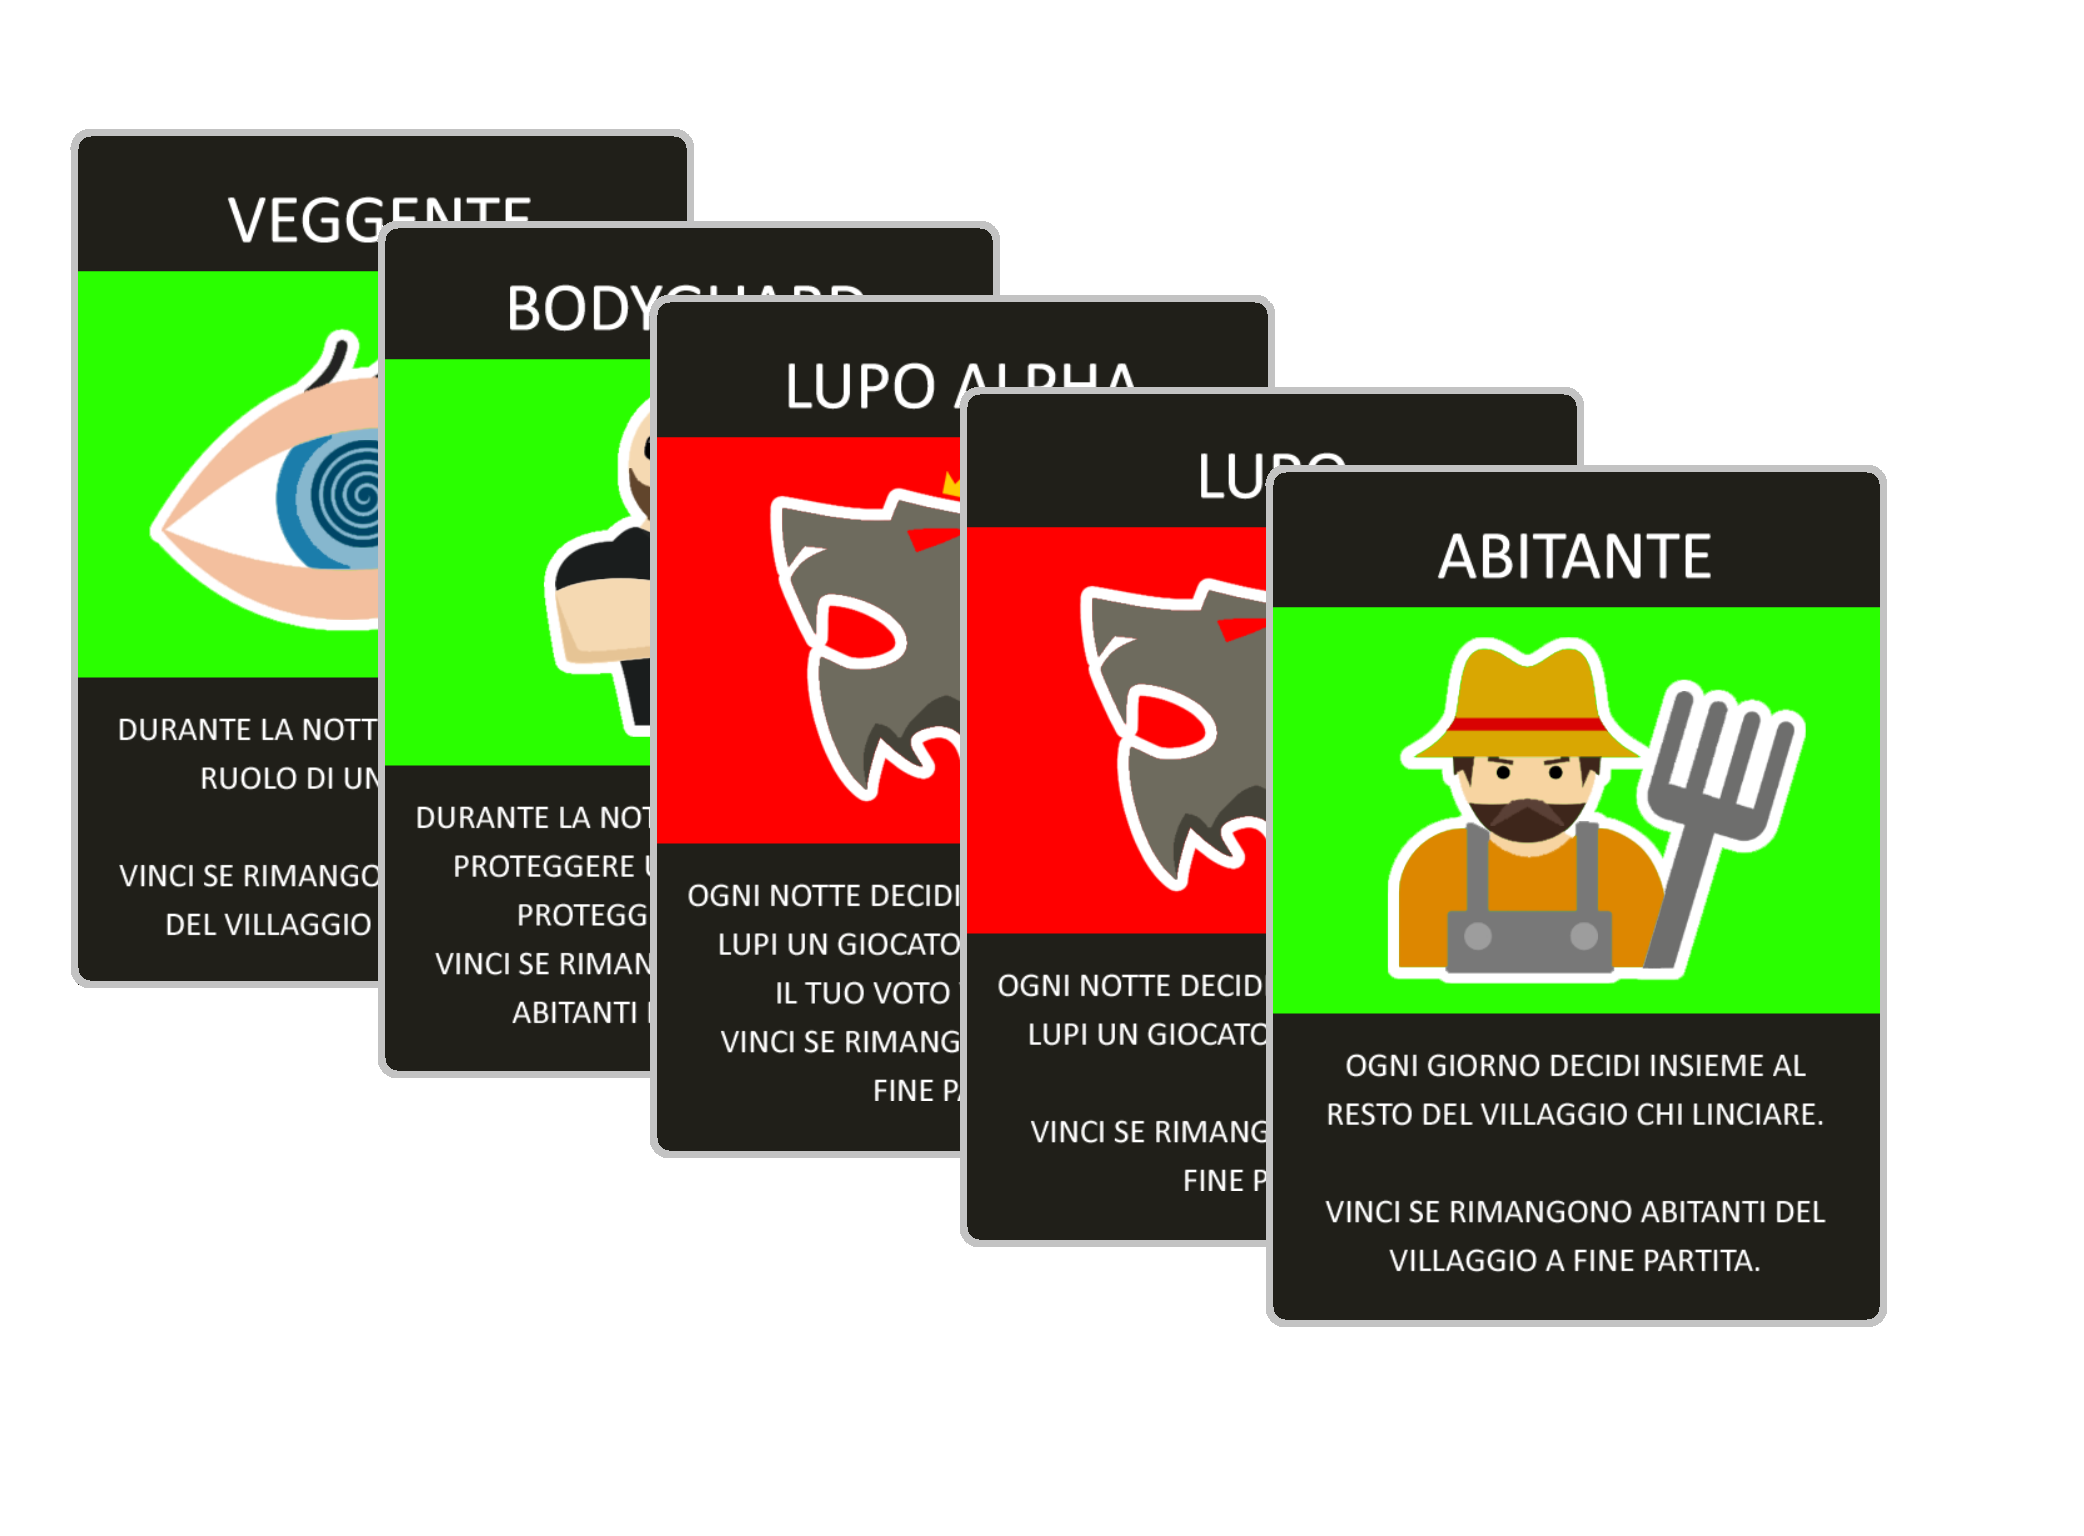
\includegraphics[width=\textwidth]{img/cards.png}
\caption{Ruoli implementati in Lupus}
\label{fig:cards}
\end{figure}
\chapter{Requisiti}
L'obiettivo finale del progetto è quello di creare un applicativo che, basandosi su un'architettura Client-Server ibrida, permetta di ottenere le funzionalità descritte nel capitolo precedente.

\section{Obiettivi}
Il sistema distribuito si baserà su di un'architettura \emph{peer-to-peer}\cite{p2pWikipedia} con discovery server per la gestione della singola partita, durante la quale tutti i client partecipanti, in maniera mista e trasparente tra Web e Mobile, condivideranno le informazioni di gioco mantenendo così uno stato aggiornato e consistente tra loro, permettendo così al sistema di scalare in base alle necessità.

Il server avrà poi un ruolo più centrale per quanto riguarda la persistenza del sistema, grazie alla realizzazione di un database, occupandosi di salvare credenziali ed informazioni relative agli utenti, oltre che informazioni sui risultati di gioco e statistiche aggregate. Infine verranno sfruttati i \emph{container} per permettere all'utente di effettuare il deployment del sistema in maniera automatizzata ed affidabile. 

\section{Artefatti}
Al termine dello sviluppo sono attesi i seguenti deliverables:

\begin{itemize}
    \item Database
    \item Server
    \item Client
\end{itemize}

Le tecnologie che si andranno ad utilizzare per il loro sviluppo sono MongoDB per quanto riguarda il database, Node.js ed in particolare il framework Express per l'implementazione del Server, e per il Client la libreria Javascript React per lo sviluppo della versione Web in combinazione con Bootstrap. Infine verranno utilizzati npm e Docker per quanto riguarda la building automation ed il deployment.


\chapter{Design}
Per lo sviluppo e l'implementazione del sistema è stato scelto lo stack MERN, una variazione dell'originale stack MEAN \cite{meanWikipedia} nella quale Angular viene sostituito da React. Questa architettura permette di creare in maniera semplificata una struttura su tre livelli (\emph{front end, back end, database}) utilizzando solamente JavaScript e JSON.

\begin{figure}[H]
\centering

\includegraphics[width=0.4\textwidth]{img/logos/MERN-logo.png}
\caption{Tecnologie stack MERN}
\label{fig:mern}
\end{figure}

Per quanto riguarda invece le interazioni tra le parti del sistema è stato scelto di utilizzare un'architettura ibrida tra \emph{Client-Server} e \emph{Peer-to-Peer}. Come si può vedere in figura \ref{fig:architettura} il server sarà il punto di snodo tra i client ed il database, svolgendo inoltre la funzione di \emph{discovery server} per quanto riguarda le reti p2p. Ogni client sarà quindi in comunicazione con il server per le funzioni di autenticazione, discovery ed interazioni con il db, ma una volta entrato in un \emph{party} sarà connesso direttamente agli altri client.

\begin{figure}[H]
\centering
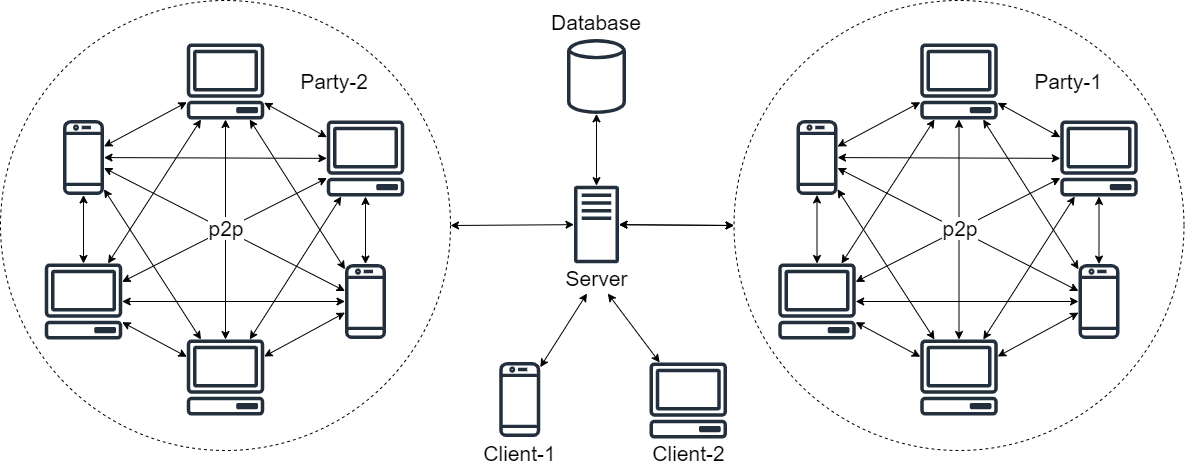
\includegraphics[width=\textwidth]{img/architettura.png}
\caption{Sintesi architettura del sistema}
\label{fig:architettura}
\end{figure}


\section{Struttura del Server} \label{serverStruct}

Il server come detto in precedenza si basa sul framework Express, in accordo con lo stack MERN, e svolge il ruolo di \emph{discovery} per i client che si connettono. Sfruttando la libreria Mongoose all'avvio viene effettuata la connessione al database, dopodiché vengono impostate le route per le richieste HTTP e gli handler per i messaggi ricevuti attraverso le web-socket.\\

Al fine di evitare una crescita incontrollata delle comunicazioni nel caso il sistema venga scalato ad un utilizzo più esteso sono state utilizzate le \emph{rooms} \cite{socketIORooms} messe a disposizione dalla libreria, ovvero dei canali di comunicazione ai quali le socket possono unirsi che permettono al server di inviare messaggi a specifici sottoinsiemi di client senza effettuare broadcast delle informazioni. La singola room corrisponde come concetto a quello di party descritto in precedenza, rappresentando quindi un gruppo di giocatori logicamente isolato dagli altri.

\subsubsection*{Socket}
Per stabilire la connessione tra client e server è stata utilizzata la libreria Socket.io. Per la gestione delle sessioni viene utilizzato un \emph{middleware} \cite{socketIOMiddlewares} che permette di generare identificatori univoci per gli utenti autenticati, dato che l'identificativo del peer viene rigenerato ogni volta, e recuperare quelli presenti in memoria per quelli che ripristinano una connessione.\\
Quando il server riceve una richiesta di connessione da parte di un client viene richiamato il primo handler, \textit{io.on('connection'...)}, che andrà ad associare alla socket tutti gli altri handler, nel codice creati con \textit{socket.on('name', (message)...)}, qui di seguito riportati solo per nome e descrivendo l'eventuale messaggio atteso.

\begin{itemize}
    \item \textbf{disconnect}: Messaggio inviato in automatico dal client al momento della disconnessione, il server modifica lo stato della sessione come non connesso, e lo rimuove dalla room.
    \item \textbf{logout}: Quando un utente effettua il logout l'identificativo associato alla sua sessione viene cancellato completamente.
    \item \textbf{login}: Inviato con un payload contenente username e password, se l'autenticazione va a buon fine viene inviato come risposta e salvato localmente il codice della sessione, diversamente verrà inviato un messaggio di errore.
    \item \textbf{signup}: Anche nel caso della registrazione i campi del payload saranno sempre username e password, la risposta sarà positiva o negativa a seconda dell'esito del salvataggio delle credenziali sul database.
    \item \textbf{room}: Questo messaggio richiede due identificativi, uno per identificare il peer ed uno per la room alla quale ci si vuole unire. Il server a seconda dello stato della room avrà comportamenti leggermente diversi, tutti finalizzati alla comunicazione degli identificativi dei peer ai client della room stessa, facendo sì che tutti possano connettersi tra di loro e formare una effettiva rete p2p.
    \item \textbf{close\_room}: Con l'identificativo della room come payload serve per comunicare al server che nessun altro client potrà più unirsi al canale.
    \item \textbf{peer\_destroyed}: Se il peer viene distrutto completamente verrà anche in questo caso rimosso dalla room e in più l'evento sarà comunicato a tutti i partecipanti alla stessa.
    \item \textbf{save}: Inviato con un payload contenente tutte le informazioni relative alla partita appena conclusa si occuperà di salvarle sul database.
    \item \textbf{send\_stats}: Inviato con uno username come payload risponde inviando tutte le informazioni e statistiche correlate allo storico del giocatore.
    
\end{itemize}


\subsubsection*{Routes}
Per quanto riguarda le richieste HTTP il server utilizza il Router fornito da Express. In una prima fase di sviluppo queste route sono state utilizzate per interagire con il server ed il database, successivamente poi nelle versioni più avanzate del sitema ne sono state mantenute solo alcune ai fini di offrire la possibilità all'utente che esegue il server di visualizzare alcune informazioni utili. Le route in aggiunta a quella di default \emph{"/"} sono divise come segue:

\begin{itemize}
    \item User:
    \begin{itemize}
        \item \textbf{GET - /users}: Ritorna le informazioni relative a tutti gli utenti registrati al server.
        \item \textbf{GET - /user/:username}: Ritorna le informazioni dell'utente identificato dallo username.
        \item \textbf{POST - /user} : Prendendo come parametri username e password crea un nuovo utente nel database.
    \end{itemize}
    \item Game:
    \begin{itemize}
        \item \textbf{GET - /games}: Ritorna le informazioni relative a tutte le partire giocate e salvate sul server.
    \end{itemize}
            
\end{itemize}


\newpage
\section{Struttura del Database}
Il database utilizzato dal sistema è stato strutturato in maniera semplice con l'obiettivo di familiarizzare con le tecnologie impiegate, raggiungendo comunque i requisiti che erano stati prefissati.\\

\begin{figure}[H]
\centering
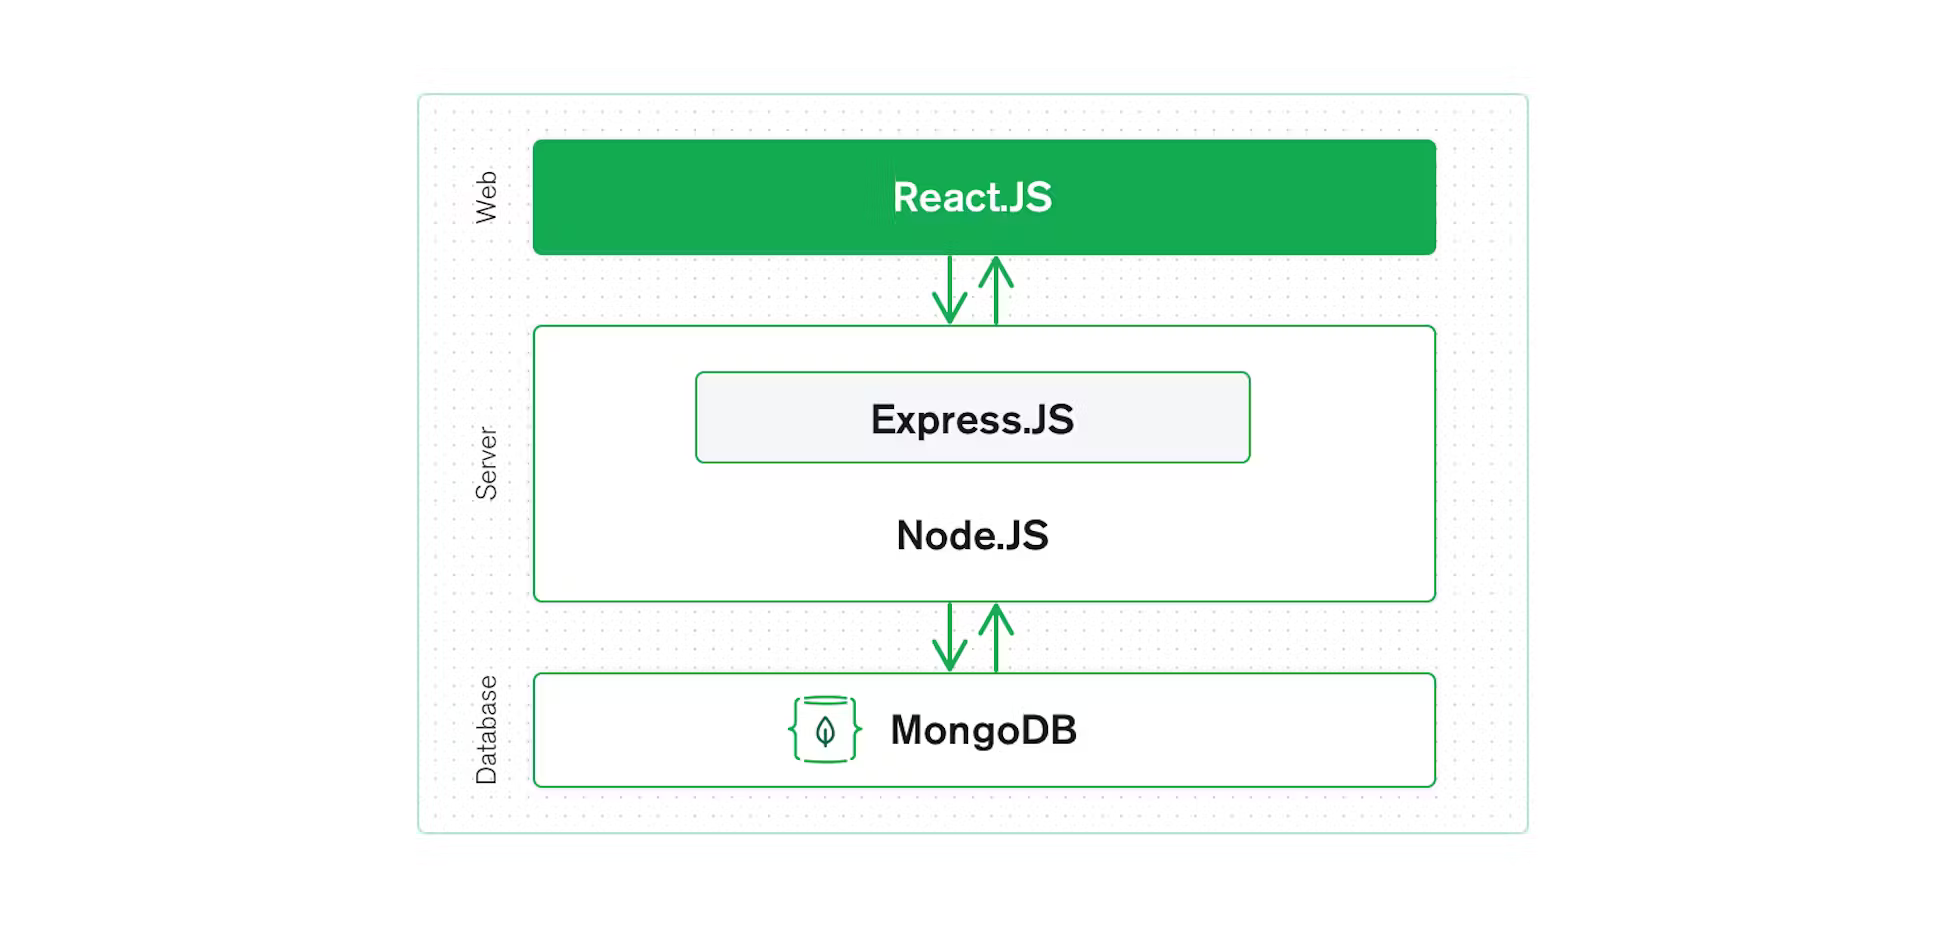
\includegraphics[width=\textwidth]{img/mern-stack.png}
\caption{Stack MERN \cite{mongodbMERN}}
\label{fig:mongodbmern}
\end{figure}


\begin{figure}[H]
\centering
\includegraphics[width=0.8\textwidth]{img/db-classes.png}
\caption{Diagramma delle classi}
\label{fig:dbClasses}
\end{figure}


Come si può vedere nella figura \ref{fig:dbClasses} le informazioni salvate si riassumono in due classi, \emph{user} e \emph{game}. La prima contiene le informazioni relative al singolo utente, ovvero:
\begin{itemize}
    \item \textbf{username:} nome scelto dall'utente in fase di registrazione, univoco all'interno del database.
    \item \textbf{password:} la password impostata che viene salvata come hash utilizzando la libreria \emph{bcript} \cite{bcryptWikipedia}.
    \item \textbf{goodWins/badWins:} statistiche aggregate relative alle vittorie ottenute in base alla squadra di appartenenza.
    \item \textbf{playedGames:} un array contenente gli identificativi delle partite giocate dall'utente.
\end{itemize}
Alcune delle informazioni salvate possono essere considerate ridondanti, come ad esempio il campo \emph{playedGames}, ma sono state pensate per uno stato futuro del sistema nel quale il numero di entità di \emph{game} sarà molto elevato, causando così una possibile complessità computazionale crescente per la ricerca di tutte le partite nelle quali ha partecipato uno specifico giocatore.\\
La classe \emph{game} è composta da:
\begin{itemize}
    \item \textbf{gameCode:} codice univoco utilizzato per identificare la partita.
    \item \textbf{winners:} la squadra vincitrice.
    \item \textbf{players:} un array contenente gli username dei giocatori partecipanti ed il loro relativo ruolo.
    \item \textbf{history:} un array la "storia" della partita, ovvero tutti i sui avvenimenti avvenimenti.
\end{itemize}

\section{Struttura del Client}
Anche il client rispetta lo stack scelto per il sistema e si basa quindi sul framework React. La sua struttura interna si basa su due macro comportamenti coesistenti, comportandosi come client nei confronti del server centralizzato e come peer nei confronti degli altri client connessi.\\

La parte grafica di interfaccia utente è stata realizzata utilizzando i componenti di React.
Sfruttando appunto le caratteristiche di questi ultimi è possibile ridurre il codice prodotto, seguendo il principio d\emph{don't repeat yourself}, riutilizzandoli all'interno di altri componenti, e mantenere una struttura più logica.
Il framework di React nasce come base per lo sviluppo di applicazioni a pagina singola e si occupa solamente del rendering dei dati sul DOM, pertanto la creazione di applicazioni complesse richiede generalmente l'uso di librerie aggiuntive per lo state management e il routing\cite{reactweb}. Per questo progetto sono state rispettivamente le librerie Redux e React Router.

\subsection{Componenti e Router}
L'utilizzo della libreria React Router permette come detto in precedenza di sviluppare un'applicazione strutturata su più pagine, mantenendo così un ordine maggiore all'interno del codice. I componenti comuni a tutta l'applicazione vengono tenuti separati, come ad esempio la \emph{Navbar}, mentre gli altri sono suddivisi sulla base della relativa interfaccia. La struttura delle pagine nel router e delle relative componenti è la seguente:

\begin{itemize}
    \item \textbf{Lupus/ :} partendo dal componente di \emph{Autentication} l'utente verrà reindirizzato verso \emph{Home} nel caso sia già autenticato o verso \emph{Login} in caso opposto.
    \item \textbf{Lupus/lobby :} il router navigherà qui una volta inserito il codice del party mostrando ora il componente \emph{Lobby}.
    \item \textbf{Lupus/game :} avviata la partita verrà invece mostrato il componente \emph{Game}.
    \item \textbf{* :} di default ogni indirizzo non compreso tra i precedenti viene reindirizzato ad una pagina "404" personalizzata.
\end{itemize}

\subsection{Redux}
Per quanto riguarda lo stato del client è stata invece sfruttata la libreria Redux in aggiunta al concetto di stato presente in React. Gli oggetti creati ed utilizzati in questo caso sono i seguenti:
\begin{itemize}
    \item \textbf{game :} contiene tutte le informazioni relative alla singola partita.
        \begin{itemize}
            \item \textbf{gameCode :} codice univoco generato per identificare la partita.
            \item \textbf{partyClosed :} \emph{True} se il party è completo e chiuso.
            \item \textbf{players :} array dei giocatori in partita.
            \item \textbf{phase :} fase della partita.
            \item \textbf{history :} array contenente lo storico della partita.
            \item \textbf{wolfNumber :} numero di lupi impostati.
            \item \textbf{extras :} informazioni su quali personaggi extra sono stati impostati.
        \end{itemize}
    \item \textbf{user :} contiene tutte le informazioni relative all'utente.
        \begin{itemize}
            \item \textbf{username :} nome univoco identificativo.
            \item \textbf{room :} il codice identificativo del party selezionato.
            \item \textbf{token :} identificativo della sessione.
            \item \textbf{stats :} contiene le statistiche ricevute dal server.
        \end{itemize}
    \item \textbf{util :} raccolta di booleani utili al sistema per definirne lo stato.
        \begin{itemize}
            \item \textbf{socketConnected :} stato della socket verso il server.
            \item \textbf{peerConnected :} stato della connessione del peer.
            \item \textbf{isLoading :} stato di caricamento, attesa di informazioni.
            \item \textbf{cardVisible :} necessità di mostrare la carta all'avvio della partita.
        \end{itemize}
\end{itemize}

\newpage
\subsection{Messaggi}
Il client avrà come anticipato due modalità di comunicazione, attraverso websocket con Socket.io potrà inviare messaggi verso il server, mentre sfruttando le API messe a disposizione da PeerJS scambierà le informazioni di gioco con gli altri client.

Per quanto riguarda l'interfaccia del client i messaggi inviati corrispondono a quelli indicati dai \emph{listener} descritti nella sezione \ref{serverStruct}. Segue quindi una panoramica dei messaggi che possono essere ricevuti.


\begin{itemize}
    \item \textbf{connect}: ricevuto al momento della riuscita connessione al server.
    \item \textbf{session}: contiene il codice identificativo della sessione. 
    \item \textbf{signup\_done}: indica l'avvenuta registrazione con successo.
    \item \textbf{room}: ricevuto per conferma dell'inserimento del client in una room.
    \item \textbf{restore\_room}: se la room è stata chiusa in precedenza ed il client ne esce questo messaggio viene ricevuto in fase di rientro.
    \item \textbf{user\_stats}: messaggio contenente le informazioni sulle statistiche del giocatore.
    \item \textbf{new\_peer}: messaggio utilizzato dal server per notificare l'entrata di un nuovo peer al quale il client dovrà connettersi.
    \item \textbf{restore\_peer}: se era già stata effettuata in precedenza la connessione allo stesso client allora il server invierà un messaggio specifico.
    \item \textbf{peer\_removed}: se un client si disconnette il server notifica la necessità di rimuovere il peer.
    \item \textbf{room\_closed}: il server usa il messaggio per comunicare che la room è chiusa e non verranno più accettati altri utenti.
    \item \textbf{room\_unavailable}: quando un utente prova ad entrare in una room già chiusa riceverà questo messaggio in risposta.
    \item \textbf{*\_error}: i messaggi di tipo \_error possibili sono relativi a \emph{connect}, \emph{login} e \emph{signup}, ognuno può trasportare le informazioni di un errore specifico.
    
\end{itemize}


\newpage

\section{Interfaccia Utente}
Lo sviluppo dell'interfaccia utente è stato effettuato in maniera incrementale consultando amici e colleghi del corso per meglio definire le componenti fondamentali e gli scenari di utilizzo. Dopo una prima fase di bozzetti su carta sono stati disegnati i wireframe del progetto utilizzando Figma. La parte di definizione ed implementazione ha poi tenuto conto dei criteri di accessibilità di cui si parlerà in seguito.

\subsection{Wireframe}
Le interfacce sono state sviluppate seguendo il criterio \emph{mobile-first}, qui di seguito verranno riportati esempi di visualizzazione sia mobile che da desktop. Tutte le schermate avranno una \emph{navbar} contenente il logo dell'applicazione e un menu a tendina che potrà contenere diverse funzionalità a seconda dello stato del sistema.\\

La prima schermata che si presenterà all'utente sarà quella di accesso, visibile nelle figure \ref{fig:androidLogin} e \ref{fig:pcLogin}, dalla quale sarà possibile registrarsi inserendo delle nuove credenziali o accedere attraverso quelle inserite in precedenza.



\begin{figure}[H]
\centering
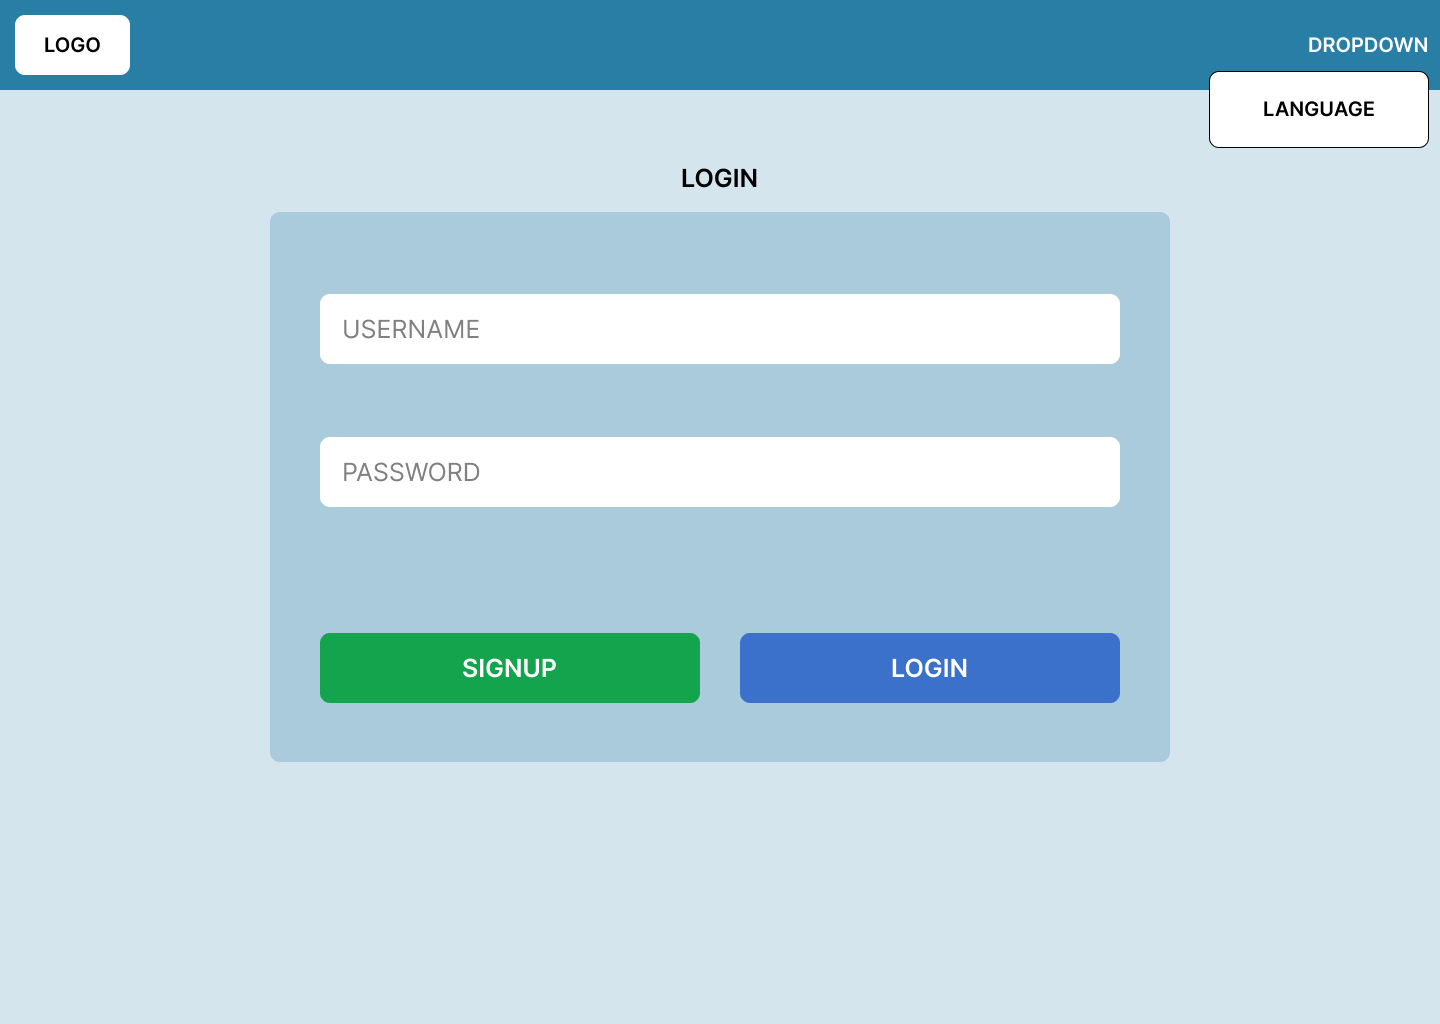
\includegraphics[width=\textwidth]{img/figma/Wireframe-1.png}
\caption{Schermata di login}
\label{fig:pcLogin}
\end{figure}


A seguire una volta effettuato il login l'utente potrà inserire un codice identificativo di una room da creare o alla quale unirsi, attraverso un form visibile nella figura \ref{fig:pcRoom}. Nella stessa figura è mostrata come esempio anche una notifica che il sistema potrà mandare all'utente sfruttando la libreria \emph{react-notifications}\cite{npmjsReactnotifications}.

\begin{figure}[H]
\centering
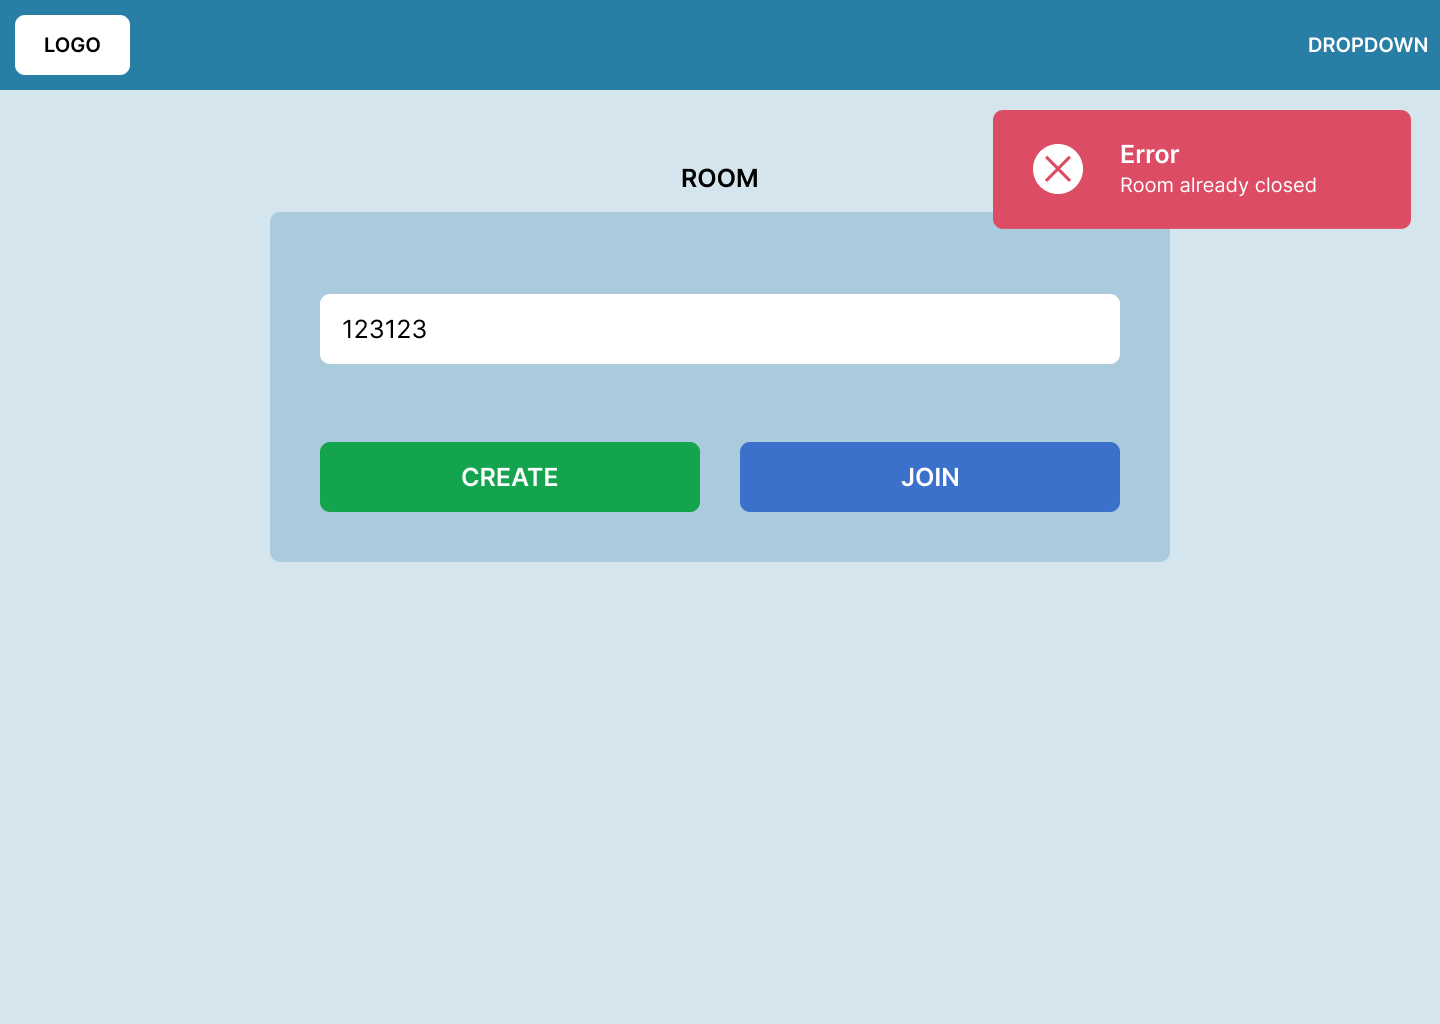
\includegraphics[width=\textwidth]{img/figma/Wireframe-2.png}
\caption{Schermata di selezione della room}
\label{fig:pcRoom}
\end{figure}

\newpage

Una volta all'interno all'utente verrà mostrata una schermata come quella in figura \ref{fig:pcLobby} nella quale si avrà la possibilità di chiudere la room una volta raggiunto il numero minimo di giocatori richiesto. Successivamente in base alle specifiche di implementazione del gioco sarà data la possibilità attraverso un modale di modificare le impostazioni di gioco, come il numero di lupi od eventuali personaggi extra che si vogliono utilizzare.

\begin{figure}[H]
\centering
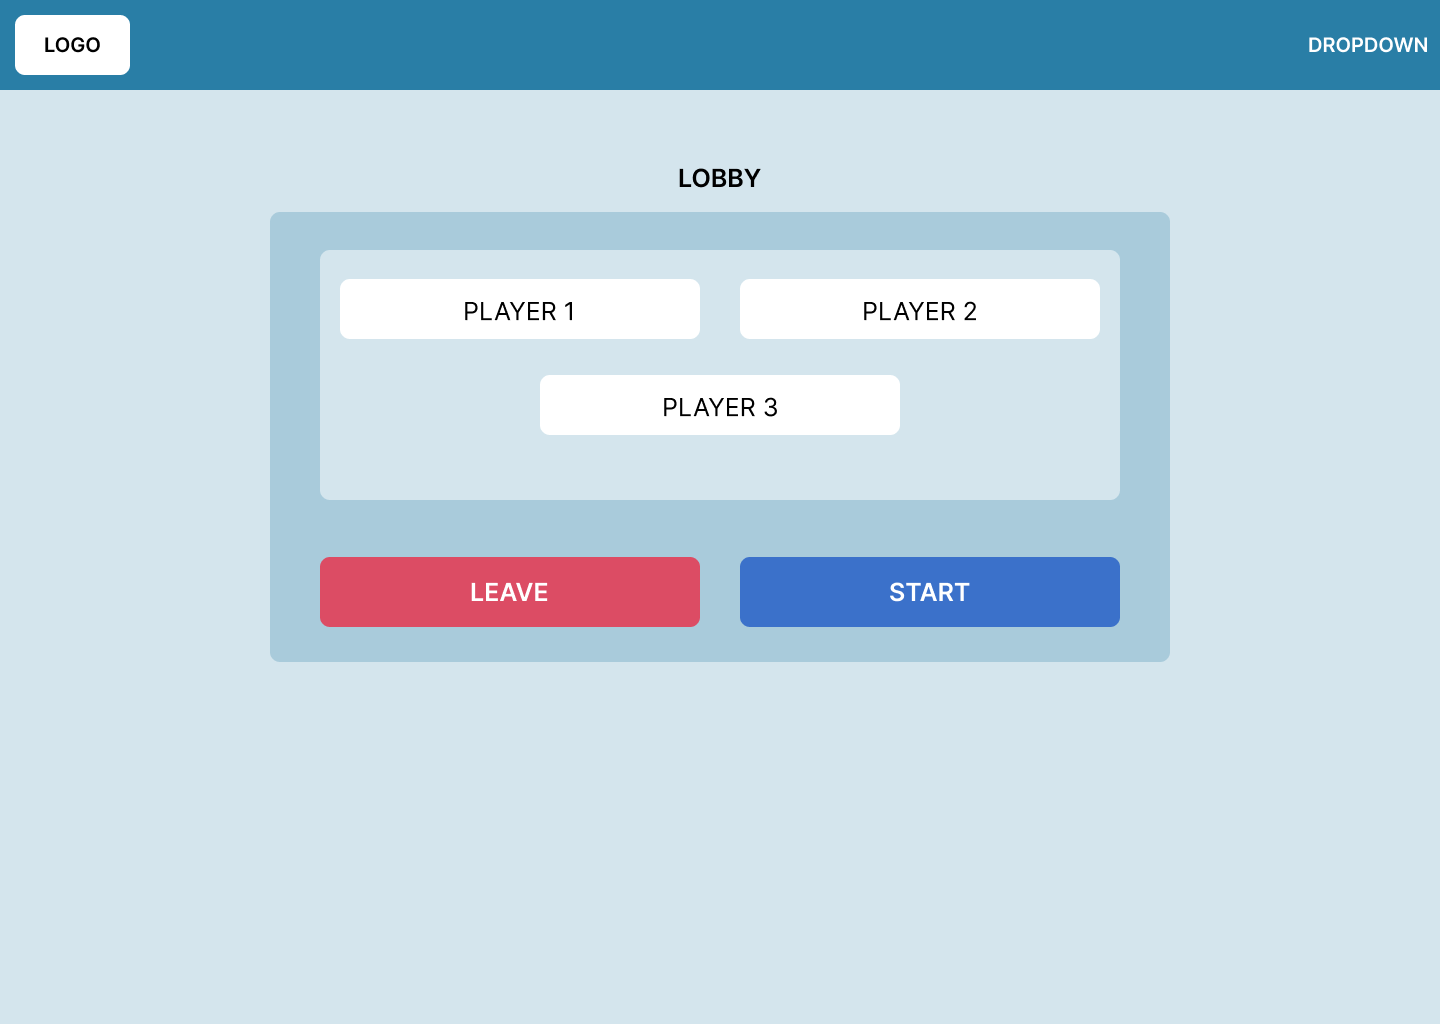
\includegraphics[width=0.9\textwidth]{img/figma/Wireframe-3.png}
\caption{Schermata interna alla room}
\label{fig:pcLobby}
\end{figure}

\newpage

Dopo aver avviato la partita la schermata di gioco sarà quella mostrata nella figura \ref{fig:pcGame}, strutturata su tre colonne contenenti le informazioni necessarie, l'elenco dei giocatori partecipanti, la carta rappresentante il ruolo del giocatore e lo storico degli avvenimenti della partita. In base alla fase di gioco nella parte alta della schermata verrà poi mostrato un ulteriore elenco dei giocatori tra i quali scegliere chi si vuole votare. Nella visualizzazione mobile mostrata nella figura \ref{fig:androidGame} le colonne verranno disposte verticalmente in maniera reattiva in base alla dimensione della finestra.

\begin{figure}[H]
\centering
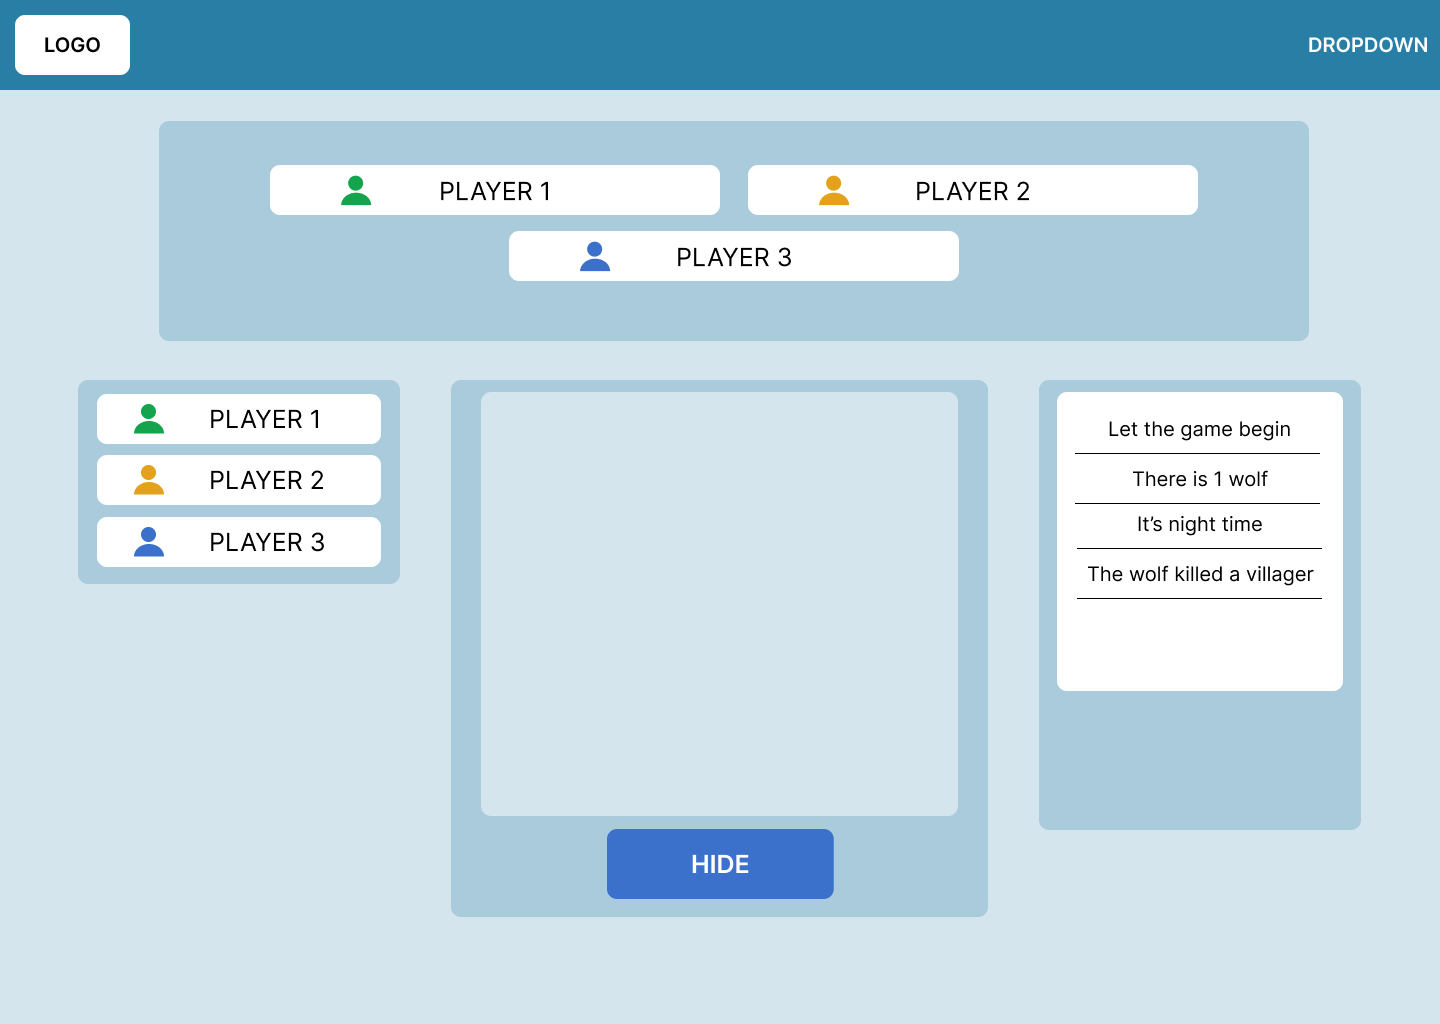
\includegraphics[width=0.9\textwidth]{img/figma/Wireframe-4.png}
\caption{Schermata di gioco}
\label{fig:pcGame}
\end{figure}


\begin{figure}[H]
    \centering
    \begin{minipage}{0.45\textwidth}
        \centering
        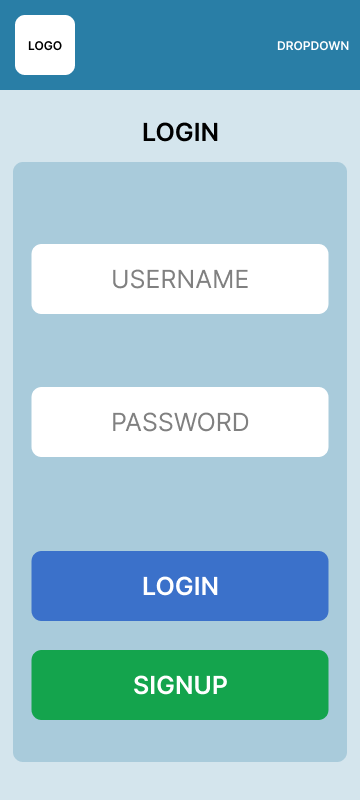
\includegraphics[width=0.9\textwidth]{img/figma/AndroidLarge-1.png} \caption{Schermata di login per dispositivo mobile}
        \label{fig:androidLogin}
    \end{minipage}\hfill
    \begin{minipage}{0.45\textwidth}
        \centering
        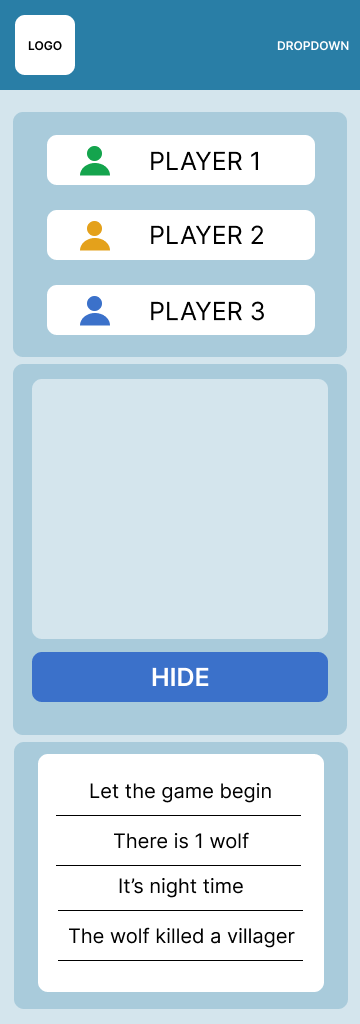
\includegraphics[width=0.9\textwidth]{img/figma/AndroidLarge-2.png} \caption{Schermata di gioco per dispositivo mobile}
        \label{fig:androidGame}
    \end{minipage}
\end{figure}

\newpage

\subsection{Accessibilità}
Durante lo svolgimento di questo progetto i criteri di accessibilità sono stati tenuti in considerazione per ottenere un prodotto finale che li rispettasse al meglio. 
Oltre ai requisiti utili per l'utilizzo di screen reader, come i tag degli elementi ed i testi alternativi alle immagini, è stata posta una particolare attenzione ai contrasti e all'utilizzo dei colori.\\
Alcune di queste scelte sono state prese basandomi sulla mia diretta esperienza in quanto daltonico. La forma di daltonismo più comunemente riscontrata è la deuteranopia (o deuteranomalia), la quale inficia la capacità di distinguere i colori sull'asse rosso-verde. Per questo motivo la palette scelta per le interfacce è stata scelta a partire dal colore identificato da \emph{\#297ea6}, contenente una bassa percentuale di tinta rossa.\\
Per rendere poi accessibile l'applicazione anche a possibili utenti non italiani, come ad esempio studenti in erasmus, in accordo con il concetto di \emph{internationalization} \cite{internationalizationWikipedia} è stata utilizzata la libreria \emph{i18next} \cite{i18next} di react per inserire anche la lingua inglese come alternativa. La schermata di selezione nella sua versione mobile è riportata nella figura \ref{fig:language_mobile}.

\subsection{Interfacce finali}
Le interfacce finali sono riportate al termine della relazione attraverso screenshots della versione desktop e mobile, rispettivamente contenuti nelle appendici \ref{appendix:desktop} e \ref{appendix:mobile}, raccolti durante una demo di gioco.\\


\chapter{Tecnologie}
La maggior parte delle tecnologie impiegate per lo sviluppo di questo progetto sono state definite nelle prime fasi di design, oltre che in fase di proposta dello stesso. Alcune librerie o specifici framework invece sono stati il risultato di scelte nate durante la fase di implementazione. Qui di seguito verranno descritte alcune tra le principali tecnologie utilizzate suddividendole tra quelle trasversali a tutto il progetto e quelle specifiche delle componenti di server, database e client.

\section{Tecnologie trasversali}

\subsection{NPM}
Node.js \cite{nodejsWikipedia} è un \emph{runtime system} multipiattaforma per l'esecuzione di codice JavaScript, costruito sul motore JavaScript V8 di Google Chrome.
Node.js dispone di una grande quantità di moduli scritti completamente in Javascript.
Essendo il progetto open-source è inoltre possibile per gli sviluppatori aggiungere i propri moduli in modo da renderli disponibili pubblicamente.

Il gestore di pacchetti predefinito per l'ambiente si chiama Node Package Manager.\emph{npm} può essere richiamato tramite linea di comando usando la seguente sintassi:
\begin{verbatim}
    npm <command> [args]
\end{verbatim}
Il comando base per ottenere un pacchetto è:
\begin{verbatim}
    npm install packet_name
\end{verbatim}
Tutte le dipendenze ed i conflitti vengono gestiti automaticamente \cite{npmDoc}. Grazie a Node è anche possibile per esempio creare un progetto React utilizzando il comando seguente:
\begin{verbatim}
    npx create-react-app project
\end{verbatim}
\emph{npx} è uno strumento integrato in npm in grado di eseguire pacchetti, anche se non sono ancora installati nel sistema.
Sarà poi possibile avviare il server di sviluppo utilizzando i seguenti comandi:
\begin{verbatim}
    cd project
    npm start
\end{verbatim}
L'interfaccia sarà poi visualizzabile all'indirizzo \emph{http://localhost:3000}.

\begin{figure}[H]
\centering

\includegraphics[width=0.3\textwidth]{img/logos/npm_logo.png}
\caption{npm logo}
\label{fig:npm}
\end{figure}

\subsection{Socket.io}
Socket.io è una libreria JavaScript che fornisce un servizio molto simile alle originali Web-Socket. Socket.io offre delle API JavaScript cross-browser che permettono la creazione di un canale di comunicazione full-duplex tra domini a bassa latenza tra il browser e il server web.

Socket.io tenta di utilizzare prima di tutto le WebSocket native. In caso fallisca (in caso di incompatibilità coi sistemi o a causa di altri problemi)
ricorrerà all'utilizzo di polling HTTP.

Socket.io è stato progettato per funzionare con tutti i browser moderni (97\% di compatibilità nel 2020) e in ambienti che non
supportano il protocollo WebSocket, ad esempio dietro proxy aziendali restrittivi.\\

Oltre alle funzionalità offerte da una tradizionale WebSocket, Socket.io offre inoltre le seguenti features:
\begin{itemize}
    \item reliability (switch a polling HTTP nel caso la connessione WebSocket non possa essere stabilita)
    \item riconnessione automatica
    \item buffering dei pacchetti
    \item acknowledgments
    \item broadcast a tutti i client o ad un sottoinsieme di essi (Room)
    \item multiplexing
\end{itemize}

\begin{figure}[H]
\centering

\includegraphics[width=0.4\textwidth]{img/logos/socketIO_logo.jpg}
\caption{Socket.io logo}
\label{fig:socketio}
\end{figure}

\subsection{Docker}
Docker è un sistema open-source tramite il quale è possibile automatizzare il processo di deployment di applicazioni all'interno di contenitori software.
Docker implementa API di alto livello per gestire \emph{container} che eseguono processi in ambienti isolati.

Utilizzando i container dunque le risorse possono essere isolate, i servizi limitati e i processi avviati in modo da avere una prospettiva completamente privata del sistema operativo, col loro proprio identificativo, file system e interfaccia di rete. Più container condividono lo stesso kernel, ma ciascuno di essi può essere costretto ad utilizzare una certa quantità di risorse, come la CPU, la memoria e l'I/O.

L'utilizzo di Docker per creare e gestire i container può semplificare la creazione di sistemi distribuiti, permettendo a diverse applicazioni o processi di lavorare in modo autonomo sulla stessa macchina fisica o su diverse macchine virtuali. Ciò consente di effettuare il deployment di nuovi nodi solo quando necessario.

Al fine di creare un container Docker sarà necessario specificare un \emph{Dockerfile} per ogni servizio erogato. 
Similmente ai gitignore per il versioning git, è possibile definire dei \emph{dockerignore} per segnalare a docker quali file ignorare durante la copia dei file all'interno del container. Per gestire invece applicazioni composte da più servizi sarà possibile utilizzare \emph{Docker Compose}, uno strumento che permette con un solo comando di avviare un intero sistema isolato gestendo nello specifico dipendenze tra servizi, volumi e reti.

\begin{figure}[H]
\centering

\includegraphics[width=0.5\textwidth]{img/logos/docker_logo.png}
\caption{Docker logo}
\label{fig:docker}
\end{figure}

\section{Tecnologie Server}
\subsection{Node.js}
Node.js \cite{nodejsWikipedia} è un \emph{runtime system} multipiattaforma per l'esecuzione di codice JavaScript, costruito sul motore JavaScript V8 di Google Chrome, progettato per creare applicazioni di rete scalabili. Grazie al suo funzionamento molte connessioni possono essere gestite contemporaneamente, per ognuna delle quali verrà invocata una callback, rendendo Node attivo solo al momento necessario.\\

Node.js implementa un'architettura event-driven, facendo dunque affidamento su un event loop. Non esiste alcuna chiamata per avviare il ciclo: Node.js entra semplicemente nel ciclo degli eventi dopo aver eseguito lo script di input e, analogamente, esce dal ciclo di eventi quando non ci sono più callback da eseguire. Questo comportamento è simile a JavaScript in browser: il ciclo degli eventi è nascosto all'utente.
Per natura dell'event loop, Node è single-threaded, ma è possibile, su necessità, effettuare delle fork per sfruttare al meglio i core offerti dalla macchina creando nuovi thread.

\begin{figure}[H]
\centering

\includegraphics[width=0.3\textwidth]{img/logos/nodejs_logo.png}
\caption{Node.js logo}
\label{fig:nodejs}
\end{figure}

\subsection{Express}
Express è un framework web per Node.js che semplifica lo sviluppo di applicazioni web e API. Fornisce una serie di funzionalità per gestire richieste HTTP, definire \emph{rotte}, elaborare dati di input e gestire le risposte. Express è estremamente flessibile e leggero, consentendo agli sviluppatori di creare rapidamente applicazioni web scalabili e con ottime prestazioni.

Una delle caratteristiche principali di Express è il concetto di \emph{middleware}, ovvero funzioni che possono essere eseguite prima, durante o dopo il processo di gestione delle richieste. Questo consente agli sviluppatori di rendere modulare il codice e aggiungere facilmente funzionalità come autenticazione e gestione degli errori.

Express segue il paradigma di programmazione event-driven di Node.js e si integra perfettamente con esso. Può essere utilizzato insieme ad altri moduli Node.js per gestire aspetti specifici delle applicazioni web, come la gestione delle sessioni utente o la connessione al database.

Grazie alla sua vasta adozione nella comunità Node.js, Express ha una vasta gamma di plugin e middleware disponibili, che permettono agli sviluppatori di estendere facilmente le funzionalità base del framework per adattarsi alle esigenze specifiche del progetto.

In sintesi, Express è un potente framework per lo sviluppo di applicazioni web con Node.js, che offre una combinazione di flessibilità, prestazioni e facilità d'uso.

\begin{figure}[H]
\centering

\includegraphics[width=0.4\textwidth]{img/logos/expressjs_logo.png}
\caption{Express logo}
\label{fig:express}
\end{figure}

\subsection{Mongoose}
Mongoose è una libreria per Node.js che permette di creare degli \emph{Schema} per rappresentare i dati da archiviare nel sistema.
Ogni Schema è associato ad una collezione nel Database di MongoDB.
Mongoose viene utilizzato per la creazione del proprio model, essendo possibile creare delle istanze dallo Schema attraverso delle \emph{Factory} ed utilizzarli come dei semplici oggetti Javascript.
Oltre ad offrire metodi aggiuntivi già pronti per salvare i dati all'interno del database è possibile creare funzioni che solo oggetti appartenenti ad un relativo schema possono richiamare, rendendo la modellazione simile all'object-oriented.\\

\begin{figure}[H]
\centering

\includegraphics[width=0.3\textwidth]{img/logos/mongoose_logo.png}
\caption{Mongoose logo}
\label{fig:mongoose}
\end{figure}

\section{Tecnologie Database}
\subsection{MongoDB}
MongoDB è un DBMS NoSQL, cioè non utilizza un meccanismo di persistenza relazionale come un tradizionale SQL.
Il modello NoSQL non è unico e può dunque utilizzare varie strutture dati per sostituire le tabelle con campi uniformi utilizzate in SQL.

In particolare MongoDB utilizza un modello orientato al documento, dove le informazioni sono memorizzate in una struttura gerarchica ad albero ed un qualsiasi numero di campi con qualsiasi lunghezza può essere aggiunto. I campi a loro volta possono contenere aggregati di dati composti da più elementi o da strutture annidate.

I DBMS orientati al documento offrono alcuni vantaggi, specialmente in ambito web, rispetto ai tradizionali RDBMS. Si ottengono maggior flessibilità dei dati, utile per avere meno rigidità in fase di sviluppo o, in generale, per scenari in cui i dati memorizzati non sono sempre uniformi, e una maggior facilità nella trasposizione in strutture dati nel codice in quanto i JSON, utilizzati da MongoDB, trovano una corrispondenza uno ad uno con esse. Il trade-off nell'avere una struttura meno rigida è però il rischio di duplicazione di dati ed inconsistenze, per cui è richiesta al progettista una maggiore cautela nella manipolazione di dati.

\begin{figure}[H]
\centering

\includegraphics[width=0.3\textwidth]{img/logos/mongo_logo.png}
\caption{MongoDB logo}
\label{fig:mongodb}
\end{figure}


\section{Tecnologie Client}

\subsection{React.js}
React è un framework open-source che permette di implementare applicazioni web seguendo i principi della programmazione ad oggetti. In modo particolare risulta essenziale descrivere tre concetti chiave:
\begin{itemize}
    \item \textbf{JSX:} è un'estensione della sintassi di JavaScript.\cite{introduzione_jsx_react} Permette di unire gli aspetti di html come linguaggio di template agli aspetti di JavaScript come linguaggio di scripting in una forma che ne aumenta semplicità e leggibilità. Gli elementi JSX vengono utilizzati nelle definizioni delle funzioni di rendering semplificando la costruzione della UI. Attraverso JSX si può richiamare un componente React tramite con un meccanismo analogo ai tag in html.
    \item \textbf{Componenti:} attraverso un componente\cite{componente_react} si va a definire quella che risulta essere a tutti gli effetti una classe. Il componente, definito da uno o più costruttori, contiene uno stato, il quale verrà mantenuto, ed eventualmente aggiornato, durante tutto il ciclo di vita dello stesso. È possibile ricevere dati ed istruzioni da altri componenti attraverso le props.
    \item \textbf{Stato:} è un insieme di proprietà di un componente.\cite{state_e_lifecycle_react} Queste proprietà possono variare a seguito dell'interazione con altri componenti o come azione del componente stesso nel caso esso esegua delle azioni a cadenza temporale. In React lo stato risulta inoltre fondamentale ai fini di ottenere un aggiornamento delle interfacce performante. Ogni componente React deve obbligatoriamente definire una funzione \emph{render()}. Attraverso di essa verrà ritornato il contenuto da renderizzare. React cambierà il contenuto della UI, utilizzando quindi risorse, solamente quando vi saranno delle modifiche nel contenuto ritornato dalla funzione \emph{render()}. Utilizzando dunque le proprietà che definiscono lo stato del componente all'interno di questa funzione sarà possibile ridurre al minimo il numero di volte in cui l'applicazione verrà renderizzata, riflettendo i cambiamenti di stato del componente.    
\end{itemize}

React infine introduce anche i componenti funzione, che di fatto svolgono la stessa funzione dei componenti precedentemente descritti, ma con una sintassi più concisa.

\begin{figure}[H]
\centering

\includegraphics[width=0.2\textwidth]{img/logos/react_logo.png}
\caption{React logo}
\label{fig:react}
\end{figure}


\subsection{Redux}

Redux \cite{caratteristiche_redux} è un \emph{contenitore di stato} per applicazioni JavaScript. Gode di quattro caratteristiche fondamentali per progetti portata medio-grande:
\begin{itemize}
  \item \textbf{Deterministico:} aspetto fondamentale nelle applicazioni web di ogni genere è il determinismo. L'oneroso compito di far collaborare tutti i componenti al fine di ottenere un comportamento predicibile viene largamente semplificato dall'utilizzo di questo framework.
  \item \textbf{Centralizzato:} avere stato e logica centralizzati permette di ottenere rapidamente delle feature di fondamentale importanza, come funzioni di "annulla" e "ripeti" che permettono di muoversi agilmente tra lo storico degli stati. Un approccio centralizzato garantisce inoltre una consistenza maggiore dei dati, rendendo possibile modificarli solamente attraverso specifiche funzioni, le azioni, create durante la definizione della struttura dati.
  \item \textbf{Debug oriented:} attraverso semplici plugin browser come Redux DevTools risulta immediato il debug dell'applicazione. Attraverso questi tool si ottiene una visione completa dello stato dei dati e della sua evoluzione nel tempo, riuscendo ad identificare con precisione quando e soprattutto perché lo stato abbia subito delle modifiche.
  \item \textbf{Flessibile:} Redux funziona con ogni layer di UI e, essendo ormai uno strumento consolidato, dispone di un solido supporto e una vasta proposta di plugin e pacchetti aggiuntivi per ogni esigenza.
\end{itemize}
Per comprendere come queste caratteristiche si concretizzino risulta fondamentale comprendere tre concetti chiave nella struttura di Redux:
\begin{itemize}
  \item \textbf{Store:} è un oggetto che contiene l'intera struttura ad albero dello stato.\cite{store_redux} Fornisce metodi per la lettura dello stato corrente.
  \item \textbf{Reducer:} definiscono la struttura dello store.\cite{reducer_redux} Vi possono essere più reducer all'interno di una stessa applicazione, al fine di meglio suddividere lo stato.
  \item \textbf{Azioni:} permettono di modificare il contenuto dello store.\cite{azioni_redux} Essendo queste l'unico modo per alterare lo stato attuale, qualsiasi componente che voglia agire sullo stato deve passare per le azioni definite.
\end{itemize}
Ci sono alcune motivazioni che portano alla scelta di utilizzare questo strumento in aggiunta allo stato messo a disposizione da React. Quest'ultimo pur essendo uno strumento molto potente, pone davanti a delle limitazioni.

Non è raro che più componenti all'interno dell'applicazione debbano fare riferimento allo stesso dato, per cui la presenza di uno stato comune evita di dover implementare meccanismi ad hoc di sincronia tra gli stati dei due componenti. Lo stato di ogni componente, attraverso strumenti preesistenti, sarà dunque sincronizzato con la struttura principale.

React inoltre, data la sua natura orientata alla programmazione reattiva, incoraggia la propagazione dell'informazione solo in una direzione: da un componente padre verso un componente figlio. La presenza delle azioni Redux risolve questo problema in quanto ogni cambiamento apportato allo stato Redux si rifletterà su tutti i componenti React che utilizzano quel particolare dato, in maniera trasparente nei confronti della loro gerarchia.

\begin{figure}[H]
\centering
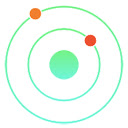
\includegraphics[width=0.3\textwidth]{img/logos/redux_devtool.jpg}
\caption{Redux logo}
\label{fig:redux}
\end{figure}

\subsection{Bootstrap}

Bootstrap è stato creato nel 2010, tramite Twitter, da @mdo and @fat. È rapidamente diventato il framework più popolare per il front-end a livello mondiale. Con le prime release della versione 2 vennero introdotti i primi fogli di stile per aggiungere funzionalità riguardanti il design responsive. Con l'uscita della versione 3 l'intera libreria è stata ripensata e riscritta per offrire supporto al design responsive con un approccio mobile-first. La versione 4 di Bootstrap, ovvero quella attuale, ha subito infine due principali cambiamenti nella sua architettura:
\begin{itemize}
    \item una migrazione a Sass, un'estensione del linguaggio CSS che permette l'uso di variabili e di funzioni,
    \item l'uso di CSS flexbox, ovvero contenitori per elementi.
\end{itemize}

Come detto in precedenza, Bootstrap adotta un approcio mobile-first. L'assunzione di base è che la maggior parte dei visitatori utilizzeranno uno smartphone a causa del sempre più crescente utilizzo di questo tipo di dispositivi. L'utilizzo continuo di media query è alla base di ogni layout creato utilizzando Bootstrap \cite{bootstrap}. Moltissime classi offerte utilizzano i cosiddetti breakpoints. Si tratta di meccanismi che permettono di nascondere, mostrare o modificare il comportamento degli elementi a cui vengono applicate in base alla risoluzione dello schermo del visitatore.
Bootstrap mette a disposizione i seguenti breakpoints:
\begin{minted}{css}
// Small devices (landscape phones, 576px and up) KEYWORD:sm
    @media (min-width: 576px) { ... }
    
// Medium devices (tablets, 768px and up) KEYWORD:md
    @media (min-width: 768px) { ... }
    
// Large devices (desktops, 992px and up) KEYWORD:lg
    @media (min-width: 992px) { ... }
    
// Extra large devices (large desktops, 1200px and up) KEYWORD:xl
    @media (min-width: 1200px) { ... } 
\end{minted}
Segue un rapido esempio per l'uso dei breakpoints. Per la gestione dei margini e del padding Bootstrap mette a disposizione le classi di tipo 
\begin{verbatim}
    {property}{sides}-{breakpoint}-{size}
\end{verbatim}
\begin{itemize}
    \item \textbf{property:} assume valore\textbf{m} se si vuole aggiungere un margine, \textbf{p} se si vuole aggiungere del padding.
    \item \textbf{sides:} assume valore\textbf{t} per top, \textbf{b} per bottom, \textbf{r} per right, \textbf{l} per left, \textbf{x} per right e left, \textbf{y} per top e bottom.
    \item \textbf{breakpoints:} se omesso, la classe funziona su qualsiasi tipo di schermo, anche i più piccoli, altrimenti funziona solo sugli schermi più grandi anche solo di un pixel del breakpoint specificato.
    \item \textbf{size:} Bootstrap non utilizza valori statici per specificare di quanto deve essere il padding o il margine. Il valore che può assumere size va da 0 a 5, e sono valori che indicano quando deve essere grande il moltiplicatore che gestisce lo spazio. \textbf{0} significa nessun padding o margine.
\end{itemize}
Seguendo queste indicazioni se si desidera applicare un piccolo margine a destra ad un determinato elemento solo se visualizzato su uno schermo con larghezza maggiore di 992px, le classi che l'elemento dovrà assumere saranno \emph{mr-0 mr-lg-2}. Appartenere alla prima classe, \emph{mr-0}, significa nessun margine a destra su qualsiasi tipo di schermo, mentre per la seconda, \emph{mr-lg-2}, vuol dire invece avere un margine a destra con proporzione 2 solo su schermi più grandi di 992px. Combinando insieme le due classi otteniamo un margine che varia in maniera reattiva alla dimensione dello schermo\cite{bootstrapDoc}.

\begin{figure}[H]
\centering

\includegraphics[width=0.3\textwidth]{img/logos/bootstrap_logo.png}
\caption{Bootstrap logo}
\label{fig:bootstrap}
\end{figure}


\subsection{PeerJS}

PeerJS è una libreria JavaScript open-source nata per semplificare la creazione di applicazioni \emph{peer-to-peer} in modo trasparente e affidabile. Utilizzando WebRTC, ovvero Web Real-Time Communication, PeerJS permette di stabilire connessioni dirette tra i browser senza la necessità di server intermediari. Questo approccio decentralizzato riduce la latenza e il carico di lavoro sul server, migliorando l'efficienza e la scalabilità delle applicazioni P2P.

Sfruttando PeerJS è possibile creare e gestire connessioni P2P in modo semplice, avendo a disposizione API intuitive per aprire, accettare e gestire le connessioni. La libreria gestisce automaticamente aspetti complessi come il \emph{signaling} e il trasporto dei dati attraverso i peer connessi, consentendo di concentrarsi maggiormente sulla logica dell'applicazione anziché sulle complessità della comunicazione in tempo reale.

Tra le funzionalità offerte utili per la creazione di questo tipo di applicazioni le principali sono la trasmissione di dati in tempo reale, la condivisione di file e la comunicazione audio/video. Inoltre, essendo basato su WebRTC, PeerJS è compatibile con la maggior parte dei browser moderni e fornisce quindi una soluzione sicura e di facile utilizzo.

Per poter connettere i peer l'un l'altro è necessario però avere un server che svolga il compito di \emph{connection broker}, per cui non riceverà nessun dato della rete P2P. Per quanto riguarda l'hosting del server, PeerJS offre due opzioni:
\begin{itemize}
    \item utilizzare il PeerServer Cloud fornito direttamente dagli sviluppatori della libreria, che è una versione cloud-hosted gratuita del PeerServer ufficiale. Questa opzione è conveniente per chi non ha specifiche necessità e preferisce una soluzione facile da implementare,
    \item eseguire il proprio PeerServer, utilizzando il codice sorgente open-source scritto in Node.js disponibile online. Questa opzione offre maggiore controllo e flessibilità, ma richiede competenze tecniche per l'installazione e la configurazione.
\end{itemize}

\begin{figure}[H]
\centering

\includegraphics[width=0.4\textwidth]{img/logos/peerjs_logo.png}
\caption{PeerJS logo}
\label{fig:peerjs}
\end{figure}
\chapter{Codice}
Nel seguente capitolo verranno riportati alcuni estratti del codice implementato per il progetto, con l'obiettivo di evidenziare aspetti affrontati durante lo sviluppo che sono stati ritenuti interessanti.

\section{Server}

\subsection{Routes}

Nell'estratto seguente è possibile vedere come siano definite le rotte all'interno del server. Si dividono in tre gruppi, quelle relative alle informazioni di utenti e partite, definite in file separati, e quella definita per gestire le richieste a \emph{'/'}.

\begin{minted}[bgcolor=LightBlue]{js}
    app.use(require('./routes/user'));
    app.use(require('./routes/game'));
    app.get('/', (req, res) => {
        res.send('LUPUS' + '<br/>'
                            + 'Discovery server running');
    });
\end{minted}

La struttura del file \emph{./routes/user.js} riportata qui di seguito mostra sinteticamente come il router venga impostato per le richieste \emph{get} e \emph{post} relative agli utenti.

\begin{minted}[bgcolor=LightBlue]{js}
    const router = express.Router();
    
    router.post("/user", (req, res) => {...});
    
    router.get("/user/:username", (req, res) => {...});
    
    router.get("/users", (req, res) => {...});
    
    module.exports = router;
\end{minted}

\subsection{Socket.IO}

Per quanto riguarda invece la comunicazione attraverso websocket, lato server utilizzando il seguente codice dopo aver inizializzato \emph{io} è possibile andare ad applicare gli handler per i vari messaggi.

\begin{minted}[bgcolor=LightBlue]{js}
    //On connection assign handlers
    io.on('connection', (socket) => {

        socket.on('disconnect', () => {...} });
        socket.on('logout', () => {...} });
        socket.on('login', (message) => {...} });
        ...
    });

\end{minted}

\subsection{Mongoose}
Gli Schema sul database sono stati creati utilizzando Mongoose, qui di seguito viene riportato lo Schema utilizzato per le informazioni relative agli utenti.
\begin{minted}[bgcolor=LightBlue]{js}
    // Create User Schema
    const UserSchema = new Schema({
        username: {
            type: String,
            required: true,
            index: { unique: true }},
        password: {
            type: String,
            required: true},
        goodWins: {
            type: Number,
            required: true},
        badWins: {
            type: Number,
            required: true},
        playedGames: {
            type: Array,
            required: true},
    });
\end{minted}

Sfruttando i middleware messi a disposizione da Mongoose è stato possibile implementare una versione specifica di \emph{.pre('save', ...)}. All'interno di questo hook si è andati, utilizzando la libreria \emph{bcrypt} \cite{npmjsBcrypt}, a generare e conseguentemente salvare la versione non in chiaro della password grazie all'omonima funzione di hashing \cite{bcryptWikipedia}. 

Subito sotto si trova l'implementazione della funzione \emph{comparePassword}, implementata come metodo aggiuntivo dell'istanza dello UserSchema. Anche questa funzione fa uso della libreria vista in precedenza per confrontare la password inserita dall'utente con quella salvata nel database. 

\begin{minted}[bgcolor=LightBlue]{js}
    UserSchema.pre("save", function (next) {
        var user = this;
        // only hash the password if it has been modified
        if (!user.isModified('password')) return next();
    
        // generate a salt
        bcrypt.genSalt(SALT_WORK_FACTOR,
            function (err, salt) {
                if (err) return next(err);
        
                // hash the password using our new salt
                bcrypt.hash(user.password, salt,
                    function (err, hash) {
                        if (err) return next(err);
            
                        // override the cleartext password
                        // with the hashed one
                        user.password = hash;
                        next();
                    });
            });
    });
    
    UserSchema.methods.comparePassword = 
        function (candidatePassword, cb) {
            bcrypt.compare(candidatePassword, this.password,
                function (err, isMatch) {
                    if (err) return cb(err);
                    cb(null, isMatch);
                });
        };
\end{minted}

Per illustrare come è stato utilizzato lo Schema appena descritto viene di seguito riportato un estratto del codice proveniente dalle route mostrate in precedenza. Si può vedere la creazione di una nuova istanza di User, il salvataggio di un'istanza sul database e la query di ricerca utilizzata per ricercare un utente attraverso il suo username.

\begin{minted}[bgcolor=LightBlue]{js}
    const newUser = new User({
        username: req.body.username,
        password: req.body.password,
        goodWins: 0,
        badWins: 0,
        playedGames: []
    });
    
    // Create a new User
    User.create(newUser)
        .then(function (dbUser) {
            res.json(dbUser);
        })
        .catch(function (err) {
            res.json(err);
        });

    User.findOne({ username: req.params.username })
        .then(function (dbUser) {
            res.json(dbUser);
        })
        .catch(function (err) {
            res.json(err);
        });
\end{minted}

\section{Client}

\subsection{sessionStorage}

Gli oggetti web storage \emph{sessionStorage} e \emph{localStorage} permetto di salvare le coppie chiave/valore nel browser. La particolarità di questi spazi di memorizzazione è che i dati rimarranno memorizzati anche in seguito al ricaricamento della pagina, nel caso del sessionStorage, e anche in seguito a un riavvio del browser, per il localStorage. Proprio per questo limite il primo viene utilizzato molto meno spesso del secondo poiché, nonostante proprietà e metodi siano gli stessi. Il sessionStorage esiste infatti solo all'intero della tab del browser corrente. Un’altra tab con la stessa pagina avrà un archiviazione differente. I dati sopravvivono all'aggiornamento della pagina, ma non alla sua chiusura e successiva riapertura.

In questa versione del codice è stato scelto di utilizzare il sessionStorage per permettere di mantenere più sessioni attive di utenti diversi all'interno dello stesso browser, sacrificando appunto la persistenza dell'autenticazione alla chiusura del browser.

\begin{minted}[bgcolor=LightBlue]{js}
    const sessionID = sessionStorage.getItem("sessionID");
    
    sessionStorage.setItem("sessionID", sessionID);

    sessionStorage.removeItem("sessionID")
\end{minted}

\subsection{Redux}

Di seguito è possibile vedere il codice relativo allo stato di Redux per quanto riguarda le informazioni dell'utente, raccolte in un unico slice, con le relative azioni.

\begin{minted}[bgcolor=LightBlue]{js}
    var initialState = {
        username: null,
        room: null,
        token: null,
        stats: null
    }
    
    const userSlice = createSlice({
        name: 'user',
        initialState,
        reducers: {
            setUsername(state, action) {
                state.username = action.payload
            },
            setRoom(state, action) {
                state.room = action.payload
            },
            setToken(state, action) {
                state.token = action.payload
            },
            setStats(state, action) {
                state.stats = action.payload
            },
        },
    })
    
    export const { setUsername, setRoom, setToken, setStats } 
        = userSlice.actions
\end{minted}


\chapter{Test}
Successivamente in questo capitolo verranno descritti brevemente gli strumenti utilizzati per effettuare test sul codice sviluppato.\\[\baselineskip]\indent
Oltre a questi tools sono stati effettuati vari test con utenti durante le diverse fasi di implementazione. Basandosi sul bacino di utenti per il quale è stato pensato il sistema, sono state consultate per questi test persone interne all'università, anche iscritte ad altri corsi e quindi senza uno specifico background informatico.
Nelle prime fasi sono sono state richieste consulenze riguardo le scelte grafiche, presentando alcuni wireframes, e per quanto riguarda le specifiche a livello di regole di gioco ed usabilità. Successivamente sono stati effettuati test di accessibilità chiedendo di accedere al sistema da dispositivi diversi e testare le funzionalità basilari come registrazione, autenticazione e persistenza delle sessioni. Nelle fasi finali i test sono stati impostati come vere e proprie demo di scenari di utilizzo reali, giocando partite complete toccando tutte le funzionalità implementate.
\newpage

\section{Redux DevTools}
Per effettuare i test necessari a verificare che lo stato dell'applicazione fosse correttamente gestito sono stati usati gli strumenti offerti da Redux DevTools \cite{githubGitHubReduxjsreduxdevtools}.
Questi strumenti per sviluppatori permettono di migliorare il flusso di sviluppo di Redux o qualsiasi altra architettura che gestisca cambiamenti di stato. Può essere utilizzato come estensione per i principali browser, Chrome, Edge e Firefox, come app standalone oppure come componente React integrato nel client.

\begin{figure}[H]
\centering
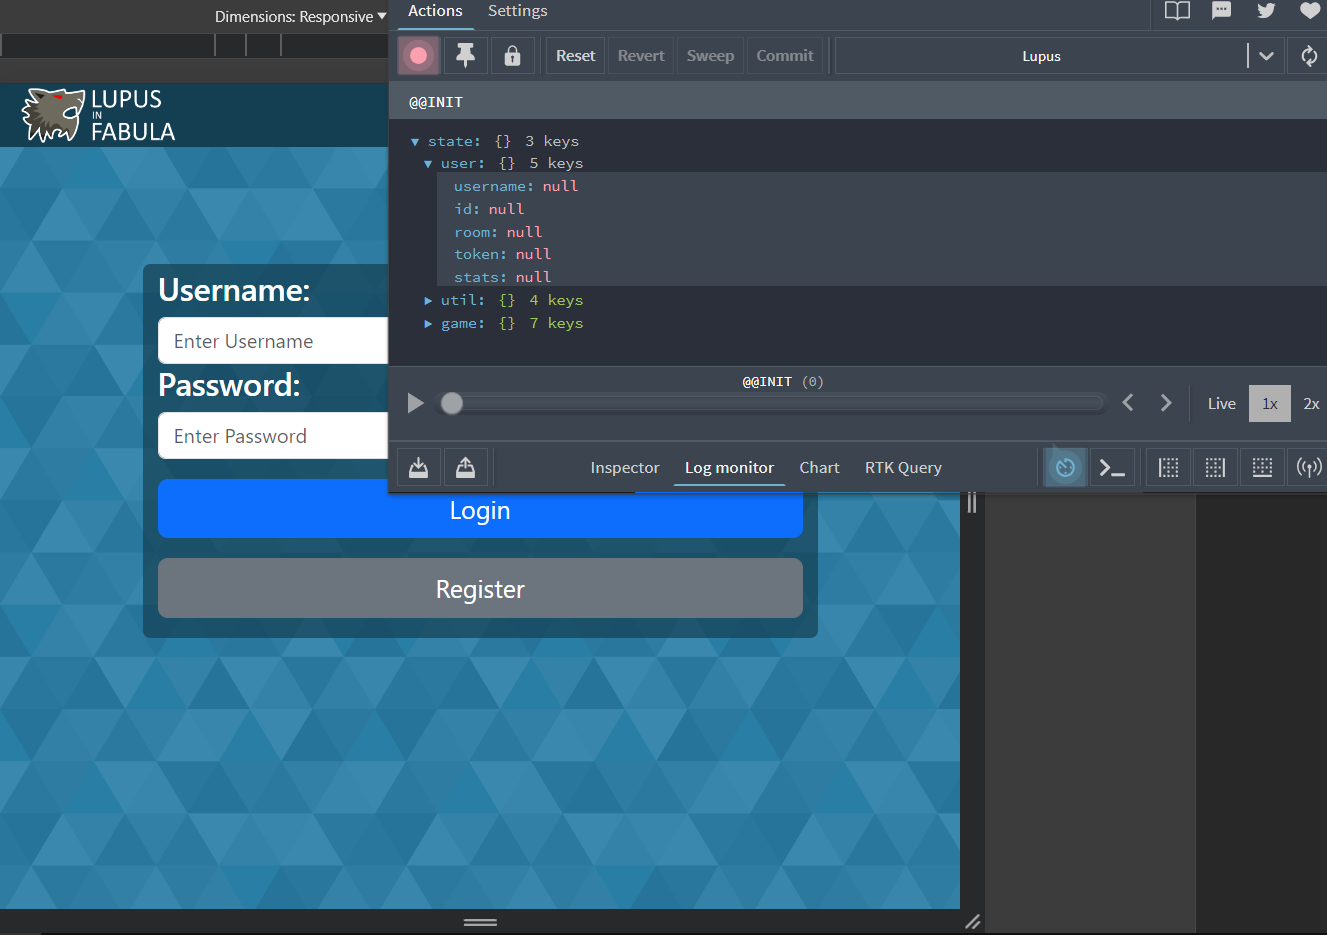
\includegraphics[width=0.9\textwidth]{img/redux_devtools_usage.png}
\caption{Redux DevTools in uso}
\label{fig:reduxDevTools}
\end{figure}

Per lo sviluppo di questo progetto è stata utilizzata l'estensione messa a disposizione per Chrome, come mostrato nell figura \ref{fig:reduxDevTools}, nella quale è possibile vedere lo stato in tempo reale di Redux.

\begin{figure}[H]
\centering
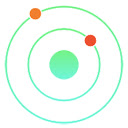
\includegraphics[width=0.3\textwidth]{img/logos/redux_devtool.jpg}
\caption{Redux DevTools logo}
\label{fig:reduxDevToolsLogo}
\end{figure}


\section{Axe DevTools}

Per testare aspetti di accessibilità sono stati invece utilizzati gli strumenti messi a disposizione da axe DevTools \cite{dequeDevToolsDeveloper}.
Questi tools permettono, sempre attraverso un'estensione disponibile per il browser Chrome, di analizzare vari aspetti di accessibilità relativi ad una specifica pagina web o ad una sua sottoparte. 

L'utilizzo dei tools è visibile nella figura \ref{fig:axeDevTools}, nella quale si può inoltre osservare la struttura di suddivisione utilizzata per attribuire un livello di gravità al problema riscontrato.


\begin{figure}[H]
\centering
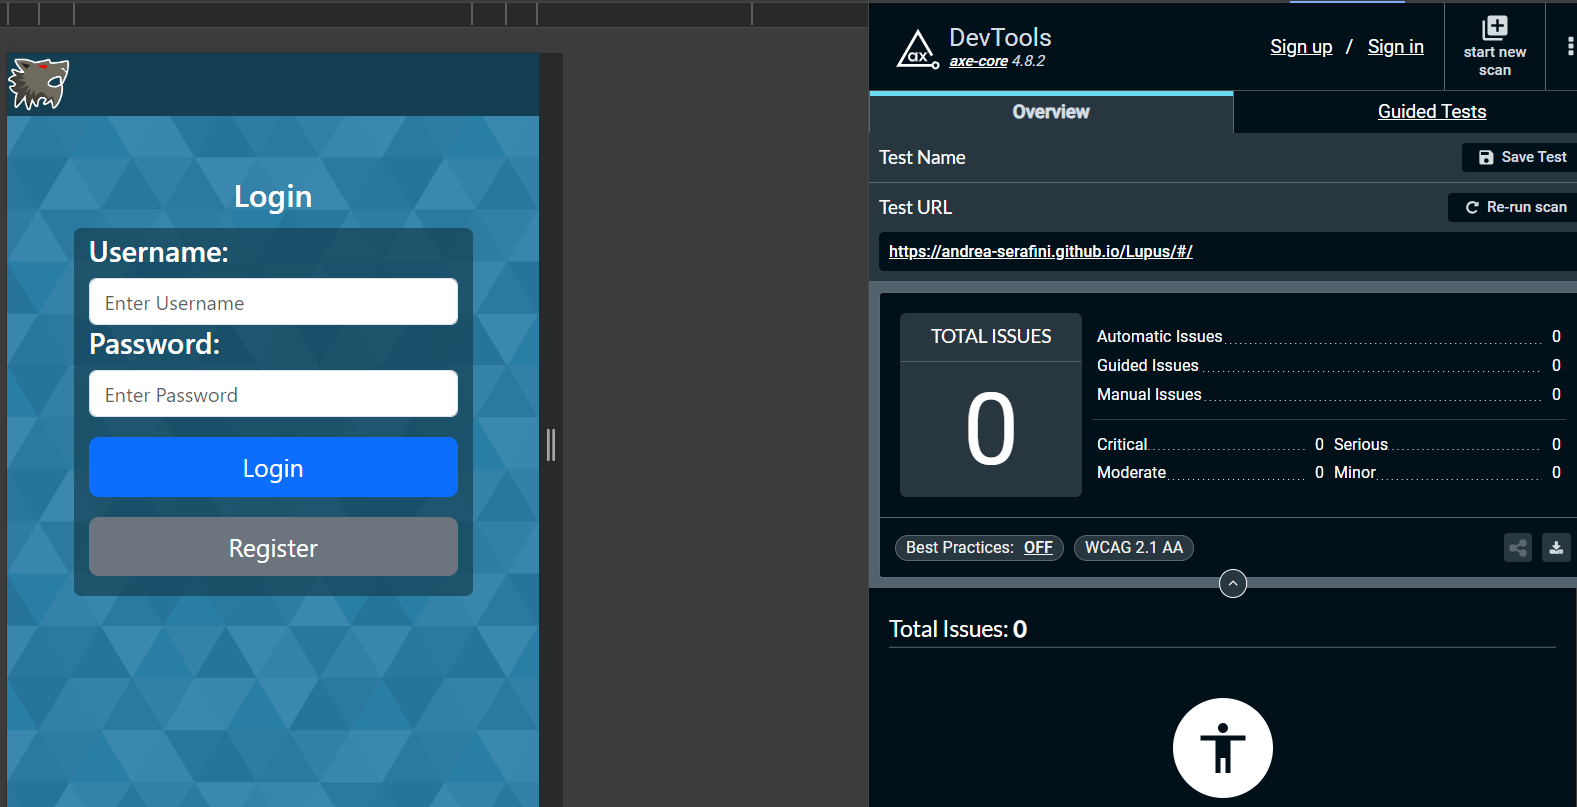
\includegraphics[width=\textwidth]{img/axe_devtools_usage.png}
\caption{Axe DevTools in uso}
\label{fig:axeDevTools}
\end{figure}

Il set di tool di cui ci siamo serviti per monitorare ed eventualmente correggere questioni riguardanti l'accessibilità nel presente applicativo. Axe DevTools è un insieme di strumenti leader del settore, che permette tramite un'estensione installabile direttamente su browser di ispezionare una pagina web o sottoparti di essa allo scopo di individuare problemi di accessibilità. Il tool poi procede con il suddividere i problemi in varie categorie a seconda della gravità dei problemi eventualmente riscontrati:

\begin{figure}[H]
\centering

\includegraphics[width=0.4\textwidth]{img/logos/axeDevtools_logo.png}
\caption{Axe DevTools logo}
\label{fig:axeDevToolsLogo}
\end{figure}


\section{Lighthouse}
Lighthouse è uno strumento automatizzato completamente open-source pensato per migliorare le prestazioni, la qualità e la correttezza delle applicazioni Web \cite{githubLighthouse}.

Durante il controllo di una pagina, questo tool esegue una serie di test sulla pagina e quindi genera un rapporto sul rendimento della pagina, visibile nella figura \ref{fig:lighthouseReport}. Da qui è possibile utilizzare eventuali test falliti come indicatori di quali azioni si possano intraprendere per migliorare la propria applicazione.

\begin{figure}[H]
\centering
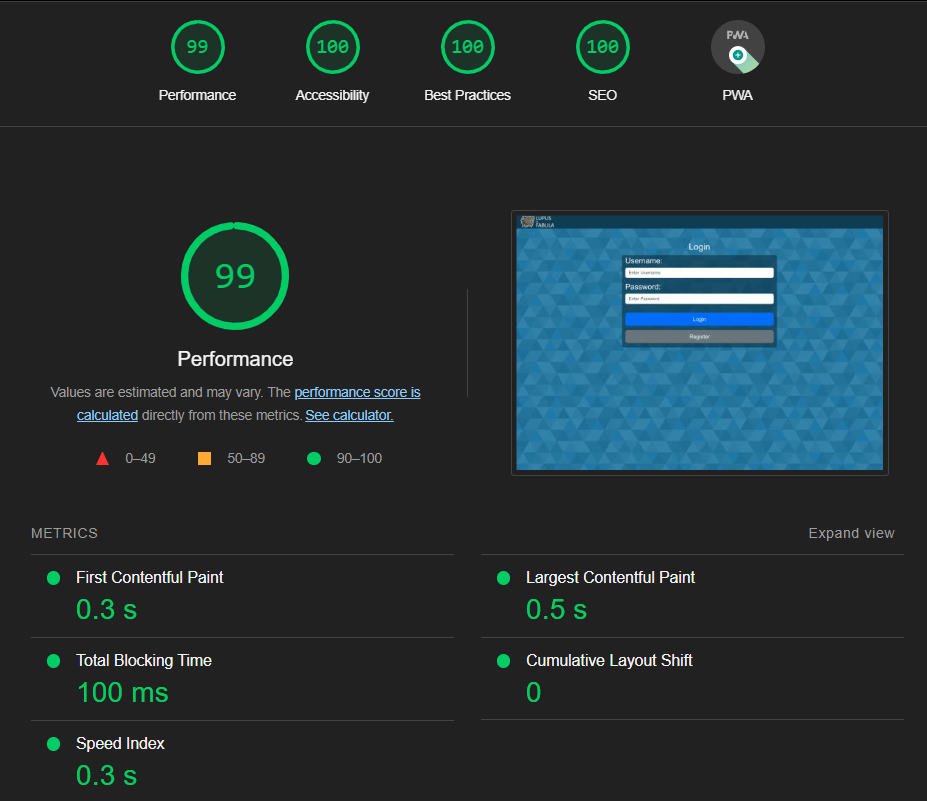
\includegraphics[width=0.8\textwidth]{img/lighthouse_usage.png}
\caption{Lighthouse in uso}
\label{fig:lighthouseReport}
\end{figure}

\begin{figure}[H]
\centering

\includegraphics[width=0.3\textwidth]{img/logos/lighthouse_logo.png}
\caption{Lighthouse logo}
\label{fig:lighthouseLogo}
\end{figure}

\chapter{Deployment}
In questo capitolo verranno illustrate le modalità e gli strumenti utilizzati per effettuare il deploy dell'applicazione sviluppata.

\section{Node-NPM}
La prima modalità utilizzata per effettuare il deploy del servizio è sta quella basata su \emph{Node} ed \emph{npm}. Per poter quindi eseguire questi step sarà necessario installare o verificare l'installazione dei seguenti componenti.
\begin{itemize}
    \item MongoDB
    \item Node
    \item npm
\end{itemize}
Per verificare l'installazione di MongoDB sarà sufficiente lanciare il comando \inlinecode{bash}{mongod -version}, nel caso non fosse presente bisognerà procedere ad installarlo. Analogamente con i comandi \inlinecode{bash}{node -v} e \inlinecode{bash}{npm -v} si verificherà la versione installata degli altri due.

Una volta che l'ambiente è stato correttamente impostato sarà sufficiente utilizzare \emph{git} per importare il progetto, oppure scaricarlo manualmente direttamente dalla pagina web del repository.

\subsection{Local}
Per le fasi di sviluppo il sistema è stato utilizzato in modalità locale, con l'obiettivo di verificarne il funzionamento in itinere. Per fare ciò è stato necessario avviare localmente le due componenti, server e client.

Per avviare il server dopo essersi spostati all'interno dell'omonima cartella con il terminale bisognerà eseguire i seguenti comandi:

\begin{lcverbatim}
    npm install
    set LUPUS_SERVER_PORT=8081
    node server.js
\end{lcverbatim}

Il primo si occuperà di installare tutte le dipendenze necessarie, mentre l'ultimo avvierà effettivamente il server. Per quanto riguarda invece il secondo comando mostrato, il suo utilizzo è opzionale in quanto all'interno del progetto la variabile d'ambiente riportata viene impostata di default al valore \emph{8080}, perciò l'utilizzo del comando si riduce al solo caso in cui sia necessario utilizzare una porta diversa.

Ora per avviare il client bisognerà analogamente da un nuovo terminale spostarsi nella cartella corretta, poi eseguire i seguenti comandi:

\begin{lcverbatim}
    npm install
    set REACT_APP_SERVER_PORT=8081
    npm run build
    serve -s build
\end{lcverbatim}

Dopo aver installato tutte le dipendenze sarà necessario eseguire il secondo comando per modificare la porta alla quale contattare il server solo nel caso si fosse modificata rispetto a quella di default \emph{8080}. I seguenti comandi si occuperanno di creare la build e rendere l'applicazione accessibile online come mostrato nella figura \ref{fig:serve}.

\begin{figure}[H]
\centering
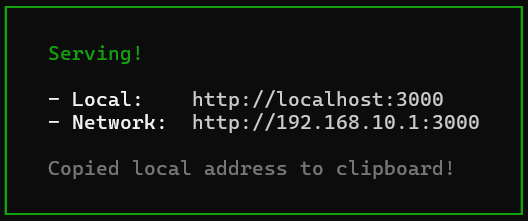
\includegraphics[width=0.7\textwidth]{img/serve.png}
\caption{Output del comando serve}
\label{fig:serve}
\end{figure}

\subsection{Distributed}
Per la fase di test eseguita in maniera distribuita è stato necessario introdurre alcuni strumenti ulteriori. Per raggiungere questo obiettivo sono stati quindi utilizzati anche:
\begin{itemize}
    \item Ngrok\cite{ngrok}
    \item GitHub Pages\cite{gitHubreactghpages}
\end{itemize}

Il primo è un reverse proxy server cross-platform con cui è possibile esporre un server locale, collocato dietro NAT, e firewall alla rete Internet tramite secure tunnel. Dopo aver creato un dominio dalla dashboard messa a disposizione sul loro sito utilizzando il comando  
\begin{lcverbatim}
    ngrok tunnel --label edge=edghts_*** http://localhost:8080
\end{lcverbatim}
sarà possibile connettersi al server sulla macchina locale anche dalla rete esterna all'indirizzo \inlinecode{bash}{wise-resolved-wasp.ngrok-free.app}.

Il codice del client dovrà poi essere modificato per sostituire l'indirizzo \emph{localhost} con quello pubblico. Effettuata la sostituzione è stato sfruttato il servizio offerto da GitHub, ovvero GitHub Pages.

Pages permette di fare hosting di un sito web direttamente dal repository del progetto. Avendo aggiunto anche \inlinecode{bash}{"deploy": "gh-pages -d build"} agli script sarà possibile eseguire il comando
\begin{lcverbatim}
    npm run deploy -- -m "Deploy message"
\end{lcverbatim}
per effettuare la build del client e pushare la nuova versione dell'applicazione.

Dopo aver svolto tutti gli step sarà possibile accedere al sito all'indirizzo
\begin{lcverbatim}
    https://andrea-serafini.github.io/Lupus/
\end{lcverbatim}
per poter utilizzare il sistema collegandosi da remoto al server locale.

\section{Docker}
Per effettuare un deployment semplificato e indipendente dall'architettura della quale si dispone sono stati impostati i file necessari per l'utilizzo di Docker.
Una volta installata e avviata l'applicazione di Docker i comandi da eseguire da linea di comando saranno:
\begin{lcverbatim}
#Per avviare
    docker compose up --build

#Per terminare
    docker compose down
\end{lcverbatim}

La struttura del progetto e dei conseguenti file \emph{docker-compose} permette sia di avviare tutti i container insieme, che di avviare in maniera separata il client e la coppia server-database.
\section{Conclusioni}

\subsection{Sviluppi futuri}
In futuro ampliando e approfondendo il progetto i punti salienti che presentano possibilità di ulteriori sviluppi sono risultati:

\begin{itemize}
    \item \textbf{Applicazione mobile:} come era stato ipotizzato in fase di definizione delle specifiche di progetto sarebbe interessante, oltre che utile per migliorarne la fruibilità, sviluppare un'applicazione mobile che faccia uso di librerie specifiche.
    \item \textbf{Comunicazione interna:} attualmente il sistema prevede che per apprezzare al meglio il gioco implementato gli utenti si ritrovino nello stesso luogo, o che utilizzino sistemi alternativi di comunicazione, come ad esempio Discord. In futuro sfruttando le capacità di PeerJS sarebbe interessante aggiungere la possibilità di comunicare all'interno della lobby, testualmente, con un canale audio, o addirittura video.
\end{itemize}
\subsection{Nozioni apprese}

Lo sviluppo di questo progetto ha permesso di approfondire, e familiarizzare con, i framework e i tool utilizzati, oltre che apprendere attraverso tentativi ed errori quali fossero le metodologie migliori per impostare un lavoro di questo tipo.

Il risultato finale ottenuto rispetta tutti i requisiti fondamentali definiti in fase di analisi e proposta di progetto, oltre che tutte le aspettative dal punto di vista di usabilità e funzionalità del sistema. Dopo aver effettuato test con amici e colleghi non solo il livello di implementazione è stato ritenuto più che soddisfacente, ma anche l'idea alla base della digitalizzazione del gioco ha riscosso molto successo, con numerose richieste per una futura release così da poter continuare a utilizzarlo.

I problemi riscontrati durante lo sviluppo hanno a volte rappresentato sfide importanti, soprattutto non avendo la possibilità di confrontarsi con un gruppo, ma per ognuno è stata trovata una soluzione o una via alternativa che nel complesso ho sempre ritenuto all'altezza delle personali aspettative.


\appendix
\chapter{Desktop screenshots}\label{appendix:desktop}

\begin{figure}[H]
\centering
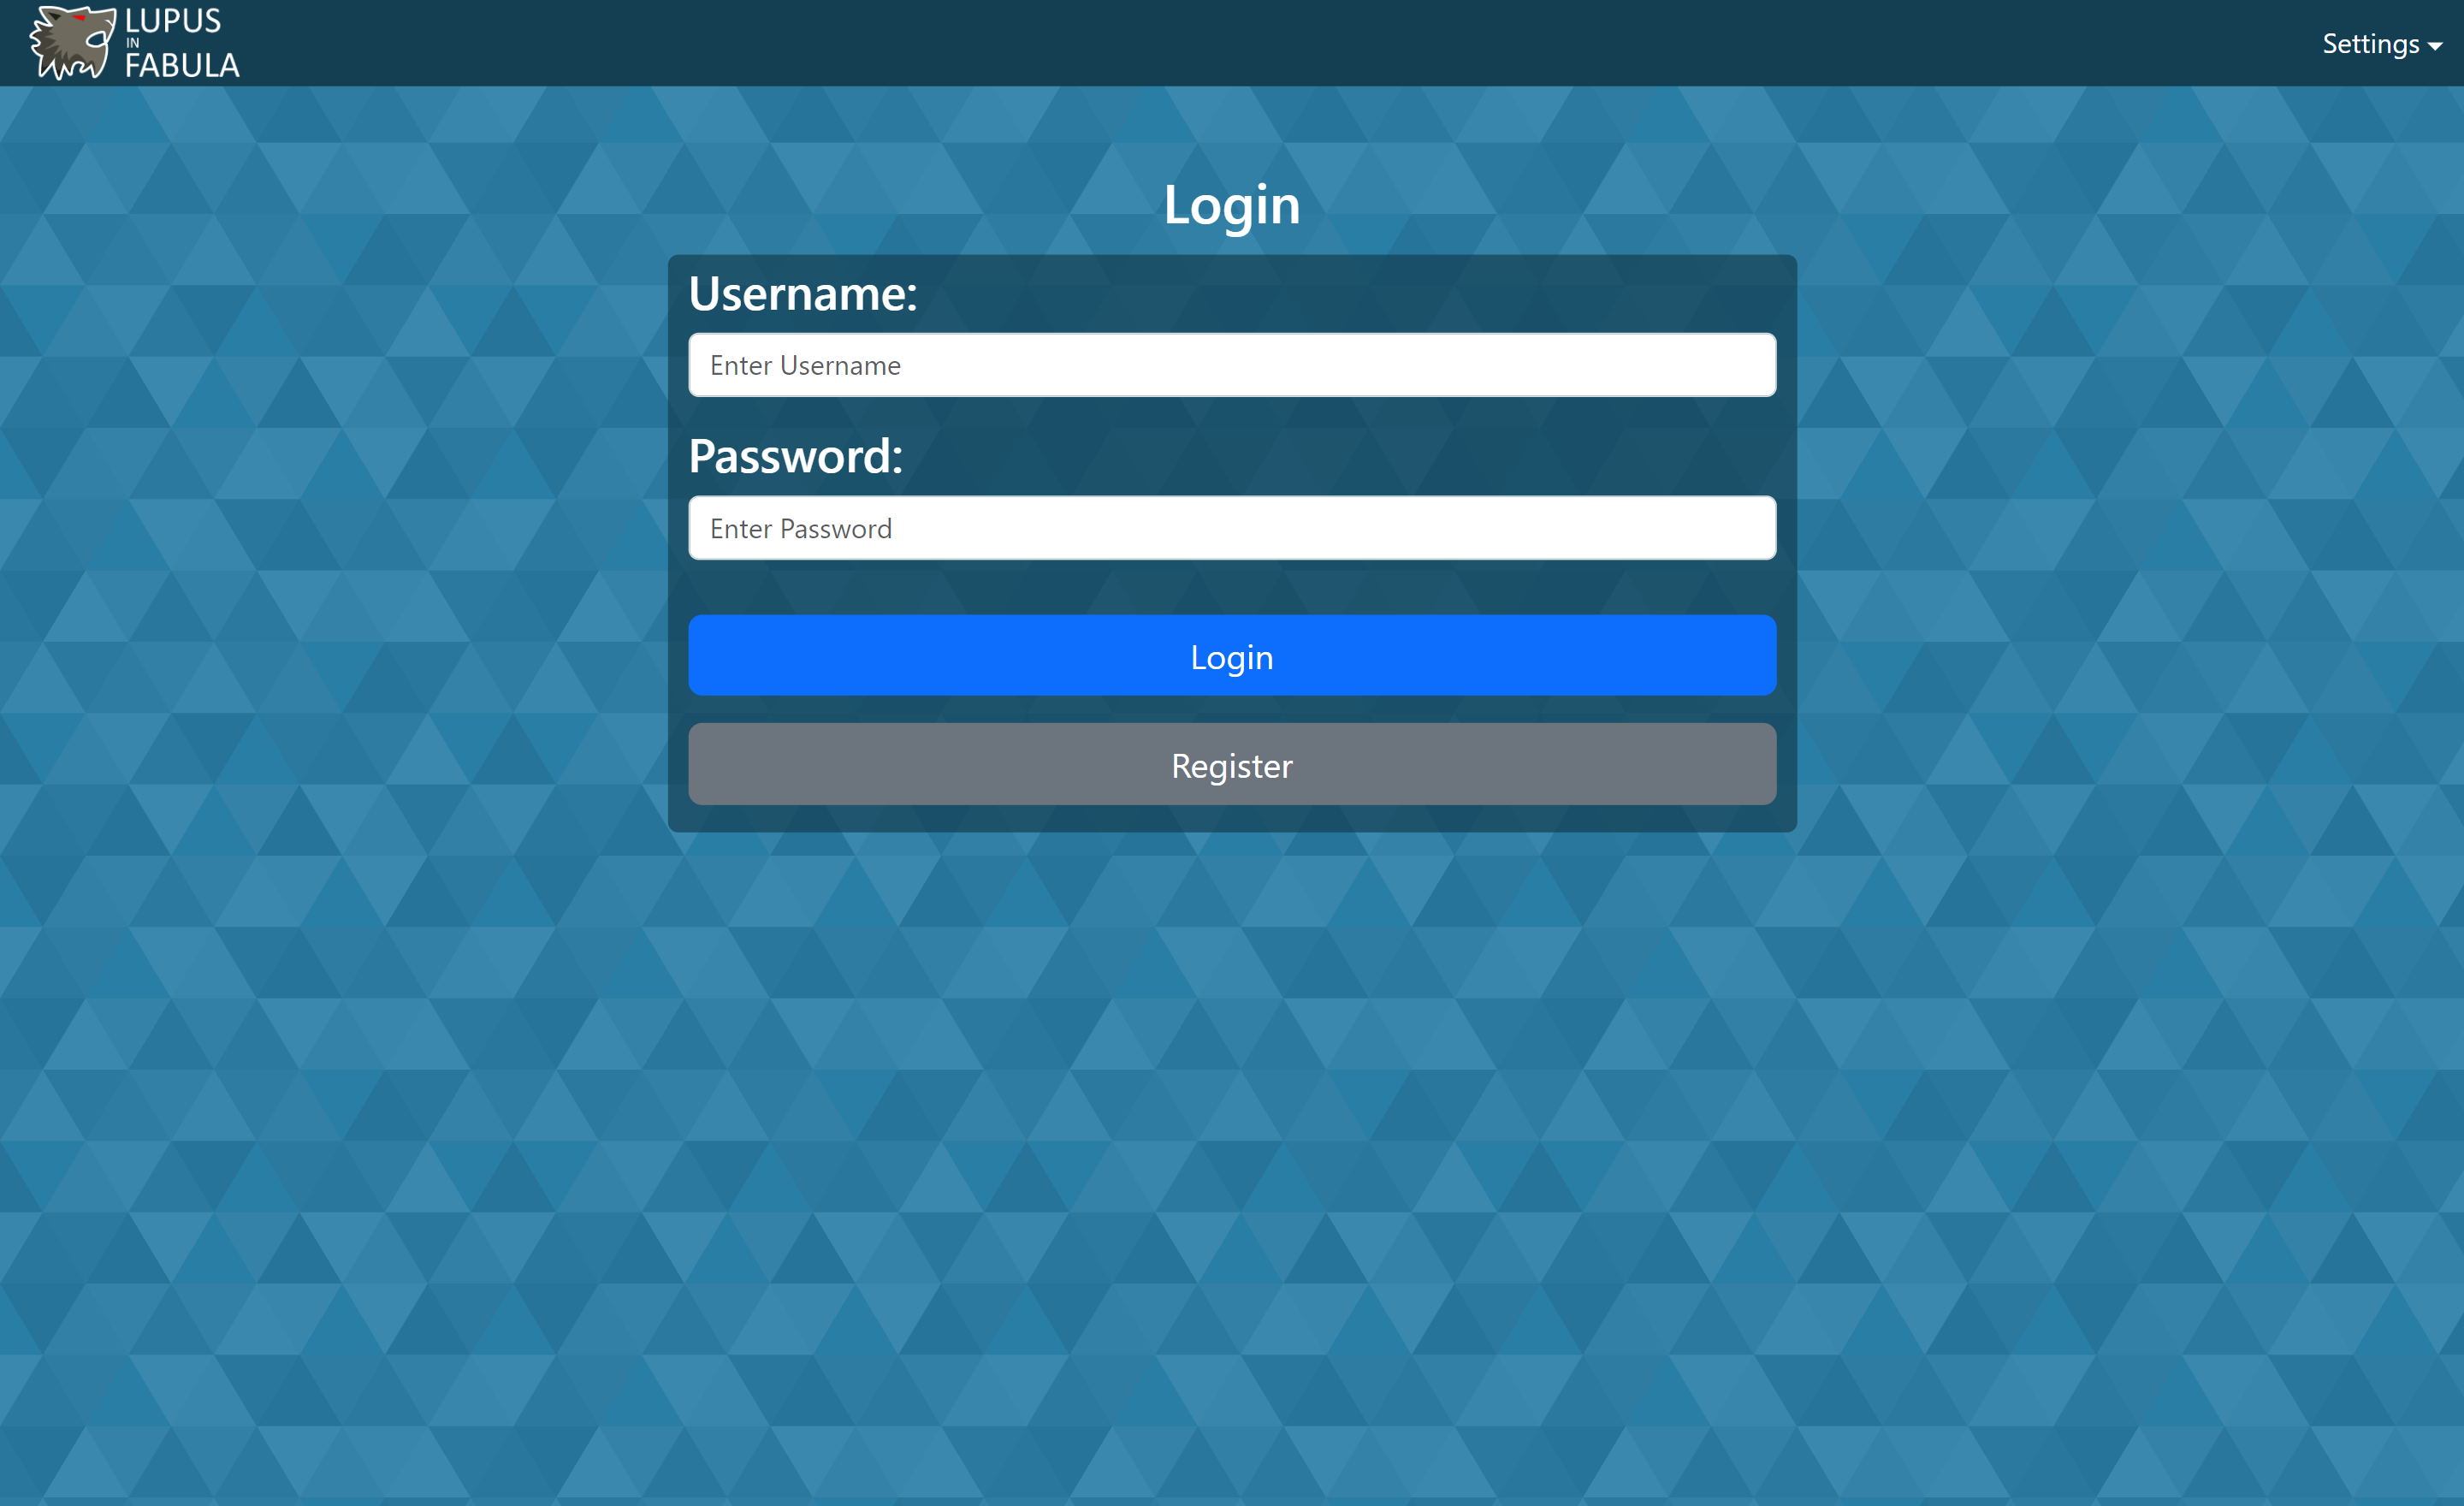
\includegraphics[width=\textwidth]{img/screen/desktop/login_desktop.png}
\caption{Schermata di autenticazione}
\label{fig:login_desktop}
\end{figure}

\begin{figure}[H]
\centering
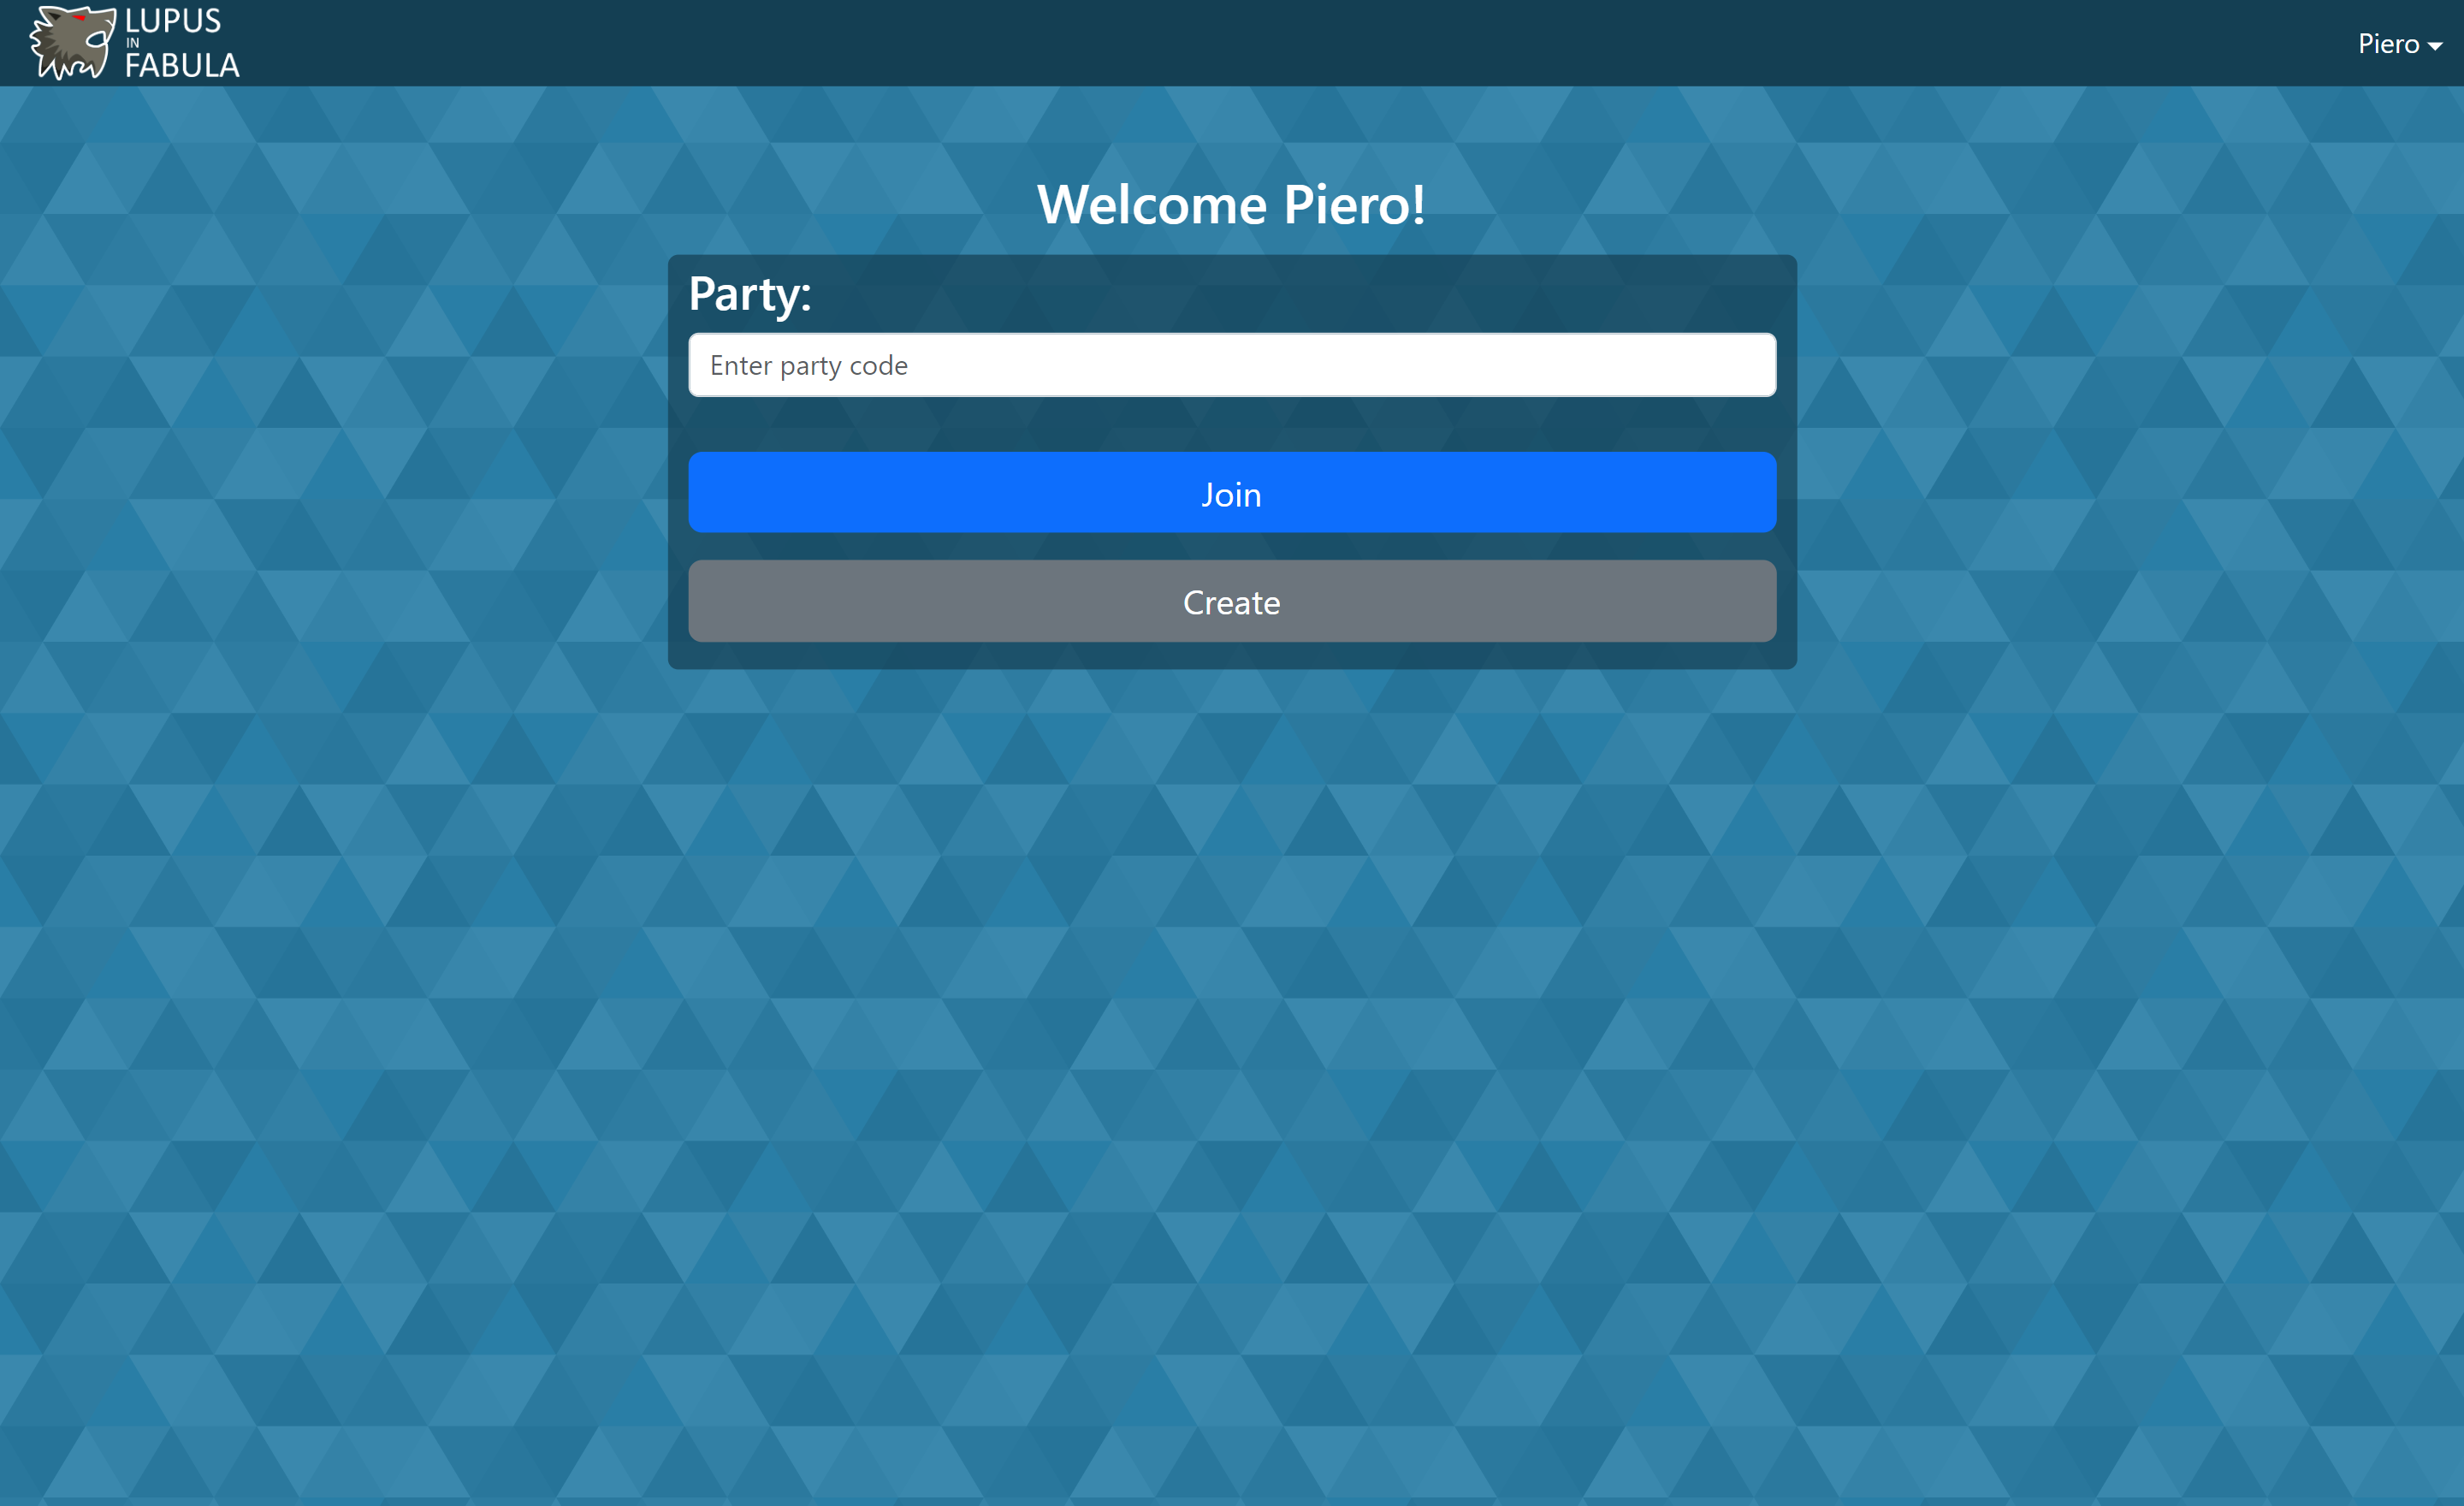
\includegraphics[width=\textwidth]{img/screen/desktop/party_desktop.png}
\caption{Schermata di selezione party}
\label{fig:party_desktop}
\end{figure}

\begin{figure}[H]
\centering
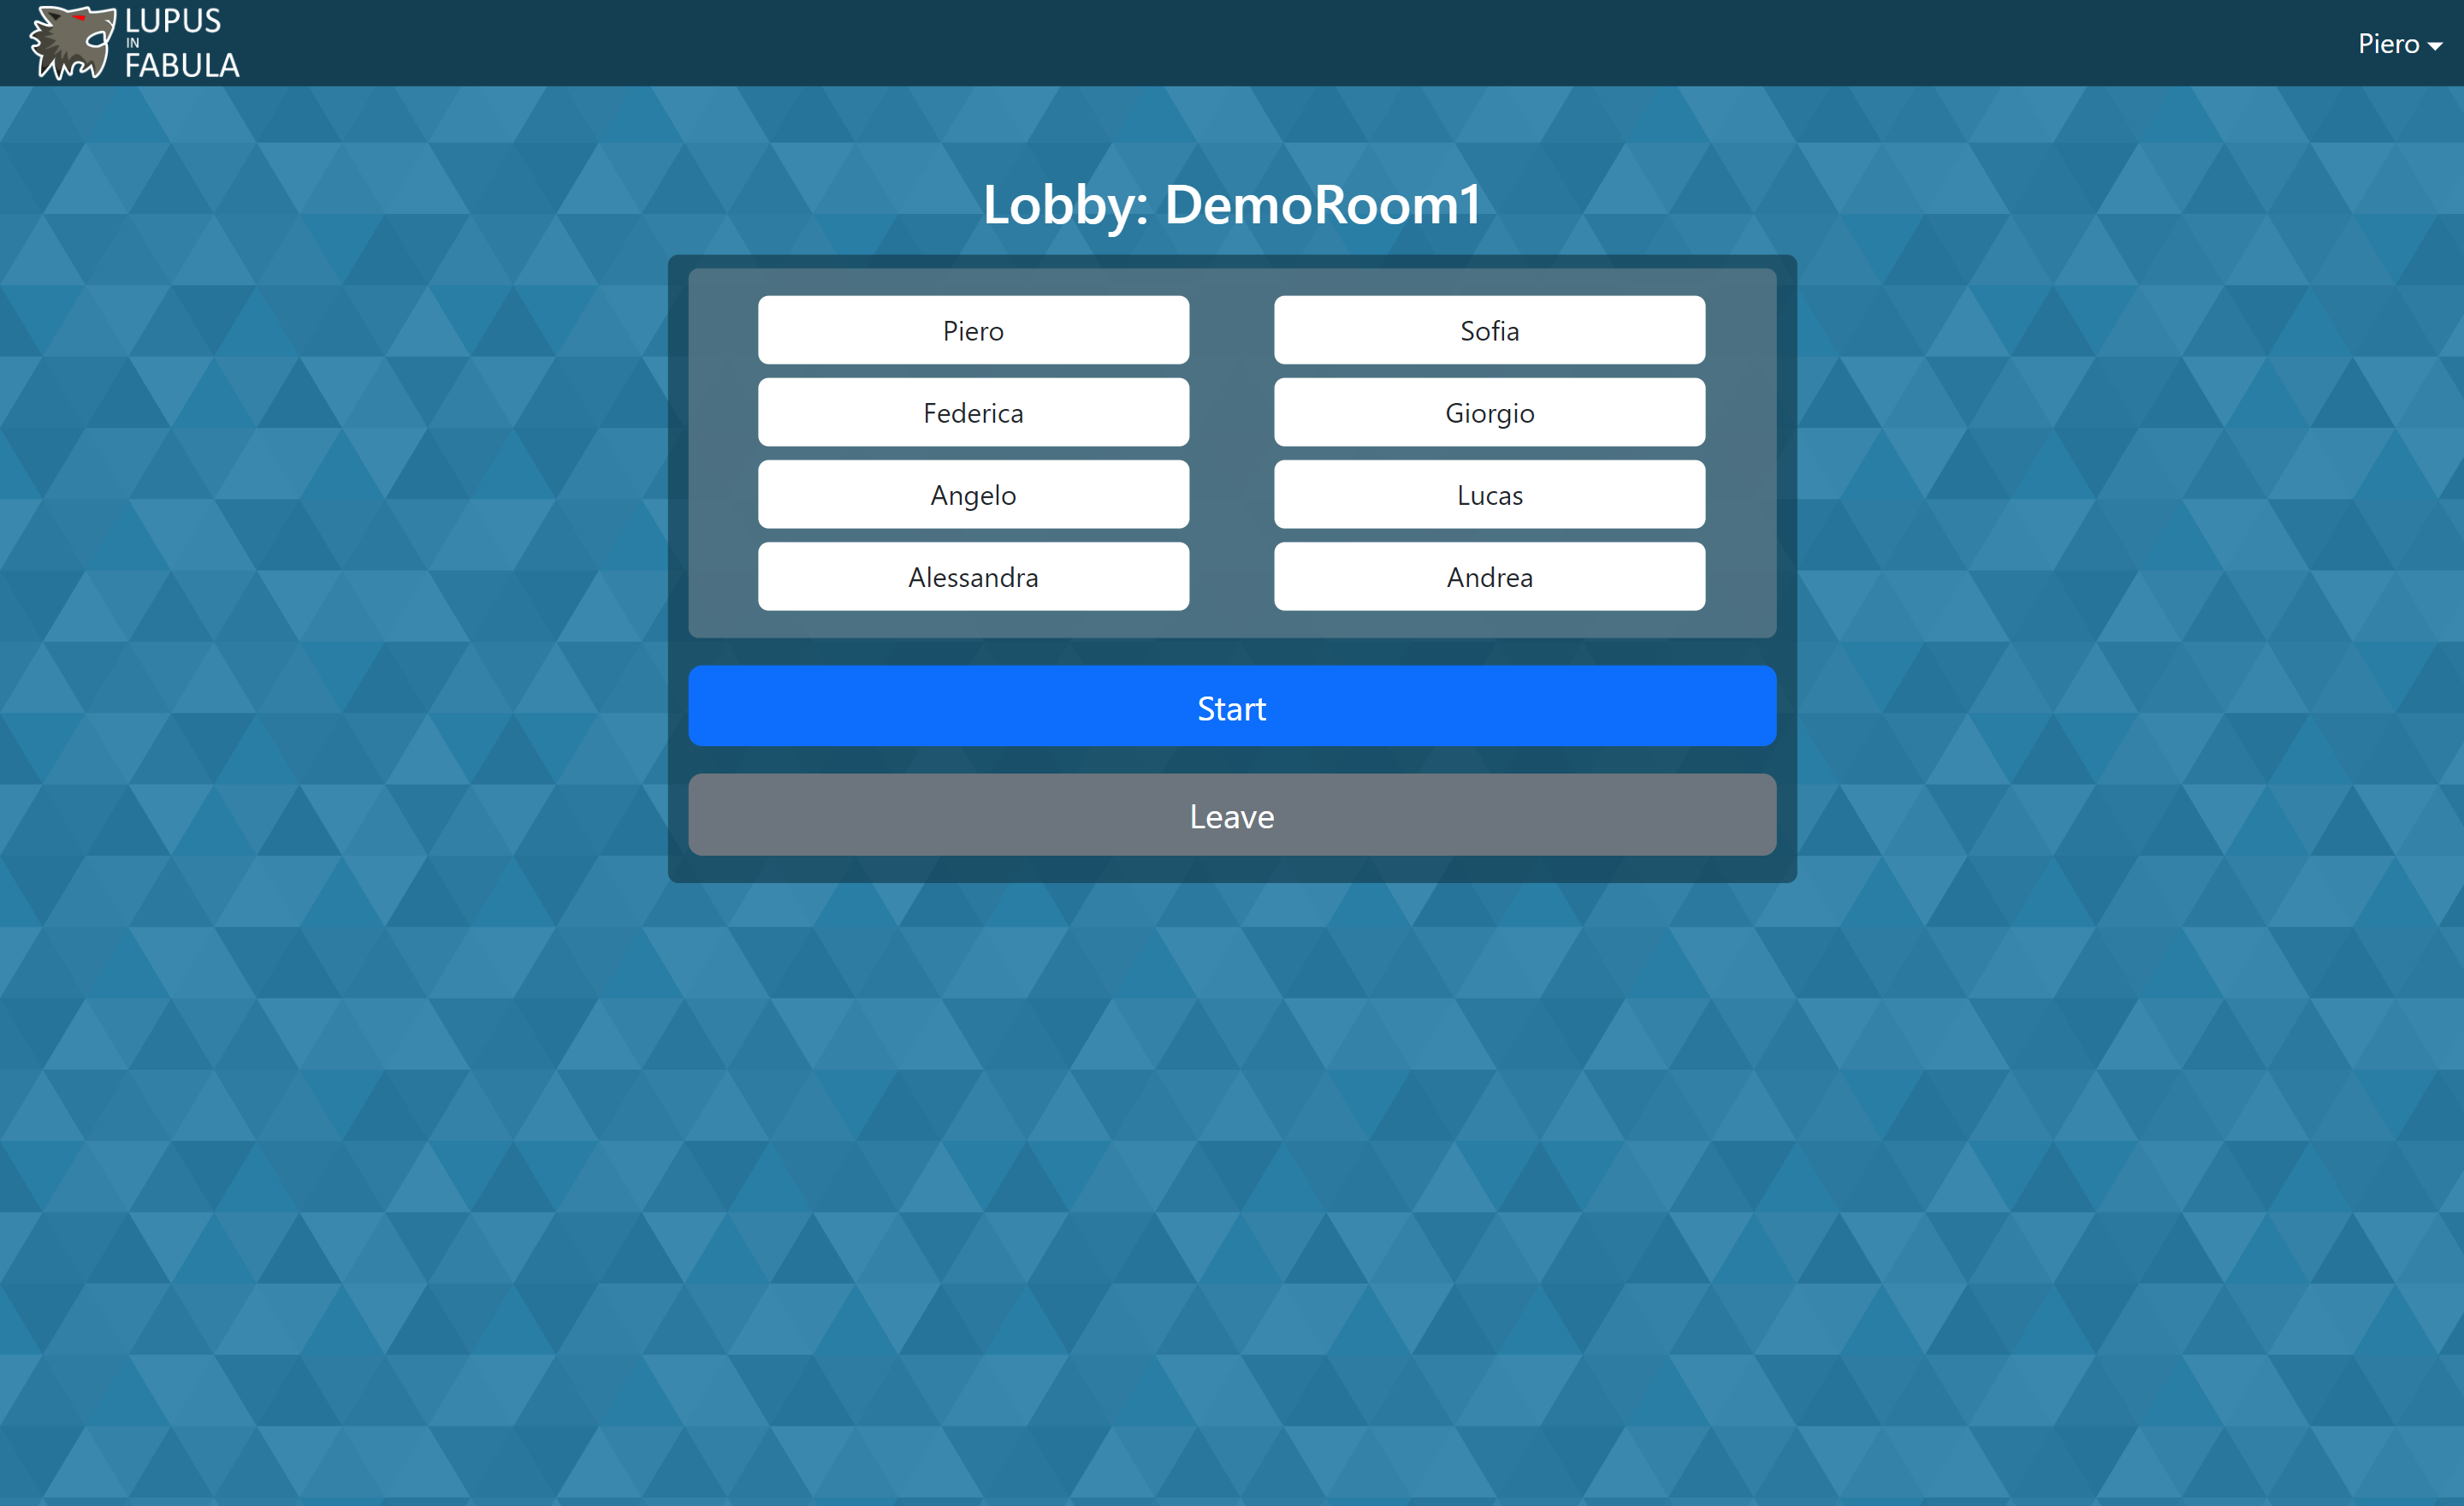
\includegraphics[width=\textwidth]{img/screen/desktop/lobby_desktop.png}
\caption{Schermata di lobby}
\label{fig:lobby_desktop}
\end{figure}

\begin{figure}[H]
\centering
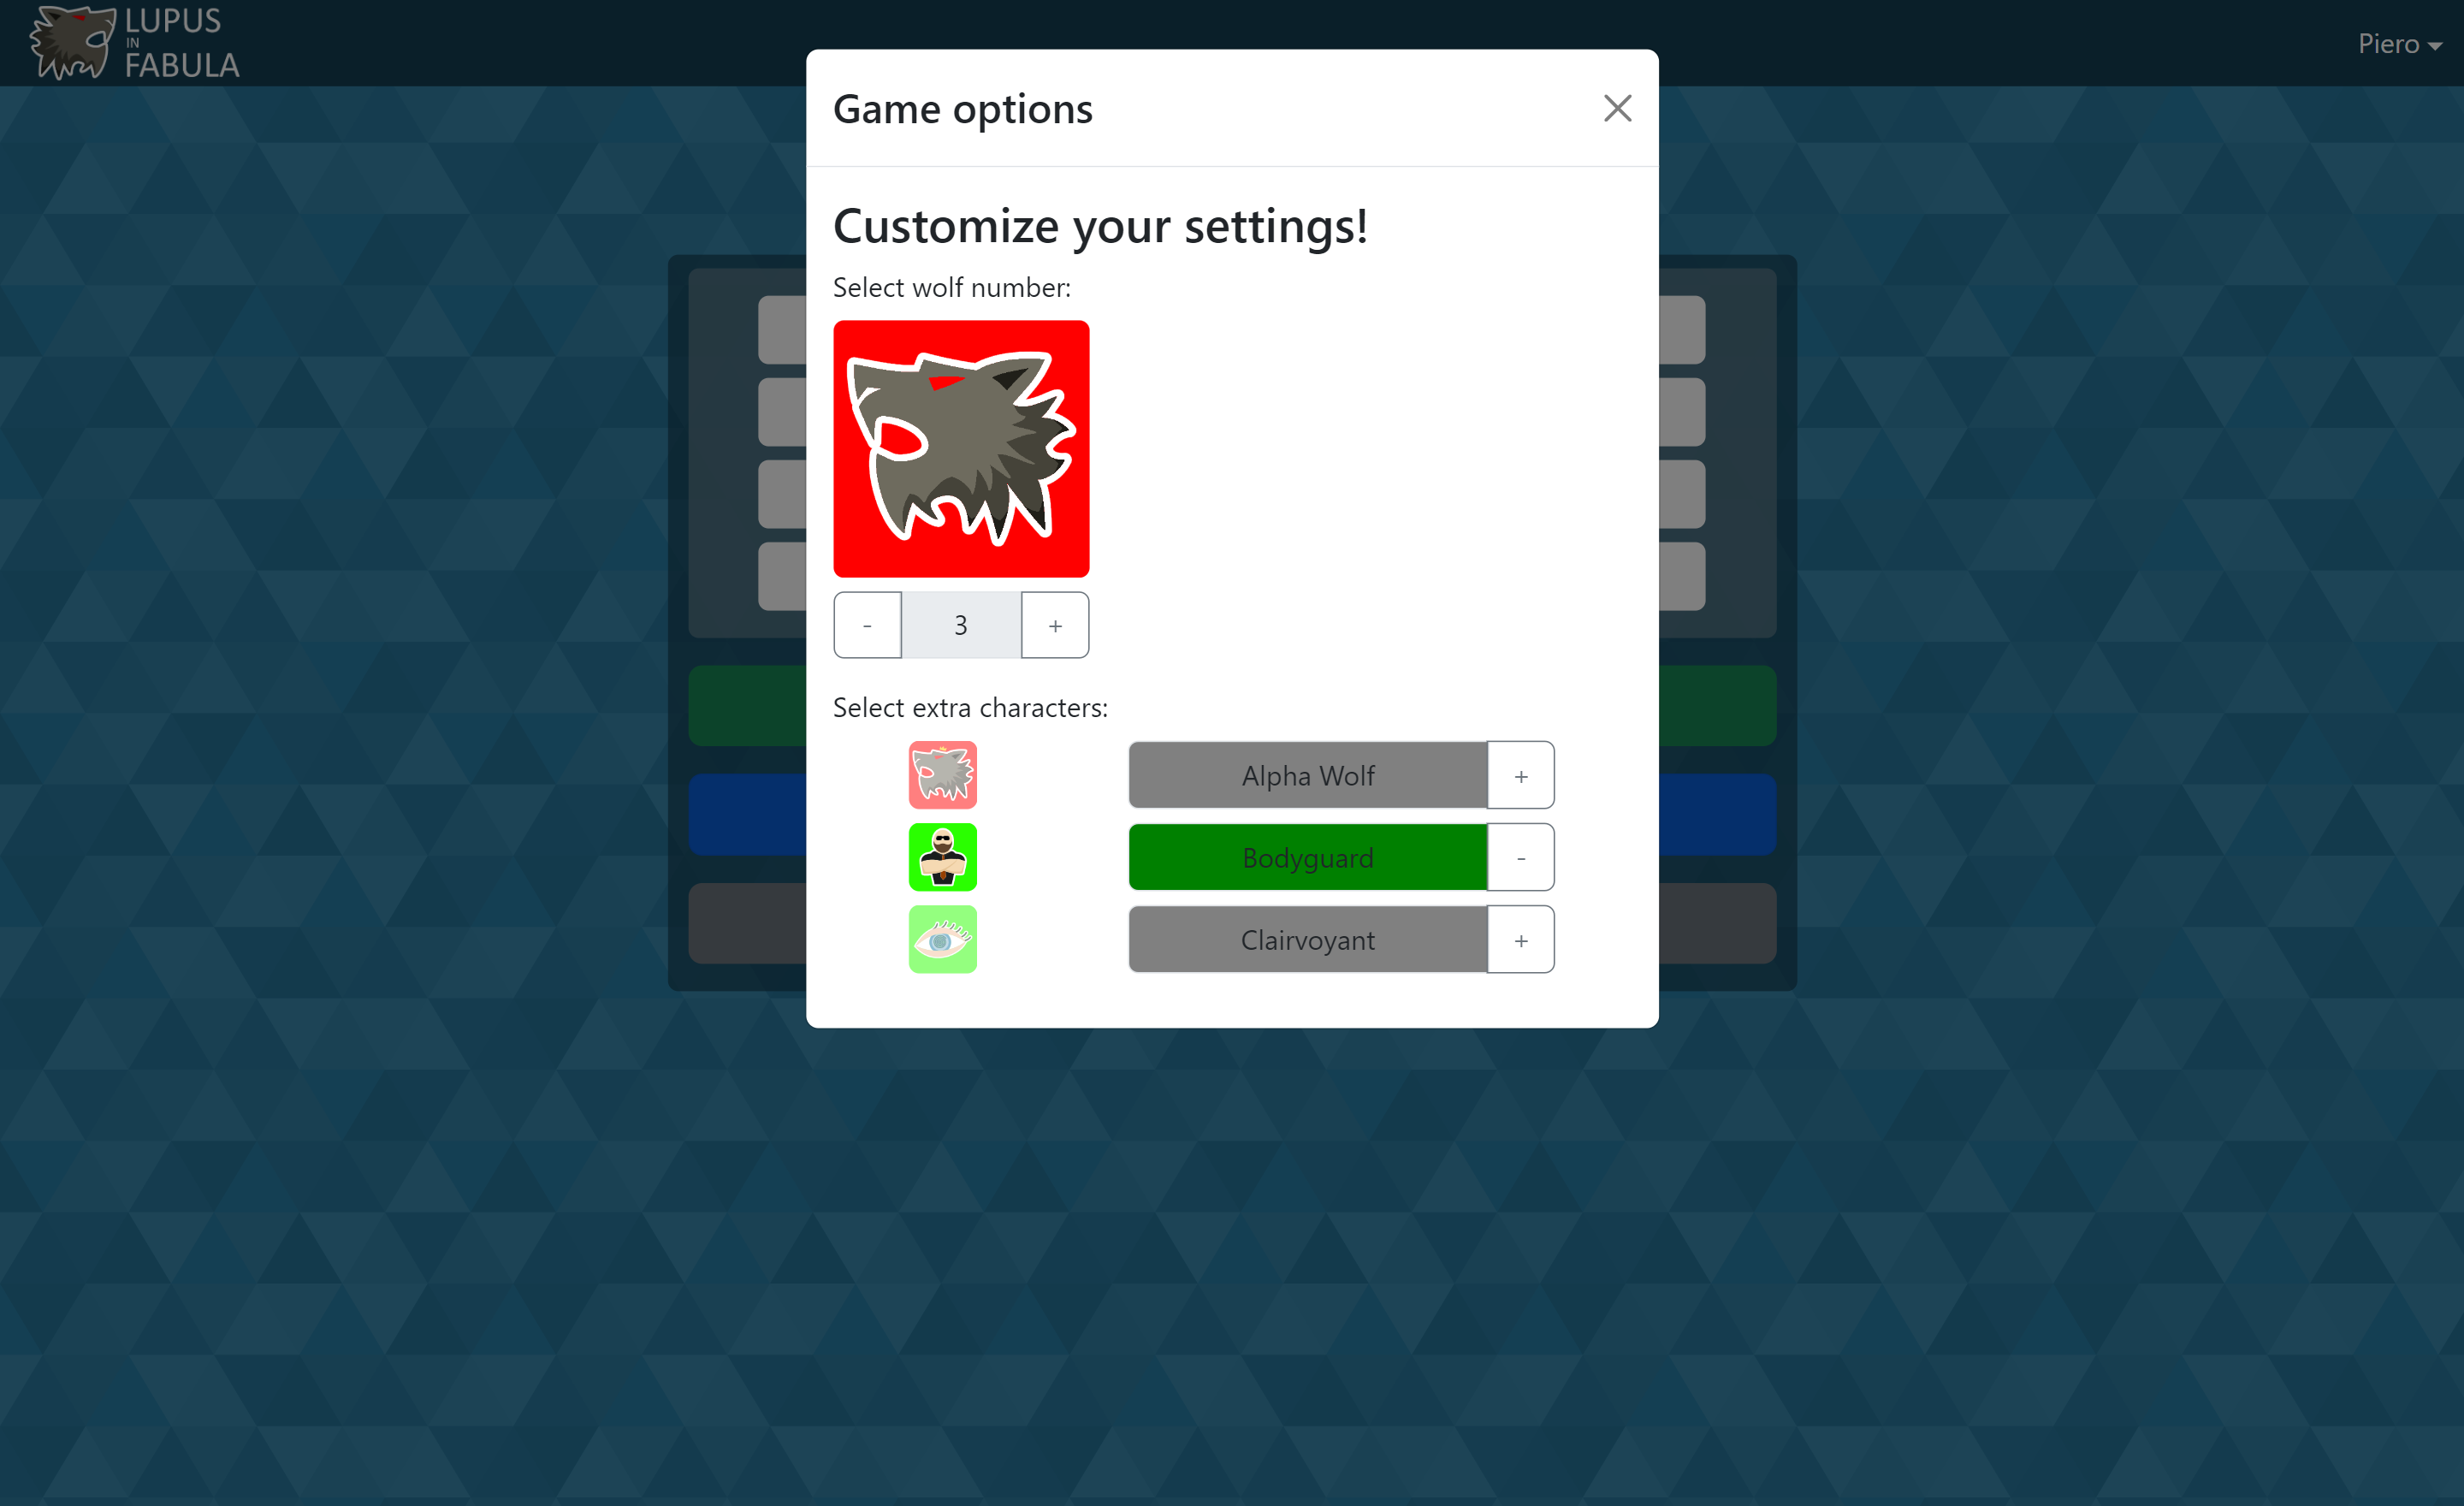
\includegraphics[width=\textwidth]{img/screen/desktop/option_desktop.png}
\caption{Schermata delle opzioni}
\label{fig:option_desktop}
\end{figure}

\begin{figure}[H]
\centering
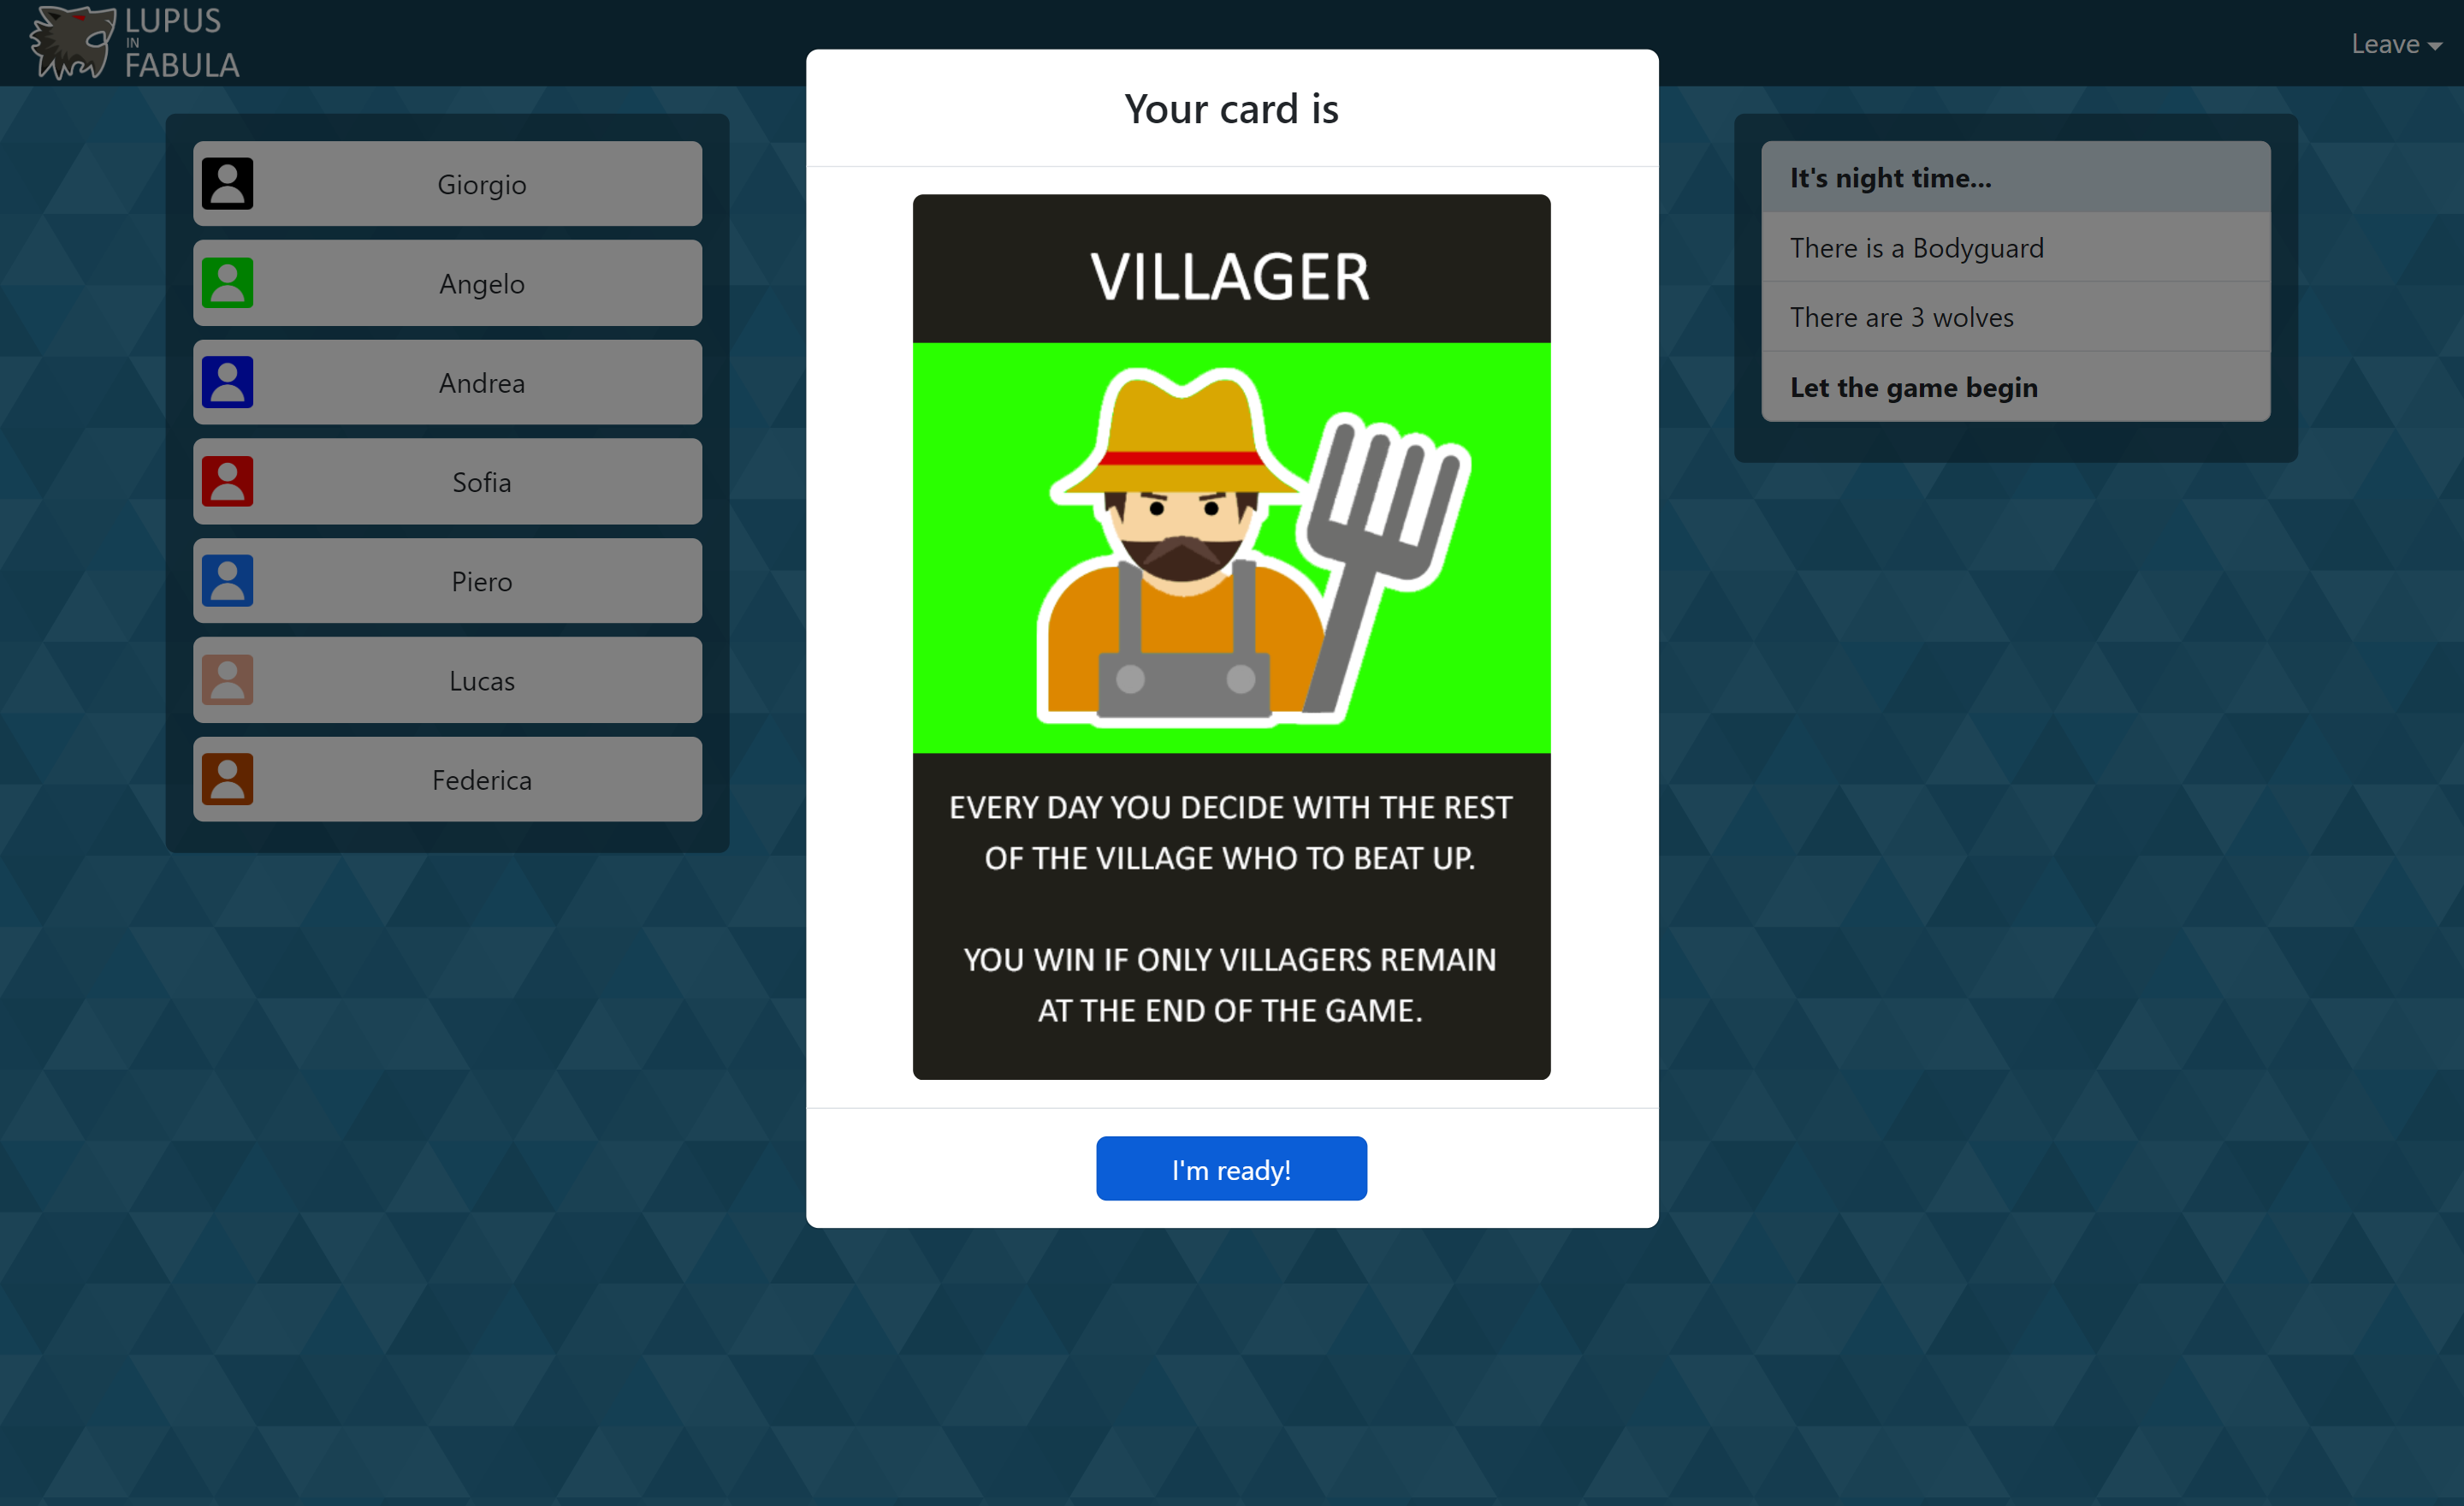
\includegraphics[width=\textwidth]{img/screen/desktop/card_desktop.png}
\caption{Schermata di inizio partita}
\label{fig:card_desktop}
\end{figure}

\begin{figure}[H]
\centering
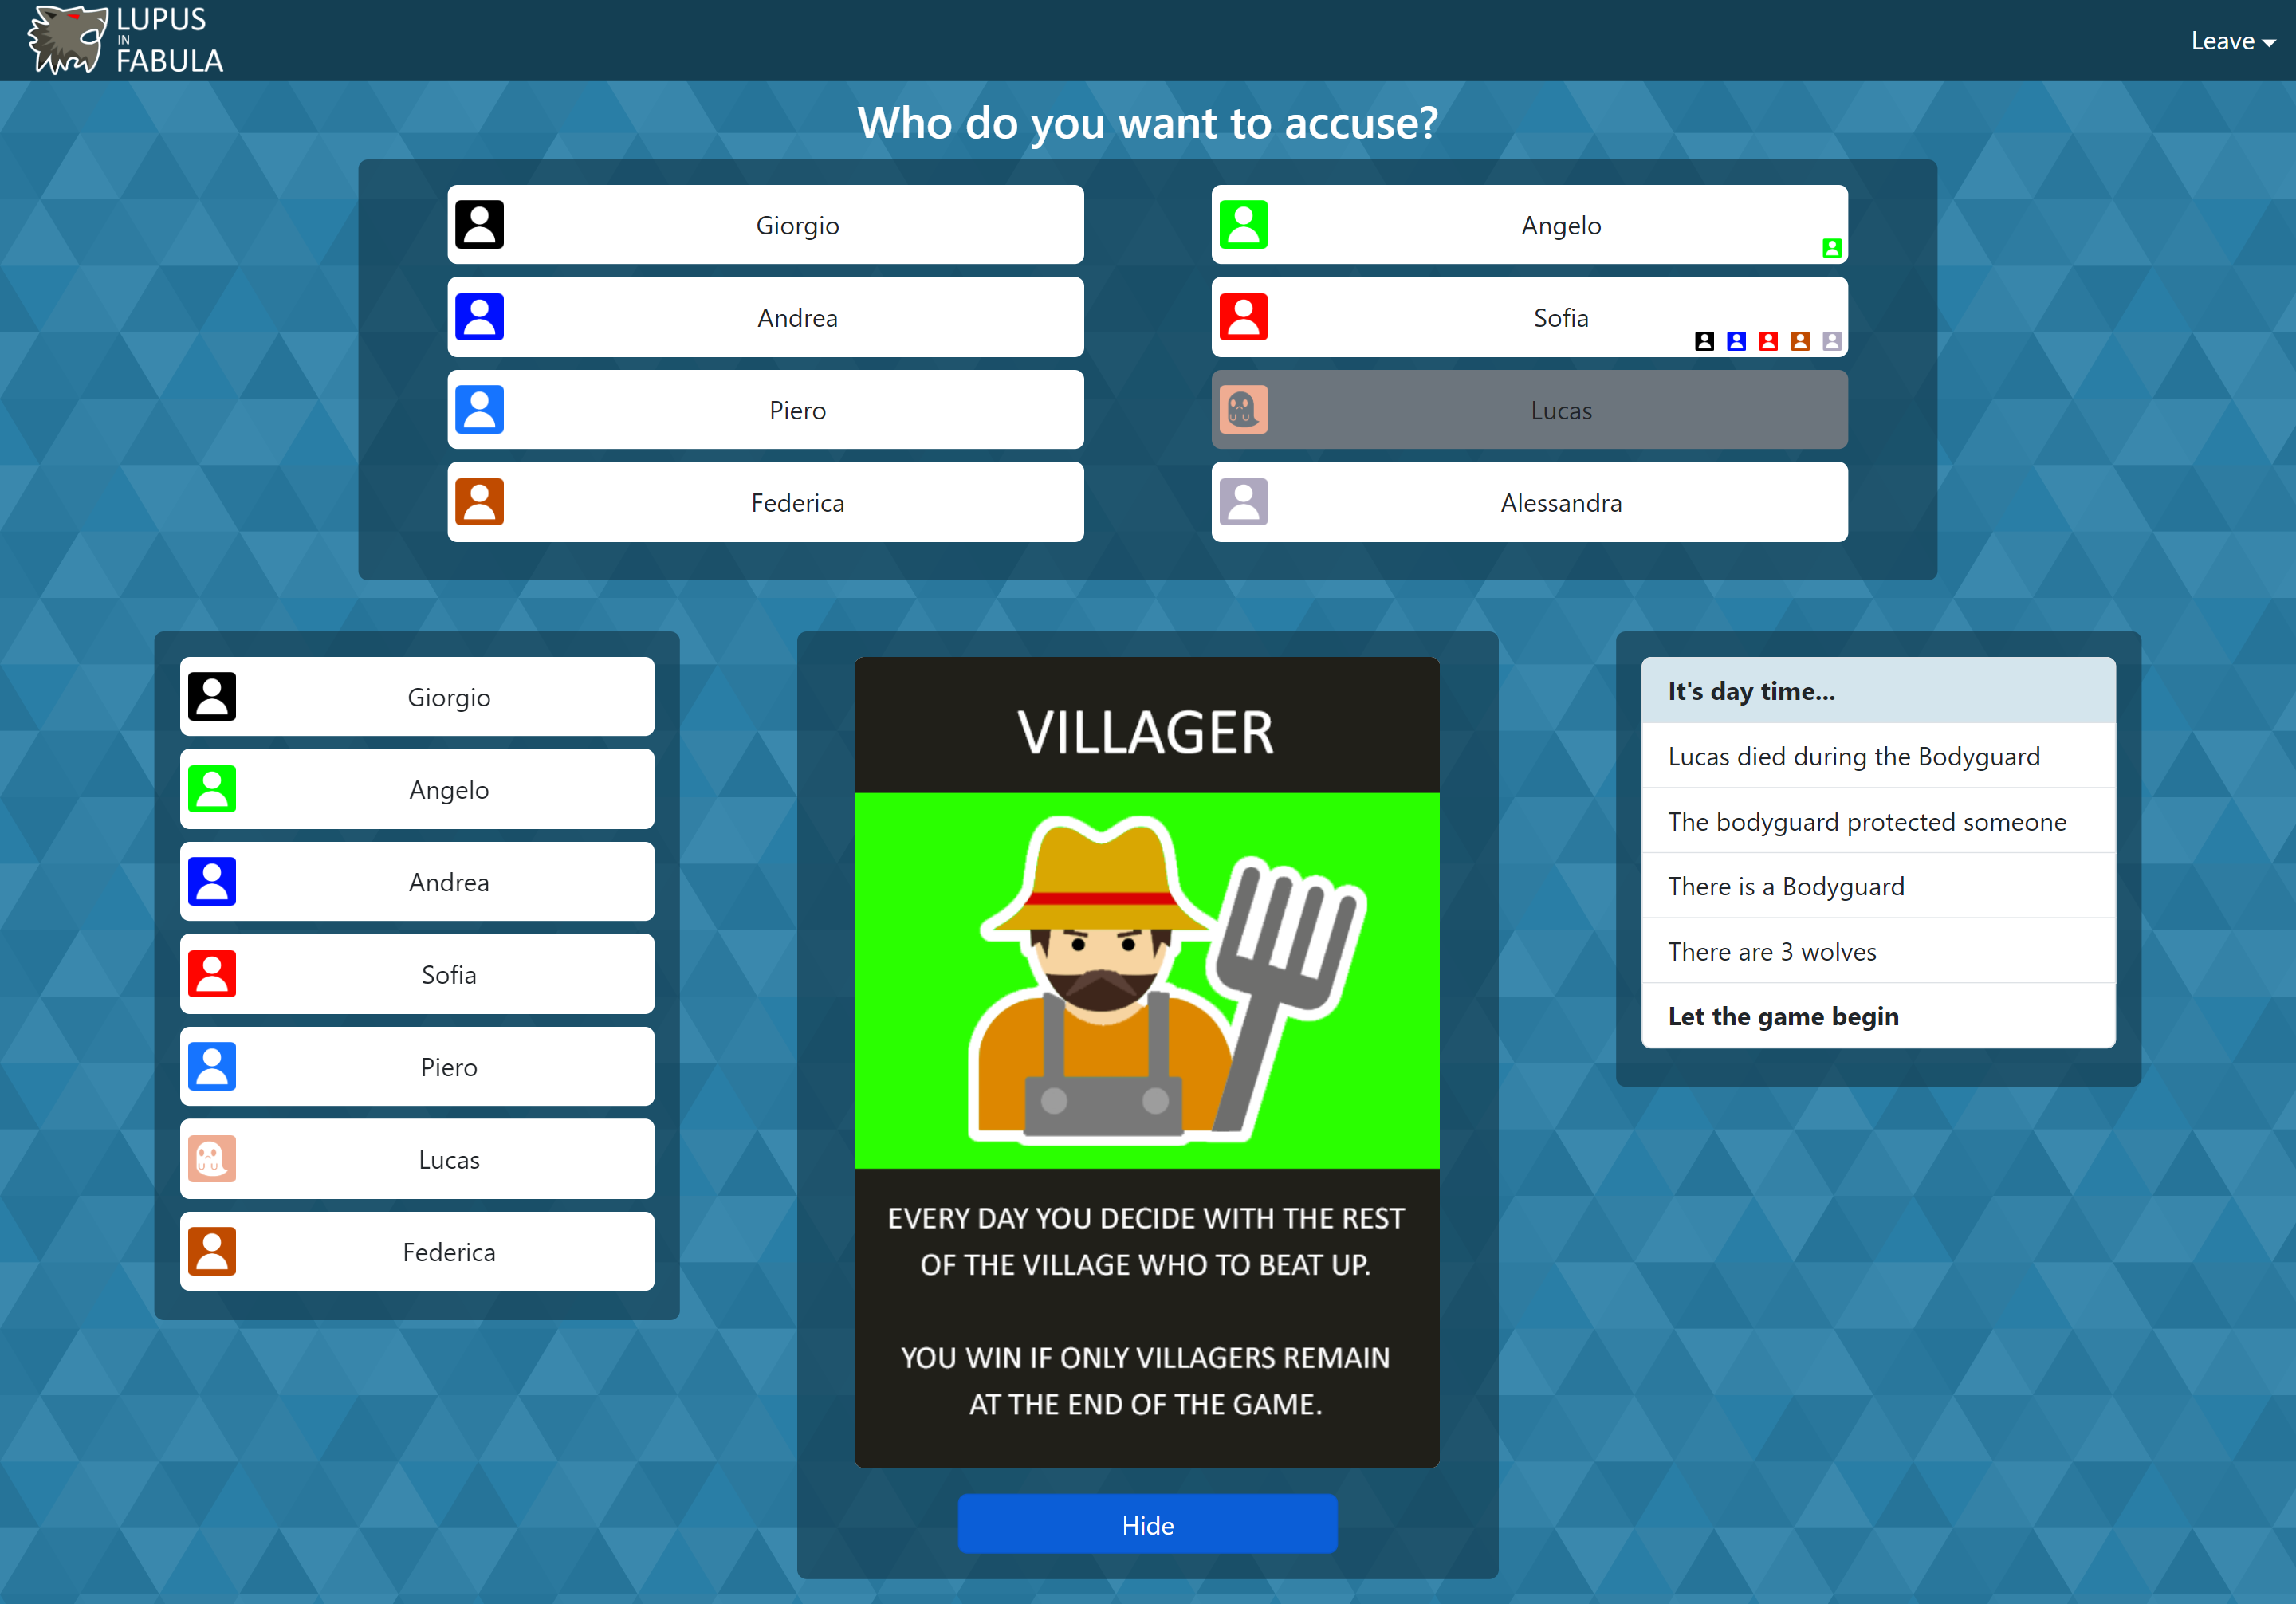
\includegraphics[width=\textwidth]{img/screen/desktop/accusation_desktop.png}
\caption{Schermata di turno di accusa}
\label{fig:accusation_desktop}
\end{figure}

\begin{figure}[H]
\centering
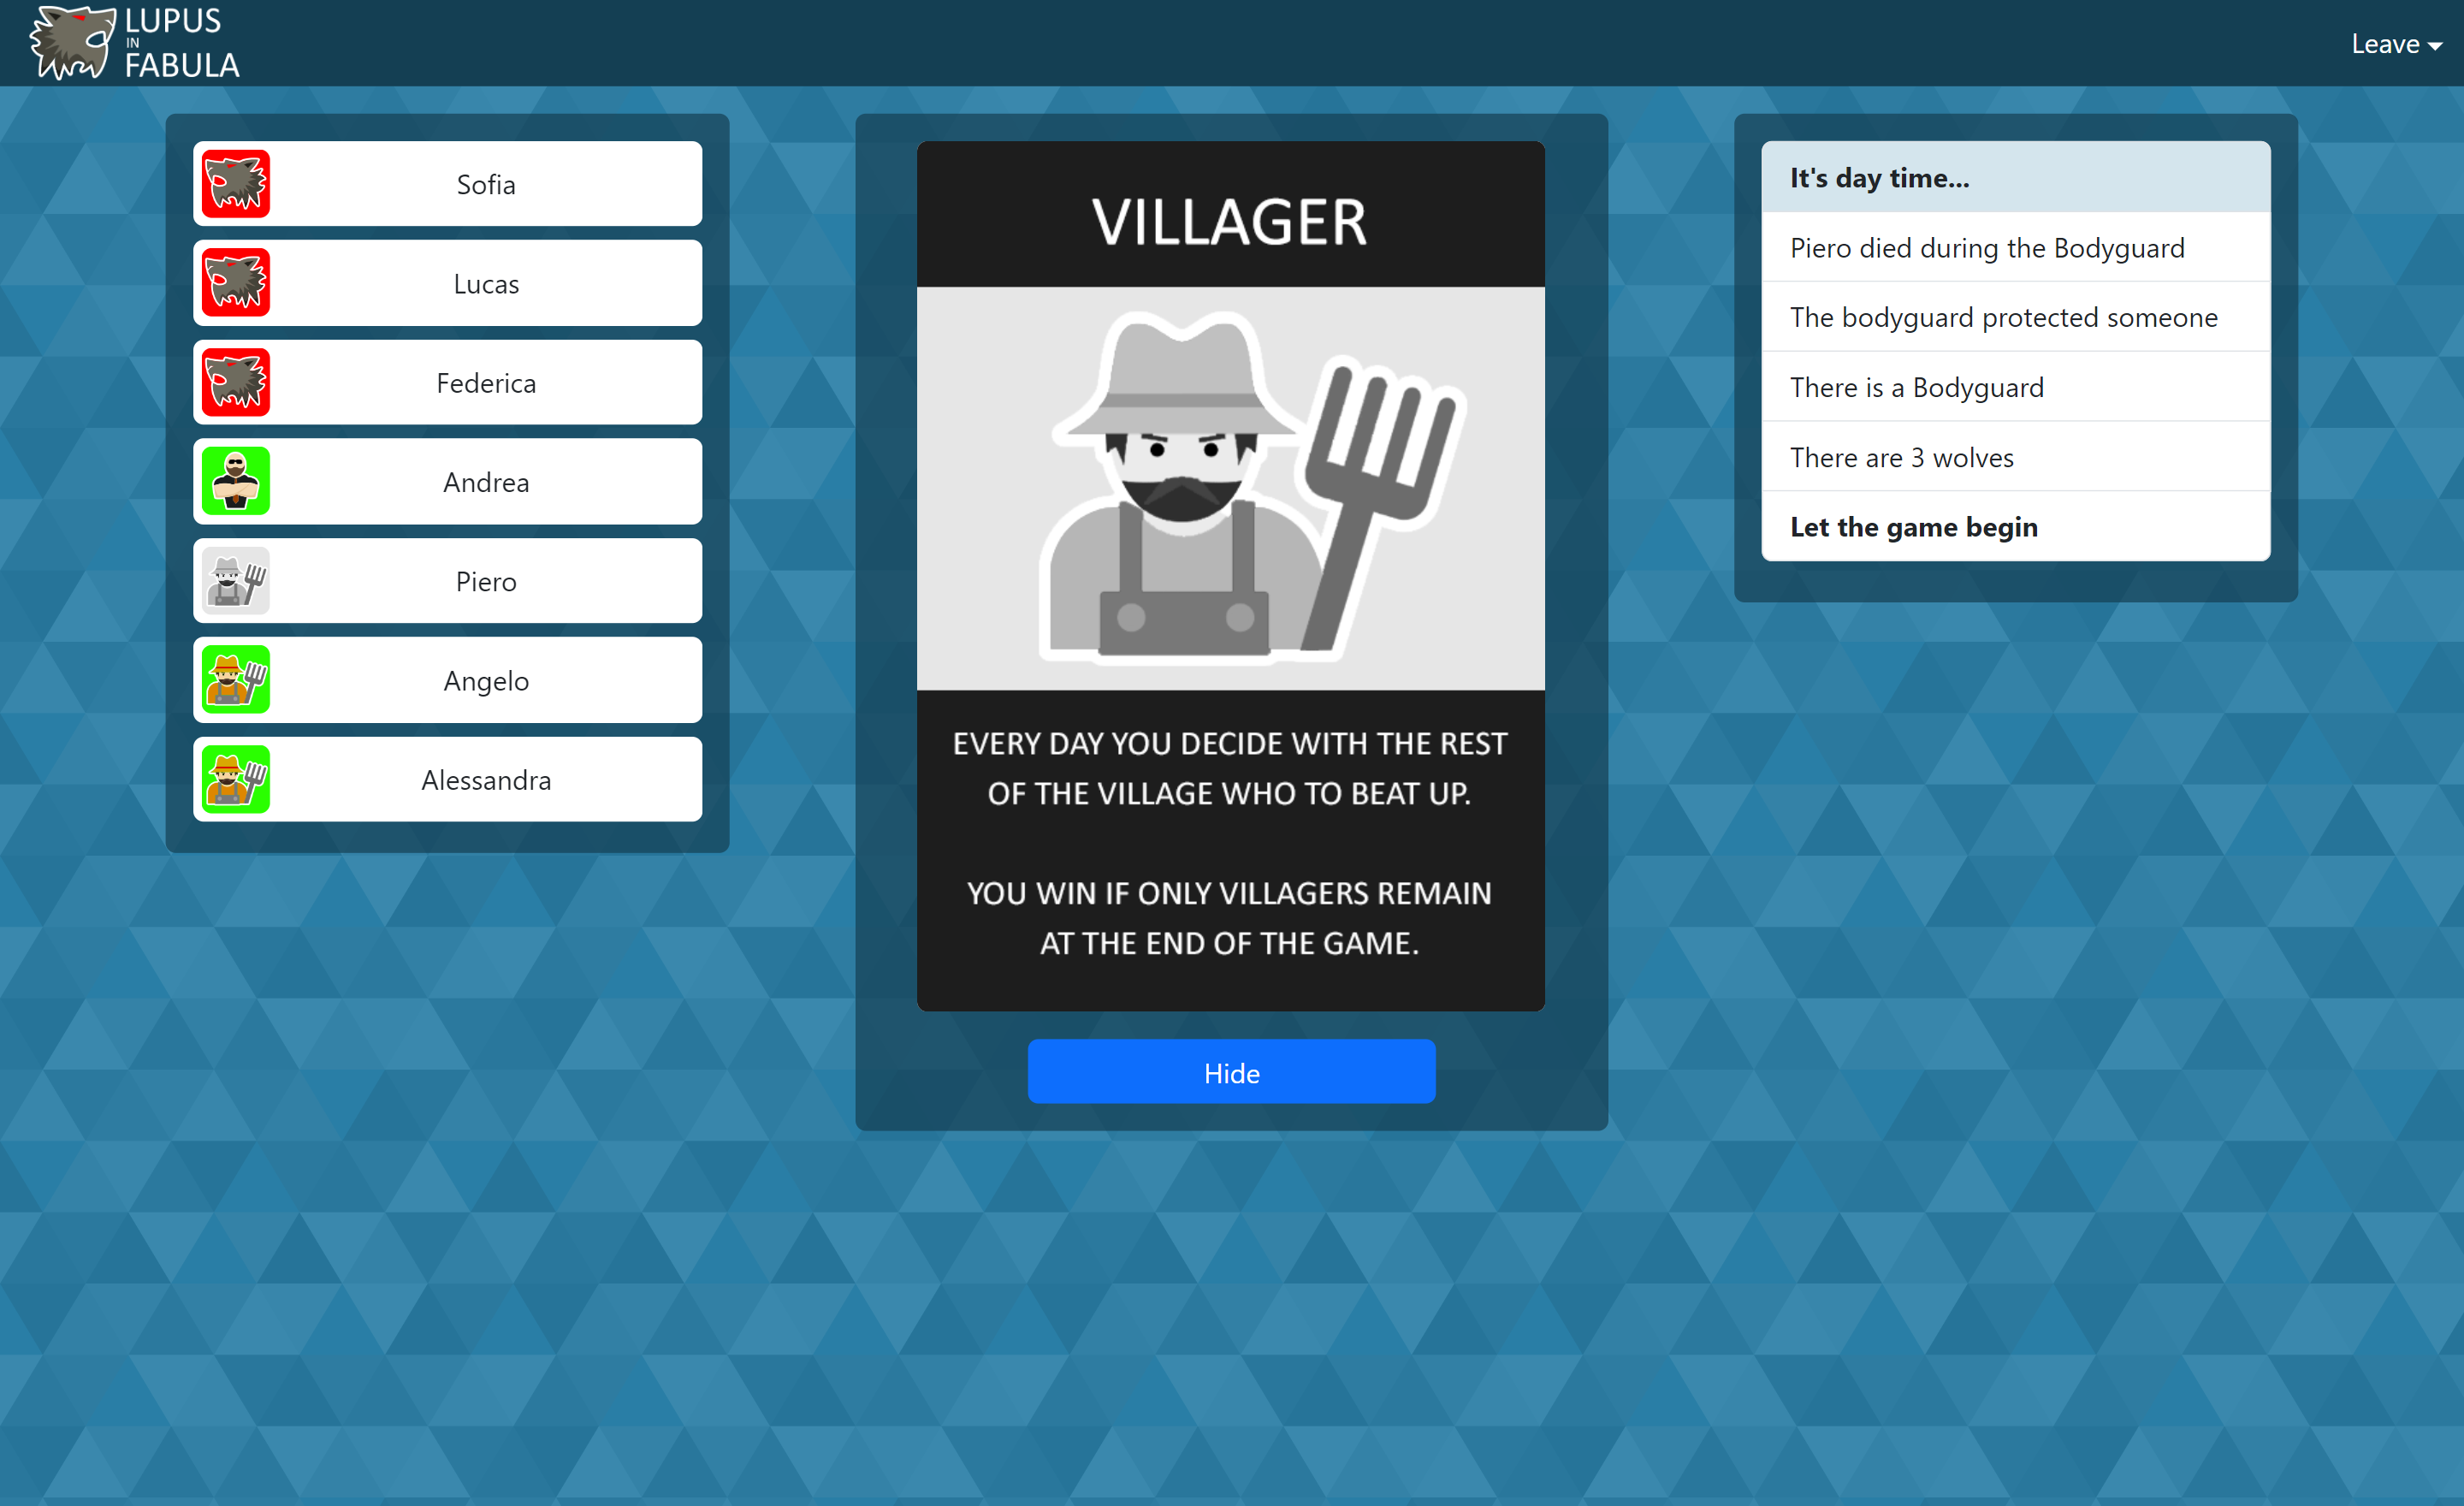
\includegraphics[width=\textwidth]{img/screen/desktop/dead_desktop.png}
\caption{Schermata del giocatore morto}
\label{fig:dead_desktop}
\end{figure}

\begin{figure}[H]
\centering
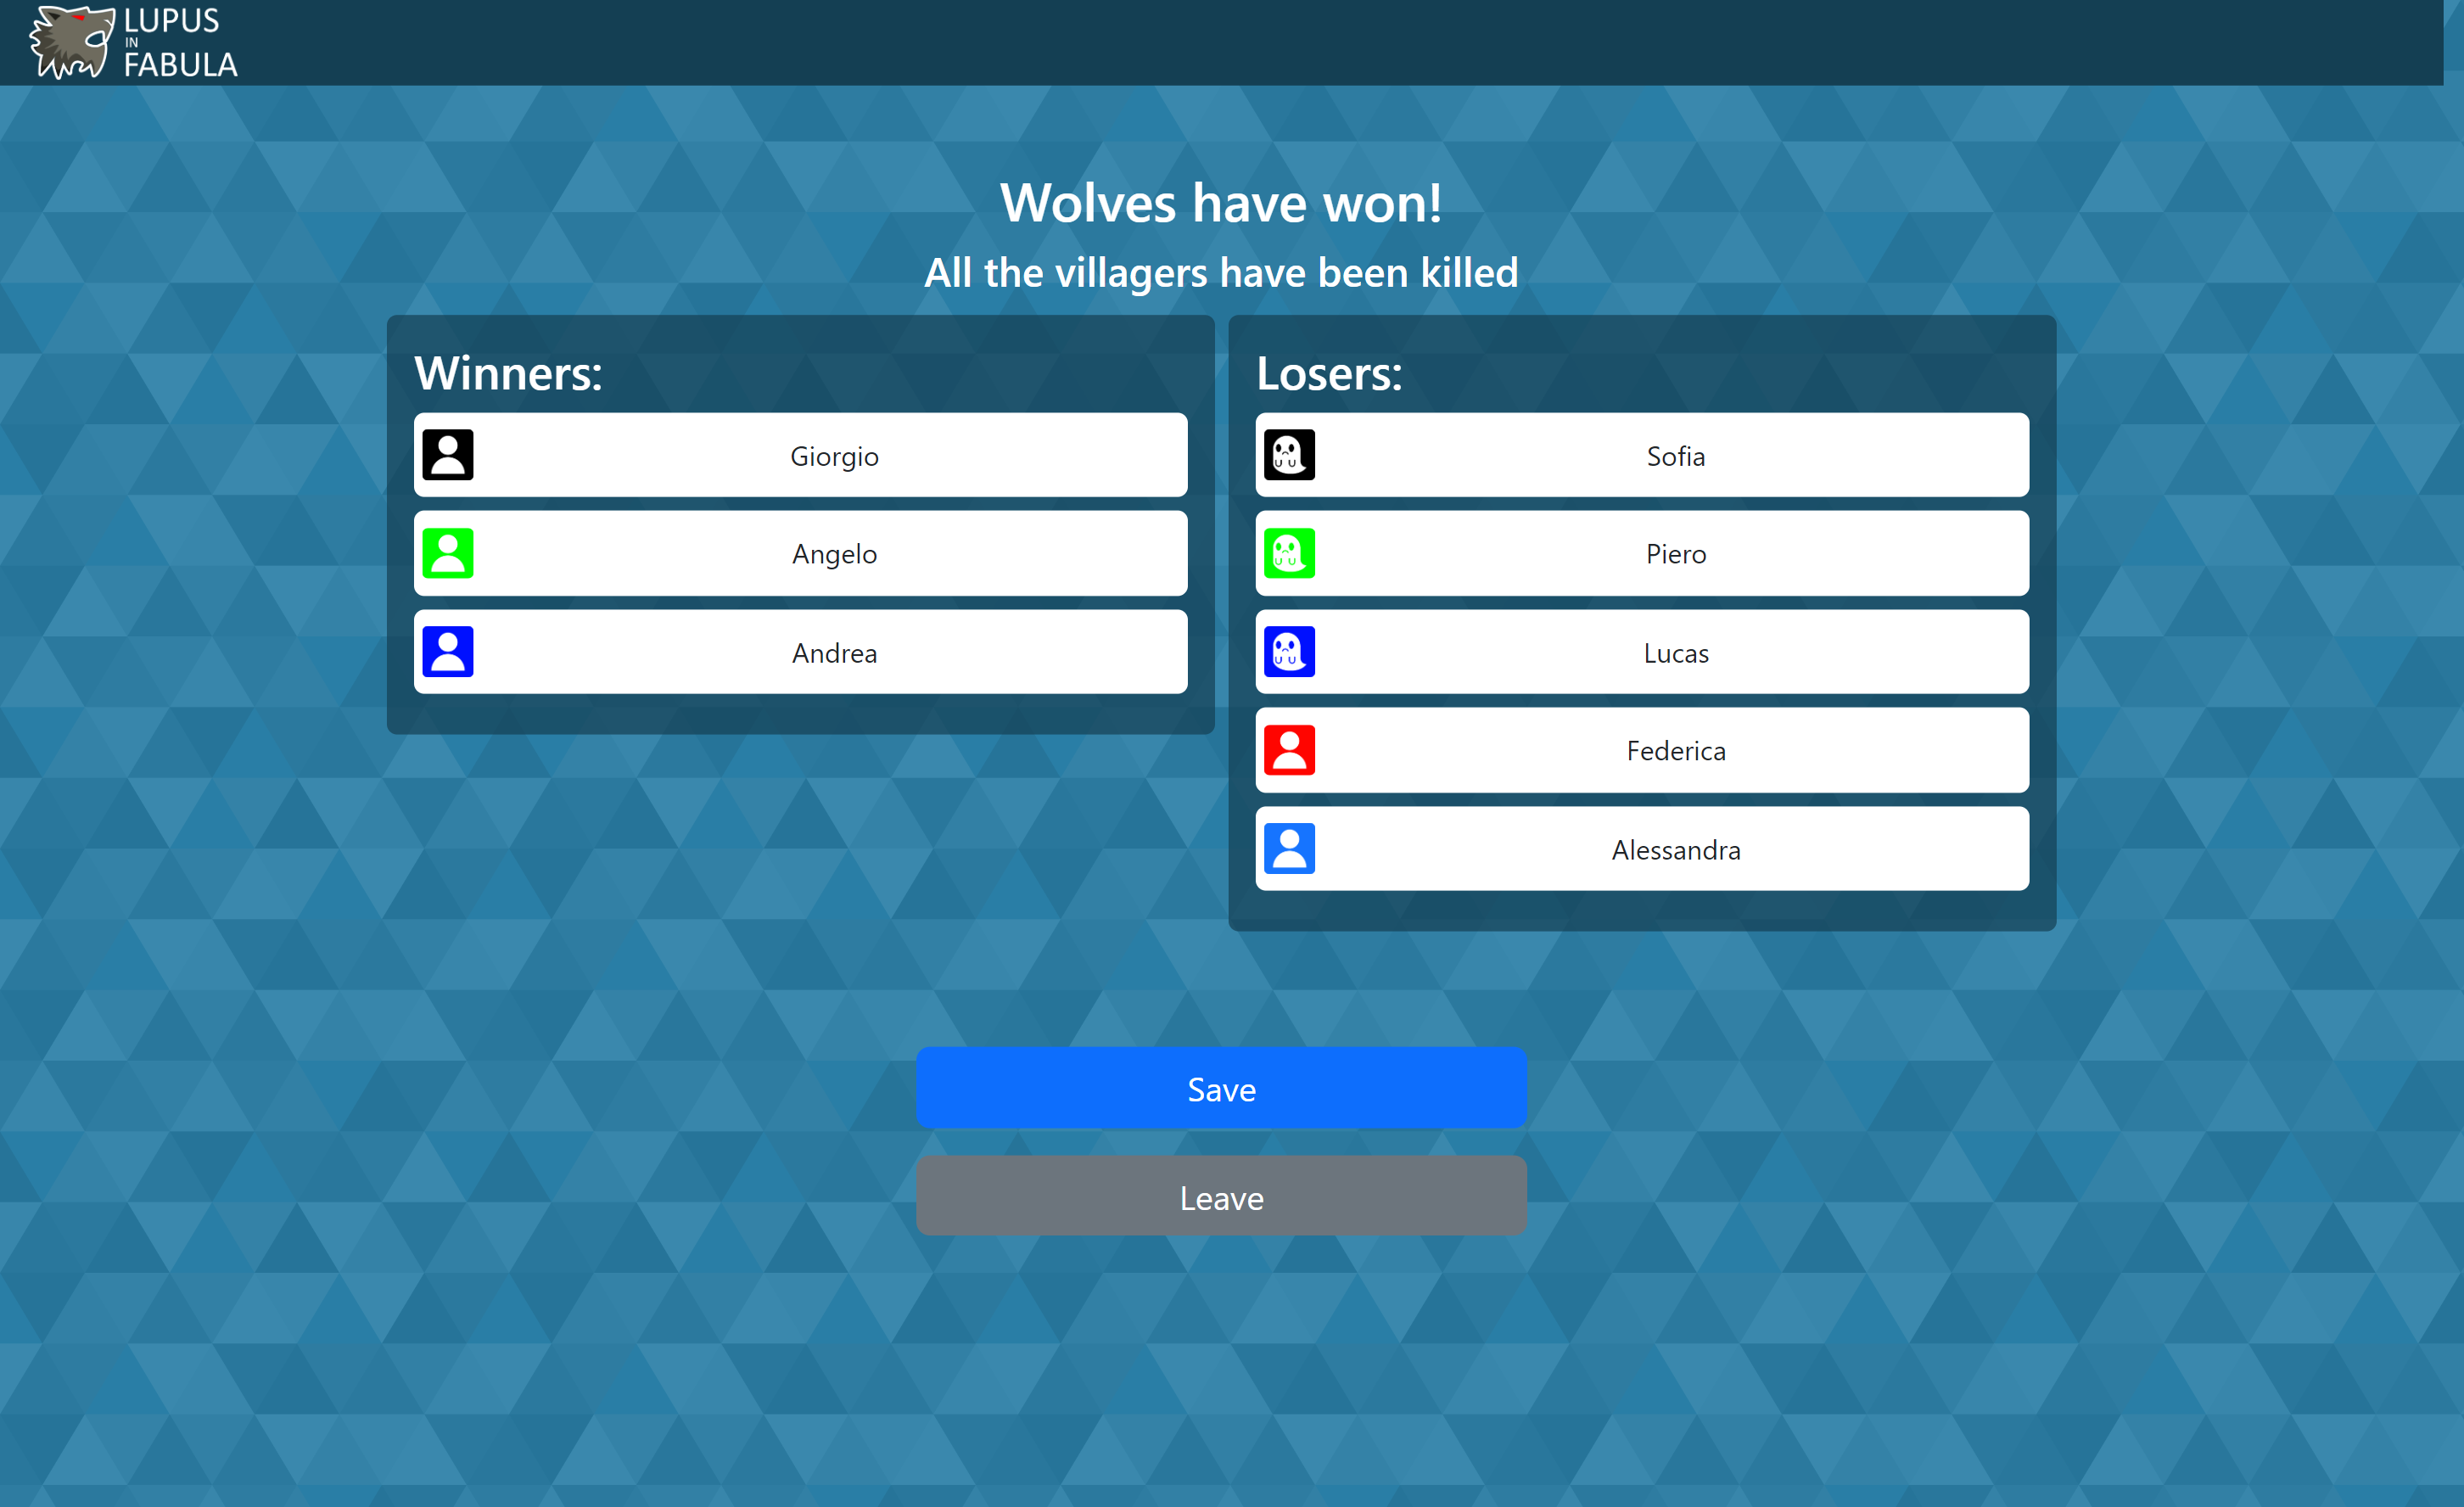
\includegraphics[width=\textwidth]{img/screen/desktop/won_desktop.png}
\caption{Schermata di fine partita}
\label{fig:won_desktop}
\end{figure}

\begin{figure}[H]
\centering
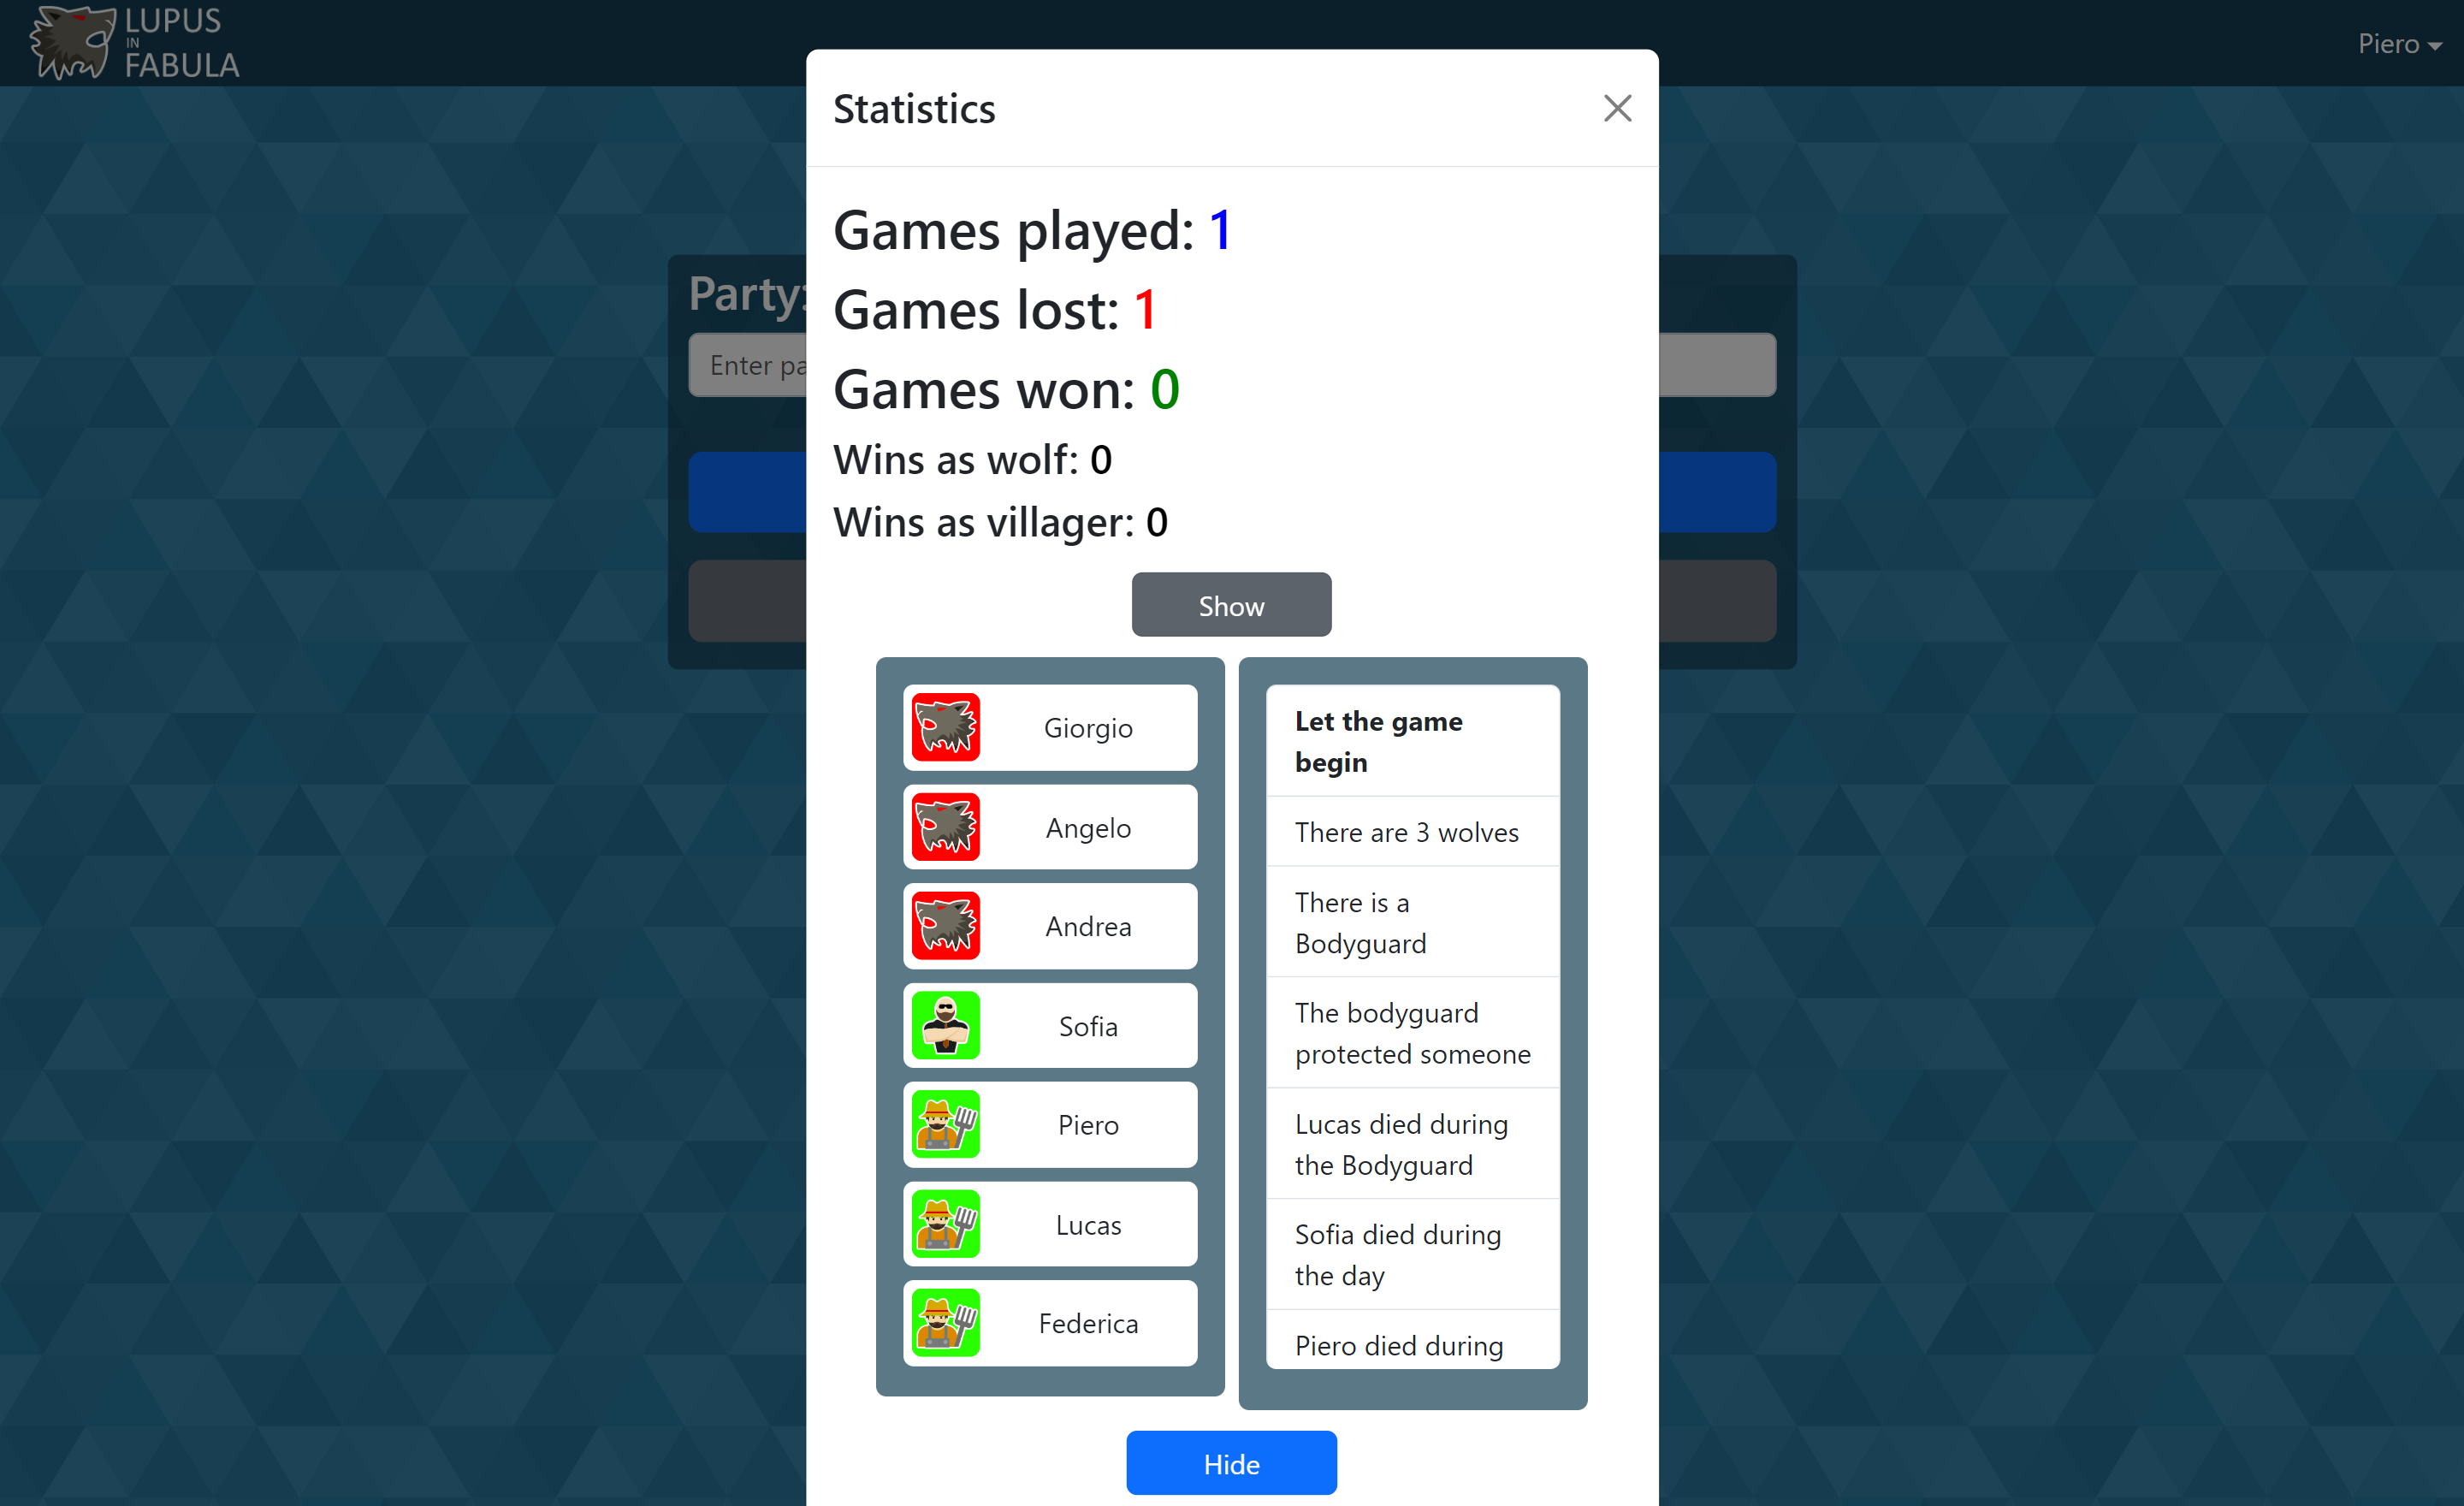
\includegraphics[width=\textwidth]{img/screen/desktop/stats_desktop.png}
\caption{Schermata delle statistiche del giocatore}
\label{fig:stats_desktop}
\end{figure}

\begin{figure}[H]
\centering
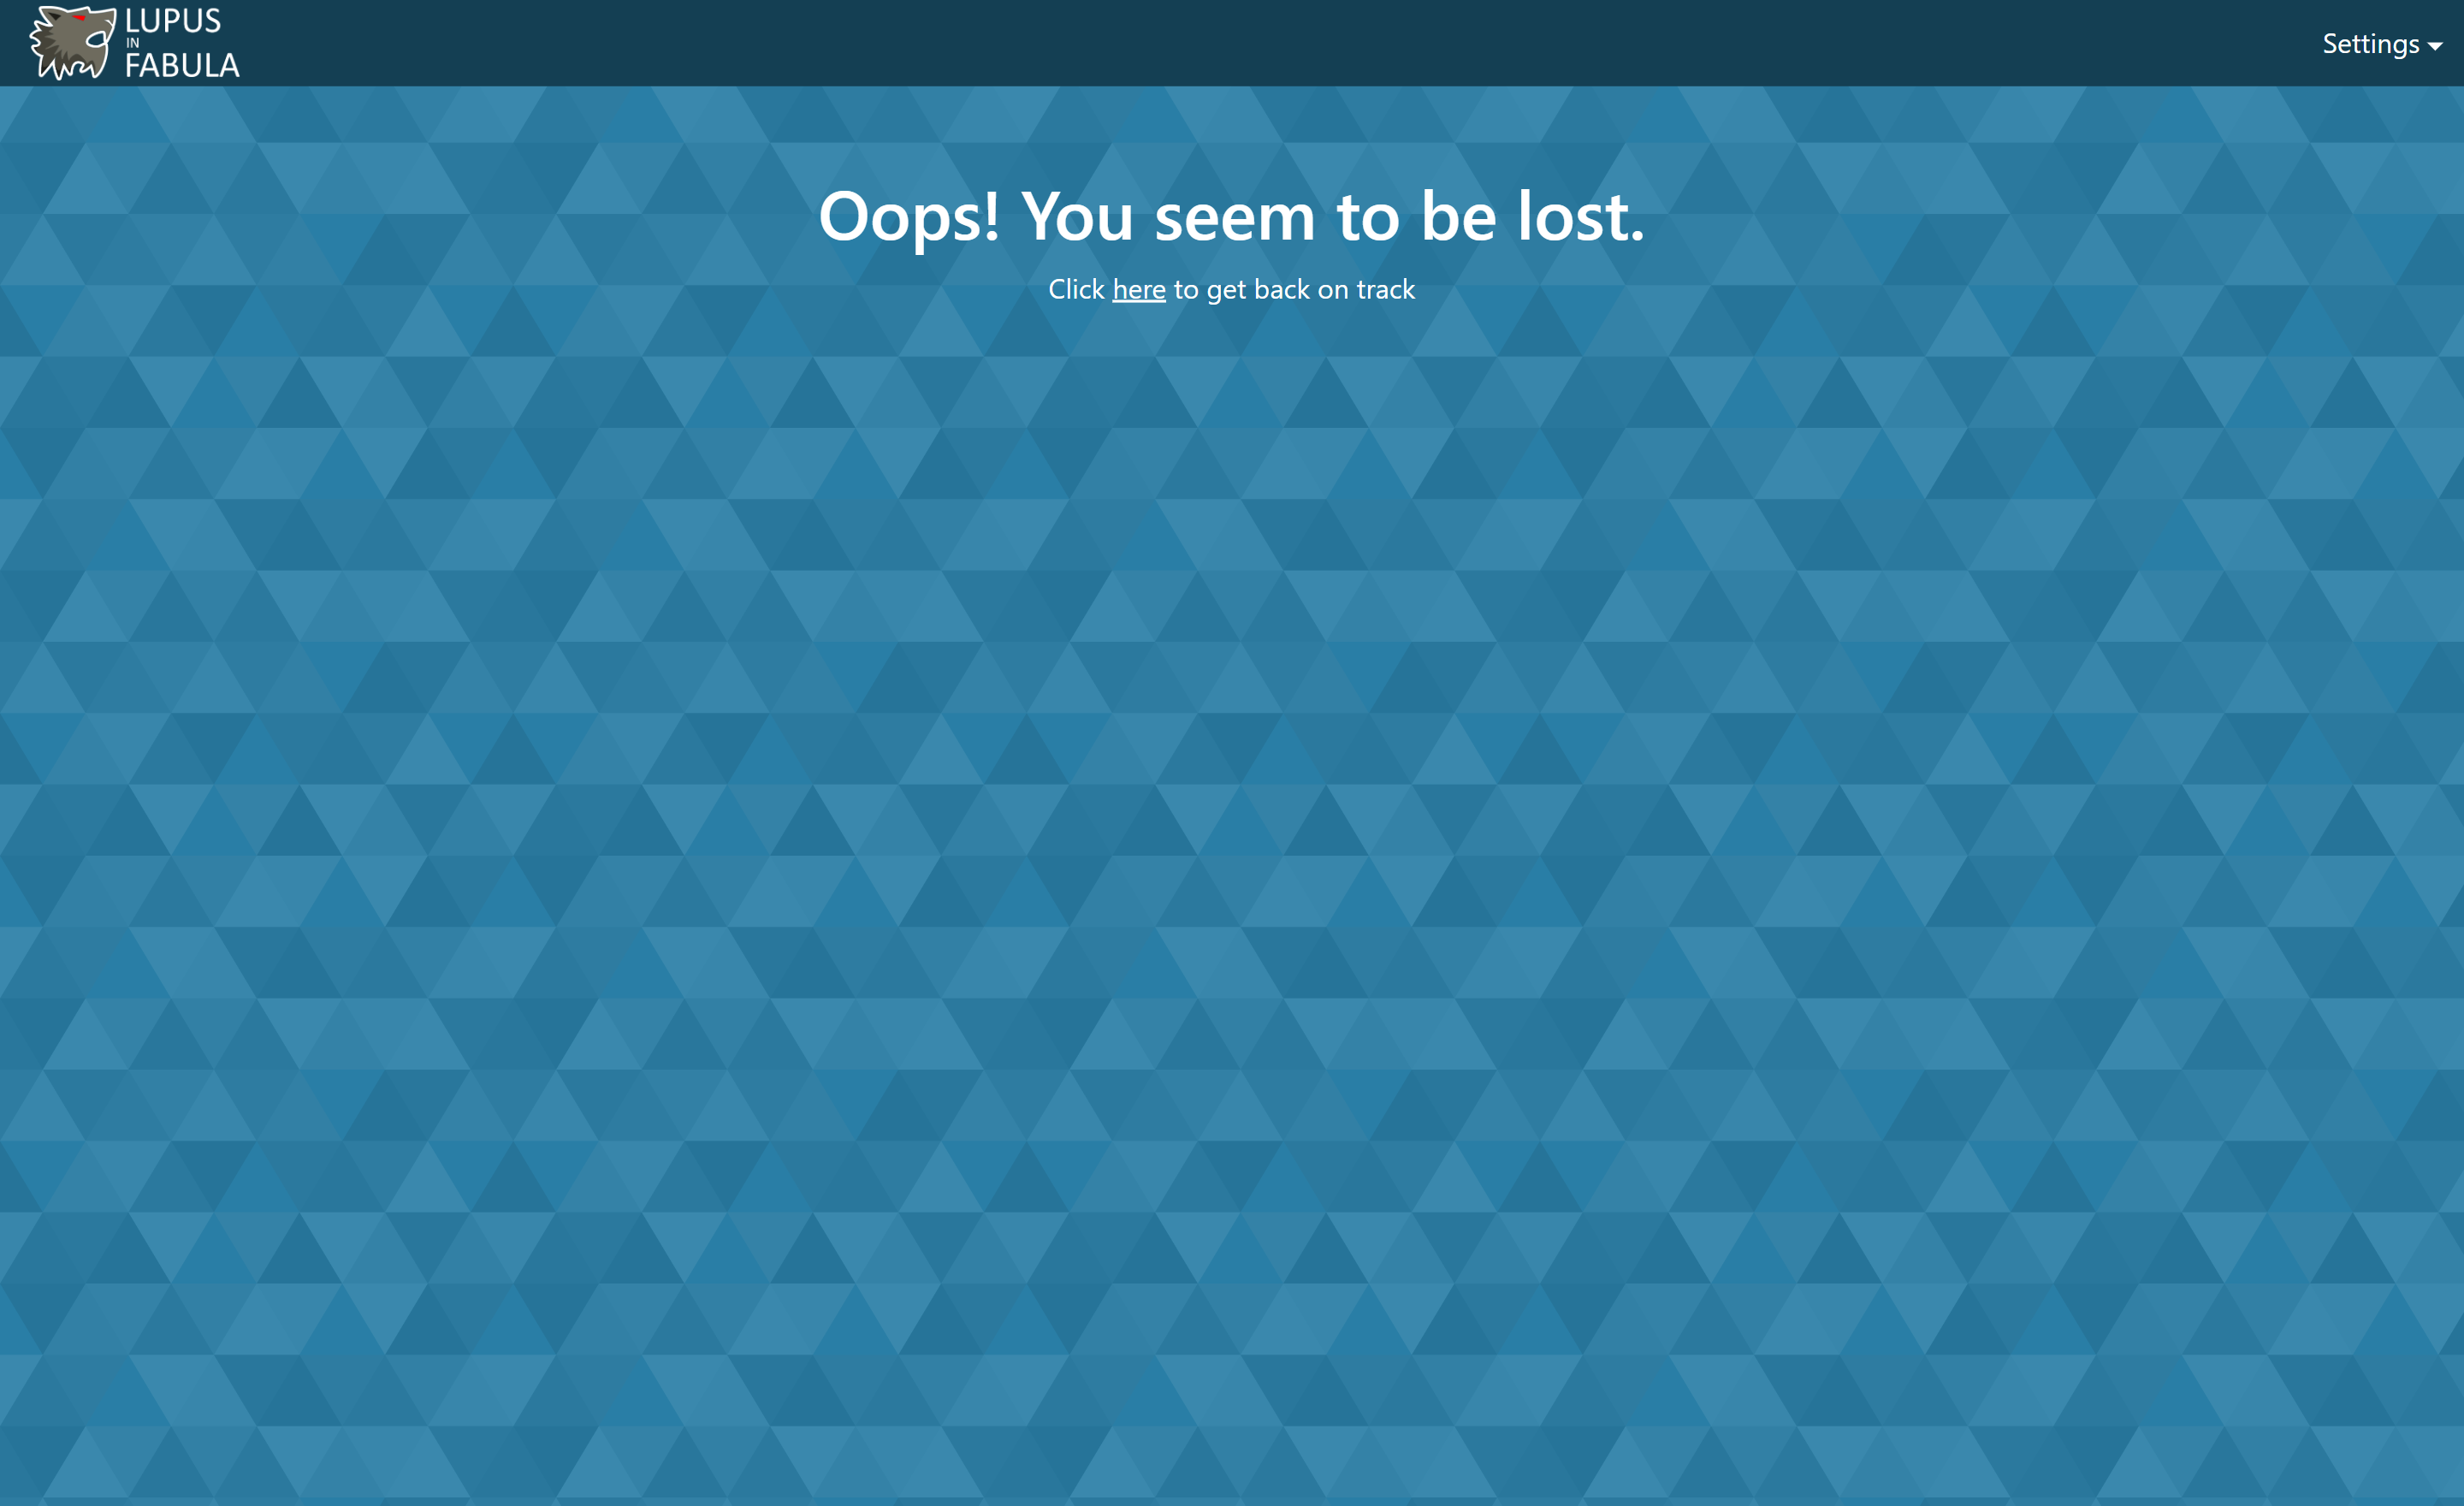
\includegraphics[width=\textwidth]{img/screen/desktop/404_desktop.png}
\caption{Schermata 404 indirizzo non trovato}
\label{fig:404_desktop}
\end{figure}

\chapter{Mobile screenshots}\label{appendix:mobile}


\begin{figure}[H]
    \centering
    \begin{minipage}{0.45\textwidth}
        \centering
        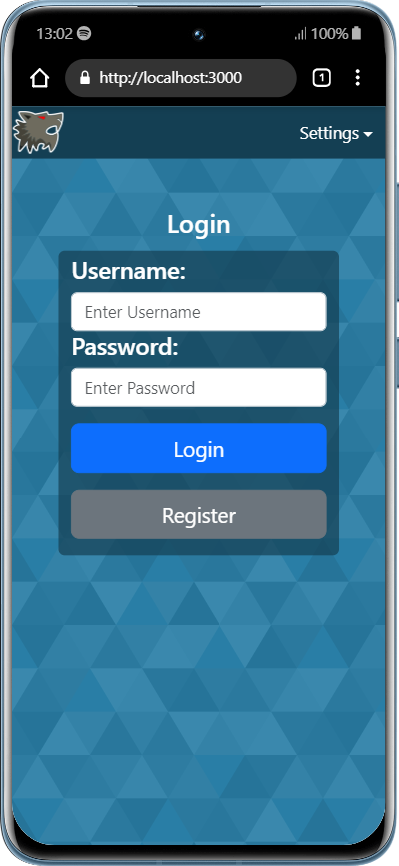
\includegraphics[width=0.9\textwidth]{img/screen/mobile/login_mobile.png}
        \caption{Schermata di autenticazione}
        \label{fig:login_mobile}
    \end{minipage}\hfill
    \begin{minipage}{0.45\textwidth}
        \centering
        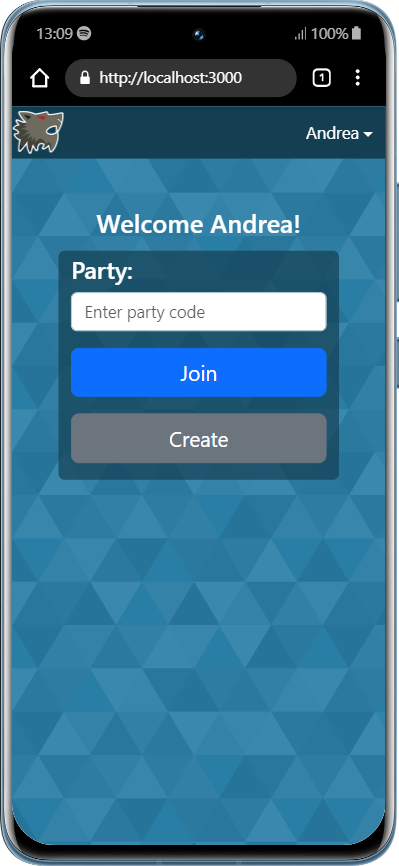
\includegraphics[width=0.9\textwidth]{img/screen/mobile/party_mobile.png}
        \caption{Schermata di selezione party}
        \label{fig:party_mobile}
    \end{minipage}
\end{figure}


\begin{figure}[H]
    \centering
    \begin{minipage}{0.45\textwidth}
        \centering
        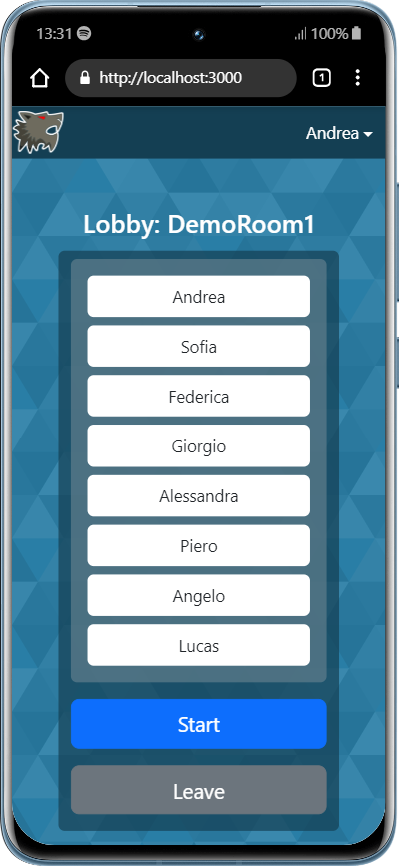
\includegraphics[width=0.9\textwidth]{img/screen/mobile/lobby_mobile.png}
        \caption{Schermata di lobby}
        \label{fig:lobby_mobile}
    \end{minipage}\hfill
    \begin{minipage}{0.45\textwidth}
        \centering
        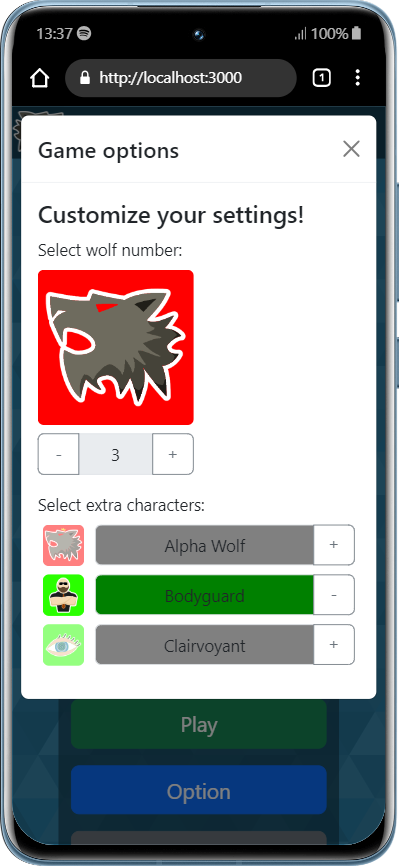
\includegraphics[width=0.9\textwidth]{img/screen/mobile/option_mobile.png}
        \caption{Schermata delle opzioni}
        \label{fig:option_mobile}
    \end{minipage}
\end{figure}

\begin{figure}[H]
    \centering
    \begin{minipage}{0.45\textwidth}
        \centering
        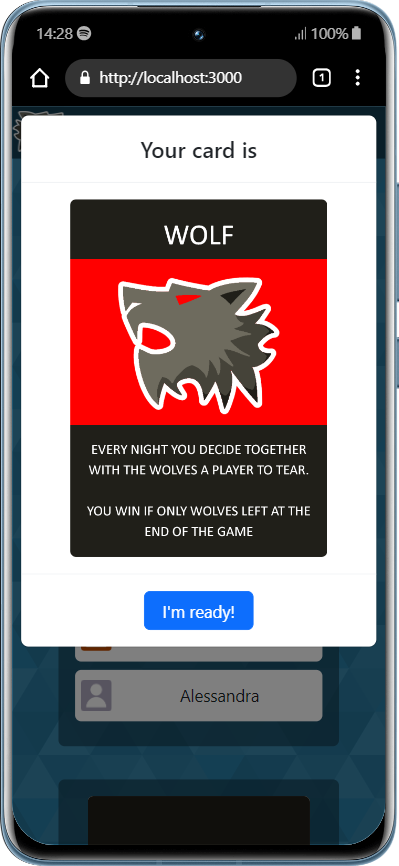
\includegraphics[width=0.9\textwidth]{img/screen/mobile/card_mobile.png}
        \caption{Schermata di inizio partita}
        \label{fig:card_mobile}
    \end{minipage}\hfill
    \begin{minipage}{0.45\textwidth}
        \centering
        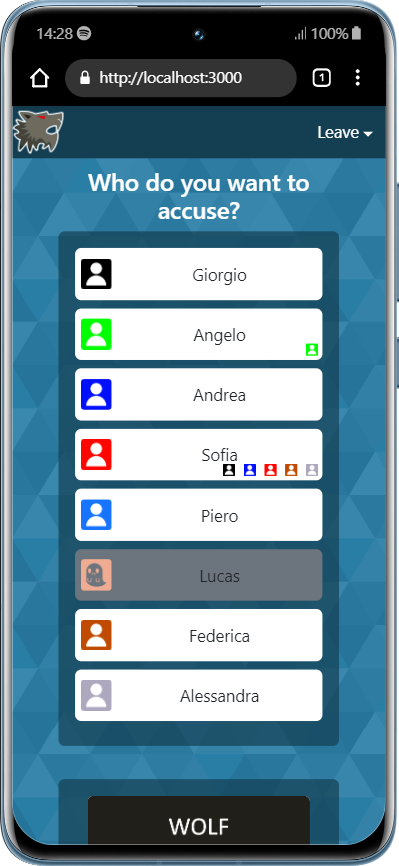
\includegraphics[width=0.9\textwidth]{img/screen/mobile/accusation_mobile.png}
        \caption{Schermata di turno di accusa}
        \label{fig:accusation_mobile}
    \end{minipage}
\end{figure}

\begin{figure}[H]
    \centering
    \begin{minipage}{0.45\textwidth}
        \centering
        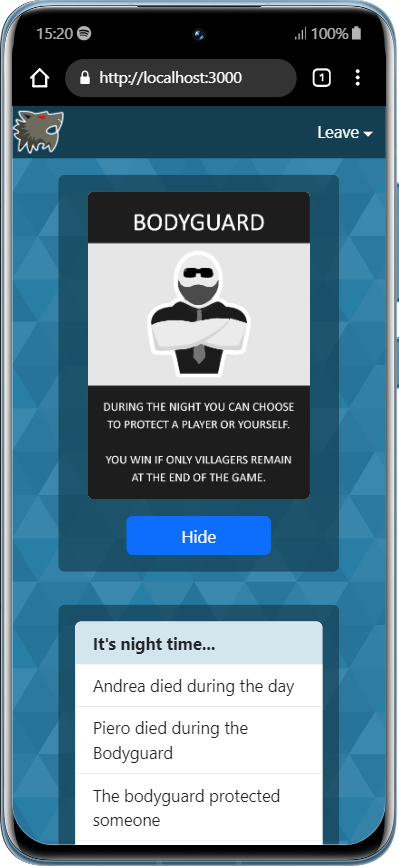
\includegraphics[width=0.9\textwidth]{img/screen/mobile/dead_mobile.png}
        \caption{Schermata del giocatore morto}
        \label{fig:dead_mobile}
    \end{minipage}\hfill
    \begin{minipage}{0.45\textwidth}
        \centering
        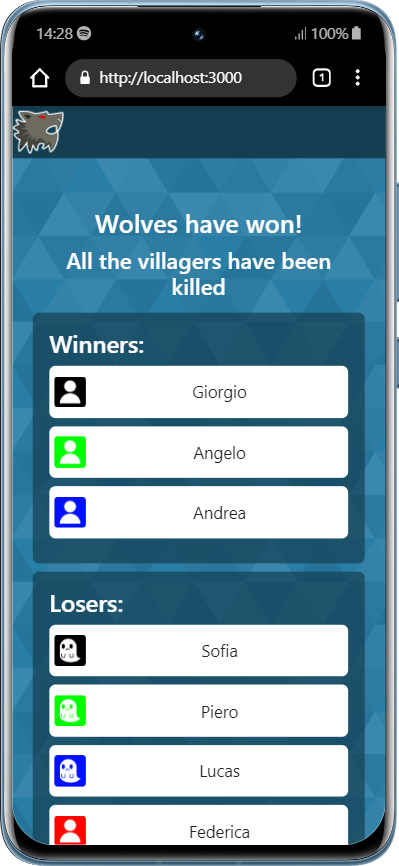
\includegraphics[width=0.9\textwidth]{img/screen/mobile/won_mobile.png}
        \caption{Schermata di fine partita}
        \label{fig:won_mobile}
    \end{minipage}
\end{figure}

\begin{figure}[H]
    \centering
    \begin{minipage}{0.45\textwidth}
        \centering
        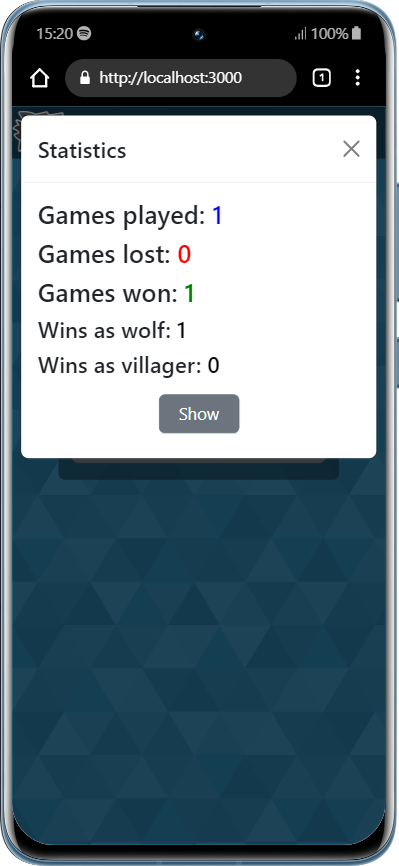
\includegraphics[width=0.9\textwidth]{img/screen/mobile/stats_mobile.png}
        \caption{Schermata delle statistiche del giocatore}
        \label{fig:stats_mobile}
    \end{minipage}\hfill
    \begin{minipage}{0.45\textwidth}
        \centering
        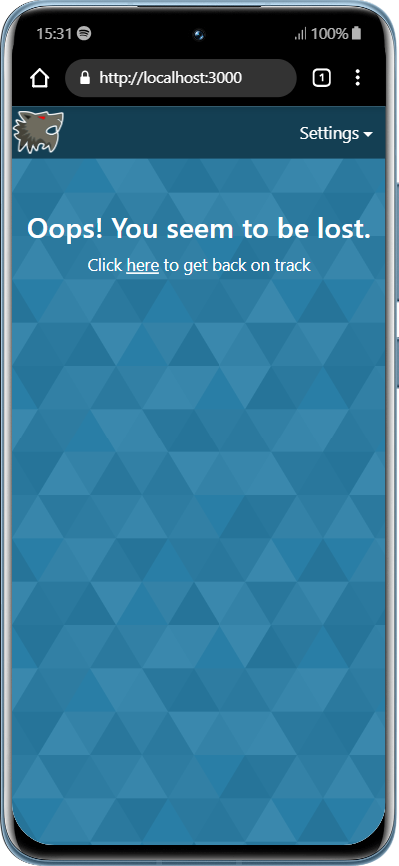
\includegraphics[width=0.9\textwidth]{img/screen/mobile/404_mobile.png}
        \caption{Schermata 404 indirizzo non trovato}
        \label{fig:404_mobile}
    \end{minipage}
\end{figure}

\begin{figure}[H]
    \centering
    \begin{minipage}{0.45\textwidth}
        \centering
        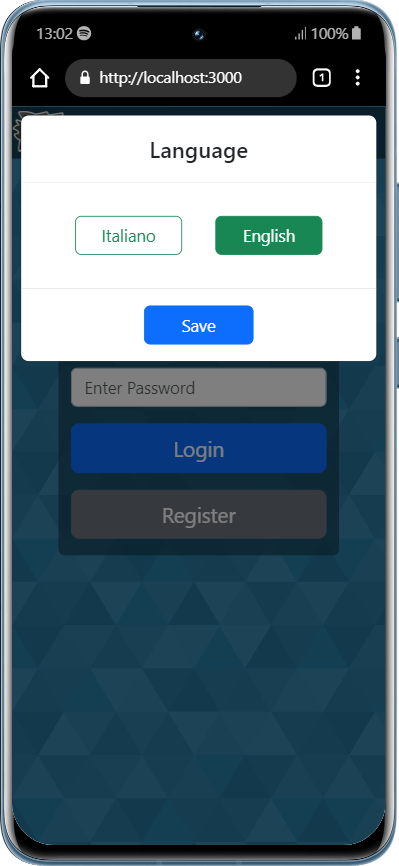
\includegraphics[width=0.9\textwidth]{img/screen/mobile/language_mobile.png}
        \caption{Schermata di settaggio lingua}
        \label{fig:language_mobile}
    \end{minipage}\hfill
\end{figure}


\nocite{*}
\bibliography{references}
\end{document}
